\documentclass[letterpaper,twocolumn,10pt]{article}
\usepackage{zhanggroup}

%-------------------------------------------------------------------------------
% Packages
% put your packages here
%-------------------------------------------------------------------------------

%-------------------------------------------------------------------------------
% Macros
% put your macros here
%-------------------------------------------------------------------------------

%-------------------------------------------------------------------------------
\begin{document}
%-------------------------------------------------------------------------------

\date{}

\title{Real Money, Fake Models: Deceptive Model Claims in Shadow APIs}

\author{
Yage Zhang \ \ \
Yukun Jiang \ \ \
Zeyuan Chen \ \ \
Michael Backes\ \ \
Xinyue Shen\ \ \
Yang Zhang\thanks{Corresponding author}
\\
\\
\textit{CISPA Helmholtz Center for Information Security} 
}
%\author{
%{Yang Zhang}\\
%CISPA Helmholtz Center\\ for Information Security
%%\and
%%{\rm Yang Zhang}\\
%%CISPA Helmholtz Center for Information Security
%} % end author

\maketitle

%-------------------------------------------------------------------------------
\begin{abstract}
Access to frontier large language models (LLMs), such as GPT-5 and Gemini-2.5, is often hindered by high pricing, payment barriers, and regional restrictions.
These limitations drive the proliferation of \textit{shadow APIs}, third-party services that claim to provide access to official model services without regional limitations via indirect access.
Despite their widespread use, it remains unclear whether shadow APIs deliver outputs consistent with those of the official APIs, raising concerns about the reliability of downstream applications and the validity of research findings that depend on them.
In this paper, we present the first systematic audit between official LLM APIs and corresponding shadow APIs.
We first identify 17 shadow APIs that have been utilized in 187 academic papers, with the most popular one reaching 5,966 citations and 58,639 GitHub stars by December 6, 2025.
Through multidimensional auditing of three representative shadow APIs across utility, safety, and model verification, we uncover both indirect and direct evidence of deception practices in shadow APIs.
Specifically, we reveal performance divergence reaching up to $47.21\%$, significant unpredictability in safety behaviors, and identity verification failures in $45.83\%$ of fingerprint tests.
These deceptive practices critically undermine the reproducibility and validity of scientific research, harm the interests of shadow API users, and damage the reputation of official model providers.
\end{abstract}
%-------------------------------------------------------------------------------

%-------------------------------------------------------------------------------
\section{Introduction}
%-------------------------------------------------------------------------------

Frontier large language models (LLMs) have transformed numerous domains, becoming essential infrastructure for scientific research and daily applications~\cite{ECDGGGHKLLLMZM25,ZZLTWHMZZDDYCCJRLTLLNW23,BCEGHKLLLLNPRZ23}. 
By integrating advanced reasoning and domain knowledge, these models demonstrate enhanced effectiveness in complex tasks~\cite{WWSBIXCLZ22,O232,SATMWCSTCPPSGKSCMAWCMCGTLRBSKN23}.
Given that many frontier LLMs are proprietary or require substantial computational resources, local deployment is often infeasible. 
In recent years, access to these models has been mediated through commercial APIs provided by companies like OpenAI and Google~\cite{KS25,XWGZJ25,LBLTSYZNWKNYYZCMRAHZDLRRYWSOZYSKGCKHHCXSGHIZCWLMZK22}.
However, official APIs often impose high pricing, payment barriers, and strict geographical restrictions~\cite{CZZ23}.
For instance, the official OpenAI API cannot be accessed directly from several regions, such as China, Russia, and Iran~\cite{O252,B24}.
As a result, a vast third-party provider market has emerged, offering compatible endpoints at a lower cost and without regional limitations.
We refer to these services as \textit{shadow APIs} (illustrated in \autoref{fig:intro}), platforms that claim to generate the same output as official LLMs via indirect access.
% The emergence of Shadow APIs has significantly lowered the barrier to entry for LLM usage.
By December 6, 2025, the most popular shadow APIs have accumulated 58,639 GitHub stars and have been utilized in 187 academic papers with 5,966 cumulative citations. 
Most of these papers have accepted by top venues, such as ACL, CVPR, and ICLR (see details in \autoref{section:academia}).

\begin{figure}[t!]
    \centering
    \includegraphics[width=\linewidth]{Figures/intro.png}
    \caption{
        Comic for the production, transaction, use, and audit of shadow APIs. This illustration is partially generated by Nano Banana Pro~\cite{nanobananapro2025google} and manually refined.
    }
    \label{fig:intro}
\end{figure}

Recent studies have highlighted the unreliability of API access for open-source models~\cite{CSZS25,GLGC2024,SLZJZH24}, raising serious concerns about whether shadow APIs can faithfully replace official ones.
Users may treat shadow APIs as interchangeable substitutes for official APIs, considering the access problem mainly from a utility perspective, without conducting further verification.
However, from a supply chain perspective, shadow APIs function as black-box agencies where requests are routed, processed, and potentially manipulated across multiple unauthorized nodes. 
By exploiting official branding to serve unstable or misrepresented models at low prices, shadow APIs not only divert revenue from legitimate providers but also potentially damage the reputation of official models due to degraded user experience and illicit access from restricted regions.

In this paper, we address the fundamental opacity of the shadow API market by answering three research questions:

\begin{enumerate}[label=\textbf{RQ\arabic*:}, leftmargin=*, labelsep=0.5em, itemsep=0.5em]
    \item What shadow APIs currently exist, and to what extent are they used?
    \item Do shadow APIs perform consistently with official ones for any given request?
    \item What evidence can model verification methods provide?
\end{enumerate}

To address \textbf{RQ1}, we identify 17 shadow APIs and survey 187 academic papers to quantify the prevalence of these services (\autoref{section:academia}).
For \textbf{RQ2}, we conduct a multi-dimensional benchmarking across both utility and safety perspectives (\autoref{section:utility}).
Alarmingly, our experiments reveal significant performance inconsistencies between shadow APIs and official APIs.
On high-risk medical benchmarks like MedQA, the accuracy of the Gemini-2.5-flash model drops precipitously, from $83.82\%$ with the official API to approximately $37.00\%$ across all examined shadow APIs.
Besides, shadow APIs demonstrate unpredictable safety behavior compared to official APIs, with harmfulness scores either underestimated by about $0.23$ or amplified to nearly double.
Finally, for \textbf{RQ3}, we utilize model fingerprinting and output metadata analysis to audit these shadow APIs. 
We provide concrete evidence of model substitution, confirmed by significant anomalies.
Specifically, across 24 evaluated endpoints, $45.83\%$ fail fingerprint verification, and an additional $12.50\%$ exhibit substantial cosine distance deviations from the official models (\autoref{section:fingerprinting}).

Our contributions are summarized as follows.
\begin{itemize}[leftmargin=*]
    \item We identify 17 widely used shadow APIs and present the first systematic audit on them compared with the official baselines.
    \item We demonstrate frequent failures and unreliability of shadow APIs in utility and safety evaluation, exposing their deceptive model claims.
    \item Verification based on model fingerprint and meta information provides supportive evidence of the differences between shadow and official APIs.
    \item Furthermore, we provide suggestions to enforce provenance awareness and reduce reproducibility risks when using LLM APIs.
\end{itemize}

\mypara{Disclosure}
We are committed to responsibly reporting our findings to official model providers as well as the authors of papers that use shadow APIs. 
We have received partial acknowledgment from them.

%-------------------------------------------------------------------------------
\section{Preliminary}
%-------------------------------------------------------------------------------

%-------------------------------------------------------------------------------
\subsection{Background}
%-------------------------------------------------------------------------------

LLMs have rapidly become the backbone of modern natural language processing (NLP), machine learning (ML), as well as even computer vision (CV) research, and the base for building personal agents such as OpenClaw~\cite{JZSBZ26}.
A recent analysis of 16{,}193 papers shows that by 2024, over $60\%$ of NLP papers, around $20\%$ of ML papers, and nearly $10\%$ of CV papers are related to LLMs~\cite{XZLCLLWL25}. 
The number of LLM papers has exploded from a few hundred in 2019 to more than 7{,}000 in 2024.
At the same time, access to frontier proprietary models is tightly controlled. 
Providers restrict API access to certain regions for legal and security reasons~\cite{G25}. 
For instance, Anthropic explicitly disallows sales in unsupported regions~\cite{A25}.
OpenAI likewise warns that accessing or reselling its API from unsupported countries may lead to account suspension~\cite{O24}.
These restrictions collide with the geographic barriers of artificial intelligence (AI) research, given the reality that major AI conferences such as AAAI and CVPR attract large numbers of submissions and accepted papers from regions with restricted access to frontier APIs (e.g., China)~\cite{A252,L24}.

In addition to geographic barriers, expensive bills put pressure on users.
Frontier LLM APIs are typically priced for enterprise customers, which can be prohibitive for individual researchers or students. 
Analysis of LLM API economics suggests that many current usage patterns are unsustainable for small actors without cross-subsidies~\cite{A253}.
This drives the rise of a commercial shadow market offering discounted access to frontier LLMs without geographical restrictions~\cite{Q252,K24}.

Moreover, official terms of service prohibit any form of API key resale or redistribution~\cite{O251}.
In addition, Chinese government regulations require AI services to operate in compliance with applicable laws and administrative requirements~\cite{CAC23}.
As a result, these sellers operate in violation of both the service contract and applicable regulatory requirements.
These trends suggest a growing disconnect between academic demand for frontier models and the constraints of official distribution channels, which drives the emergence of a substantial market of unofficial third-party services.

%-------------------------------------------------------------------------------
\subsection{Definition}
%-------------------------------------------------------------------------------

For clarity, we introduce the term \textit{shadow APIs} to describe third-party LLM API services characterized by
(i) \textbf{indirect access}, and
(ii) \textbf{access provision in restricted regions}.

%-------------------------------------------------------------------------------
\subsection{Related Work}
%-------------------------------------------------------------------------------

LLMs exhibit distinct linguistic patterns and features that function as fingerprints, enabling the identification of the LLM that generated a given piece of content~\cite{MSSA25, YCWPWC23, BZTYZY23}.
\cite{PKA25} introduces LLMmap, an active fingerprinting method that queries models with carefully crafted inputs to estimate the likelihood of the response under different reference models.

\cite{CSZS25} audits model substitution in open-source LLM APIs and evaluates Trusted Execution Environments (TEEs) as a hardware-level solution for verifiable model integrity.
In contrast, we focus on the shadow APIs, indirect services that operate as opaque black boxes. 
Relatedly, research on model extraction and imitation~\cite{KTPPI19} shows that smaller models can be trained to mimic the outputs of frontier models, making it increasingly difficult for users to distinguish between authentic and distilled versions based on surface-level interactions alone.
However, systematic audits of indirect API services operating in this unregulated shadow market remain largely absent.

%-------------------------------------------------------------------------------
\section{Landscape of Shadow APIs}
\label{section:academia}
%-------------------------------------------------------------------------------
For \textbf{RQ1}, we investigate the prevalence of shadow APIs by quantifying their widespread adoption across both the research and the open-source community.

%-------------------------------------------------------------------------------
\subsection{Shadow APIs Collection}
%-------------------------------------------------------------------------------
We start from screening the accepted papers from ICLR 2024 (2{,}260 total, 1{,}108 with code) and papers from ACL 2024 (1{,}923 total, 1{,}005 with code)~\cite{I24,A24}. 
To retrieve the associated code repositories, we systematically parsed the abstracts and footnotes of these papers to extract URLs matching standard repositories.
From this combined pool of 2,113 code-available papers, we identify 92 projects that use LLM APIs via their associated GitHub repositories.
Among these, 21 papers ($22.8\%$) use at least one shadow API endpoint, and we search GitHub for these URLs to find additional repositories that call the same endpoint URL, collecting the venue, institution, country, citation counts, and the GitHub stars of associated repositories, with all metrics updated as of December 6, 2025. 
We iterate this process by harvesting new shadow API endpoint URLs from these repositories, repeating until no new ones are discovered. 

%-------------------------------------------------------------------------------
\subsection{Prevalence and Impact of Shadow APIs}
%-------------------------------------------------------------------------------

\mypara{Usage}
We ultimately identify 17 shadow APIs whose endpoints appear in 187 research papers. Among these, 116 papers ($62.03\%$) have been accepted at peer-reviewed conferences\footnote{For *ACL conferences, our statistics also encompass papers published in Findings.} or journals, such as ACL, CVPR, and ICLR.
The most widely used shadow API has accumulated 5,966 citations, and the associated GitHub repositories have received a total of 58,639 stars, as shown in~\autoref{figure:publish_counts}.
These results indicate that shadow API usage is already widespread in research.
As shown in~\autoref{figure:author_regions}, most authors are affiliated with institutions in regions such as China, where access to certain proprietary models is restricted.
These works also attract a large number of citations and substantial engagement on GitHub, as illustrated in~\autoref{figure:github_cites}.

\begin{figure*}[!t]
\centering
\begin{subfigure}{0.32\linewidth}
    \centering
    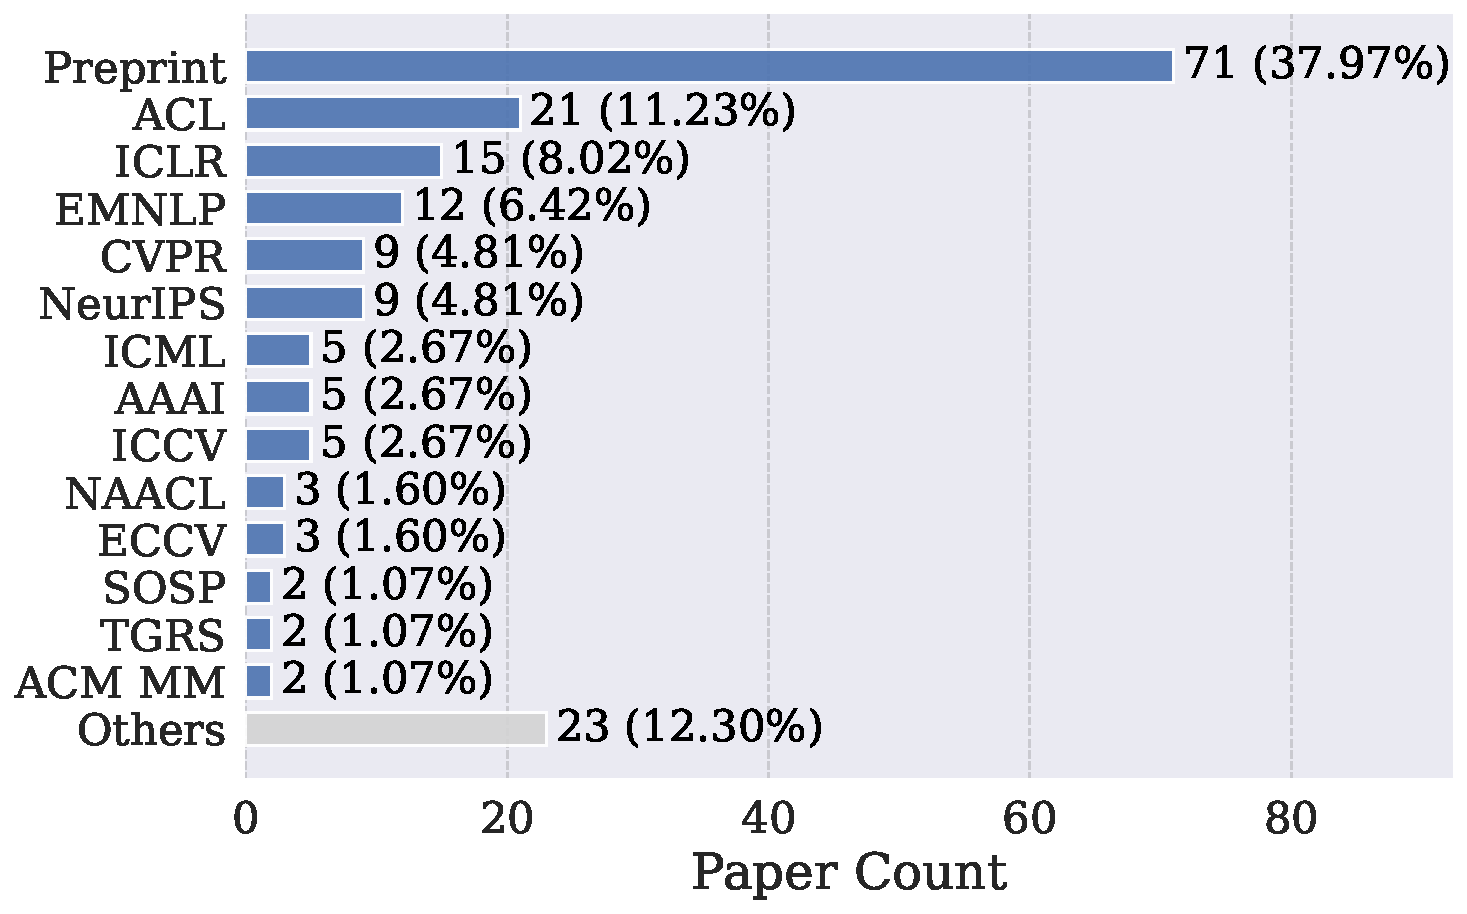
\includegraphics[width=\linewidth]{Figures/publish_distribution_top80.pdf}
    \caption{Paper counts by research venue.}
    \label{figure:publish_counts}
\end{subfigure}
\begin{subfigure}{0.30\linewidth}
    \centering
    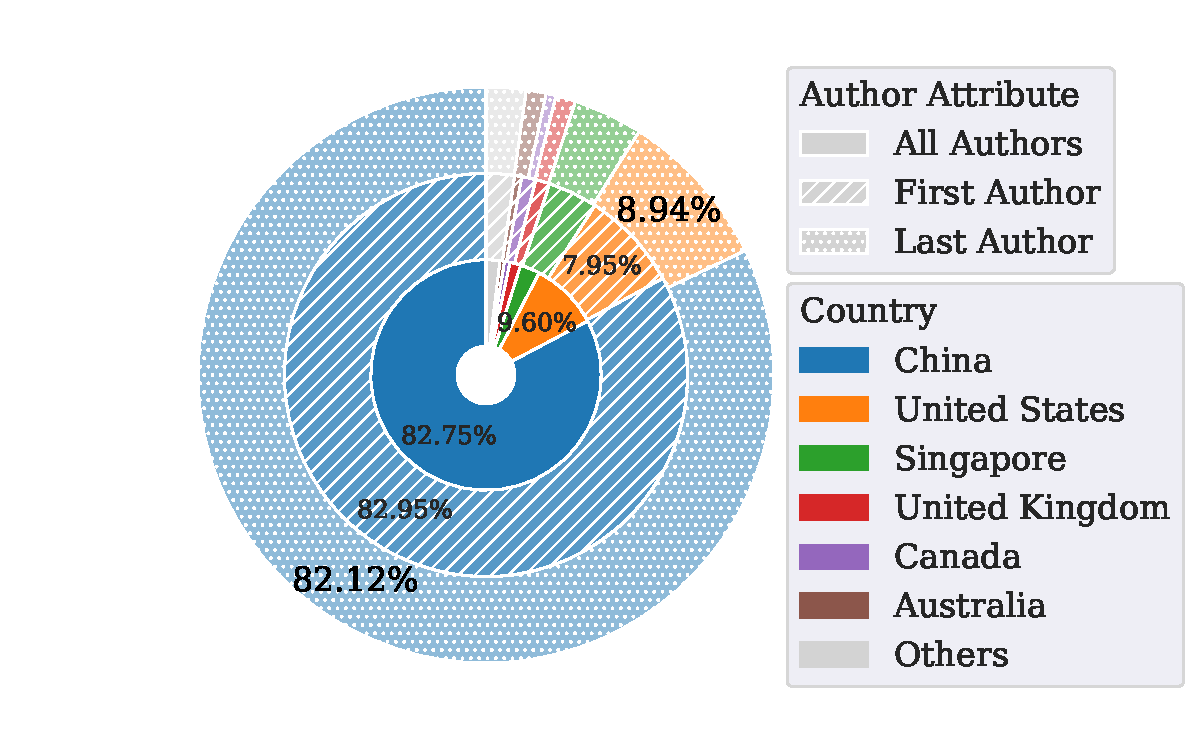
\includegraphics[width=\linewidth, trim={3.3cm 0 0 0}, clip]{Figures/nationality_pattern_donut.pdf}
    \caption{Geographic distribution of authors.}
    \label{figure:author_regions}
\end{subfigure}
\begin{subfigure}{0.34\linewidth}
    \centering
    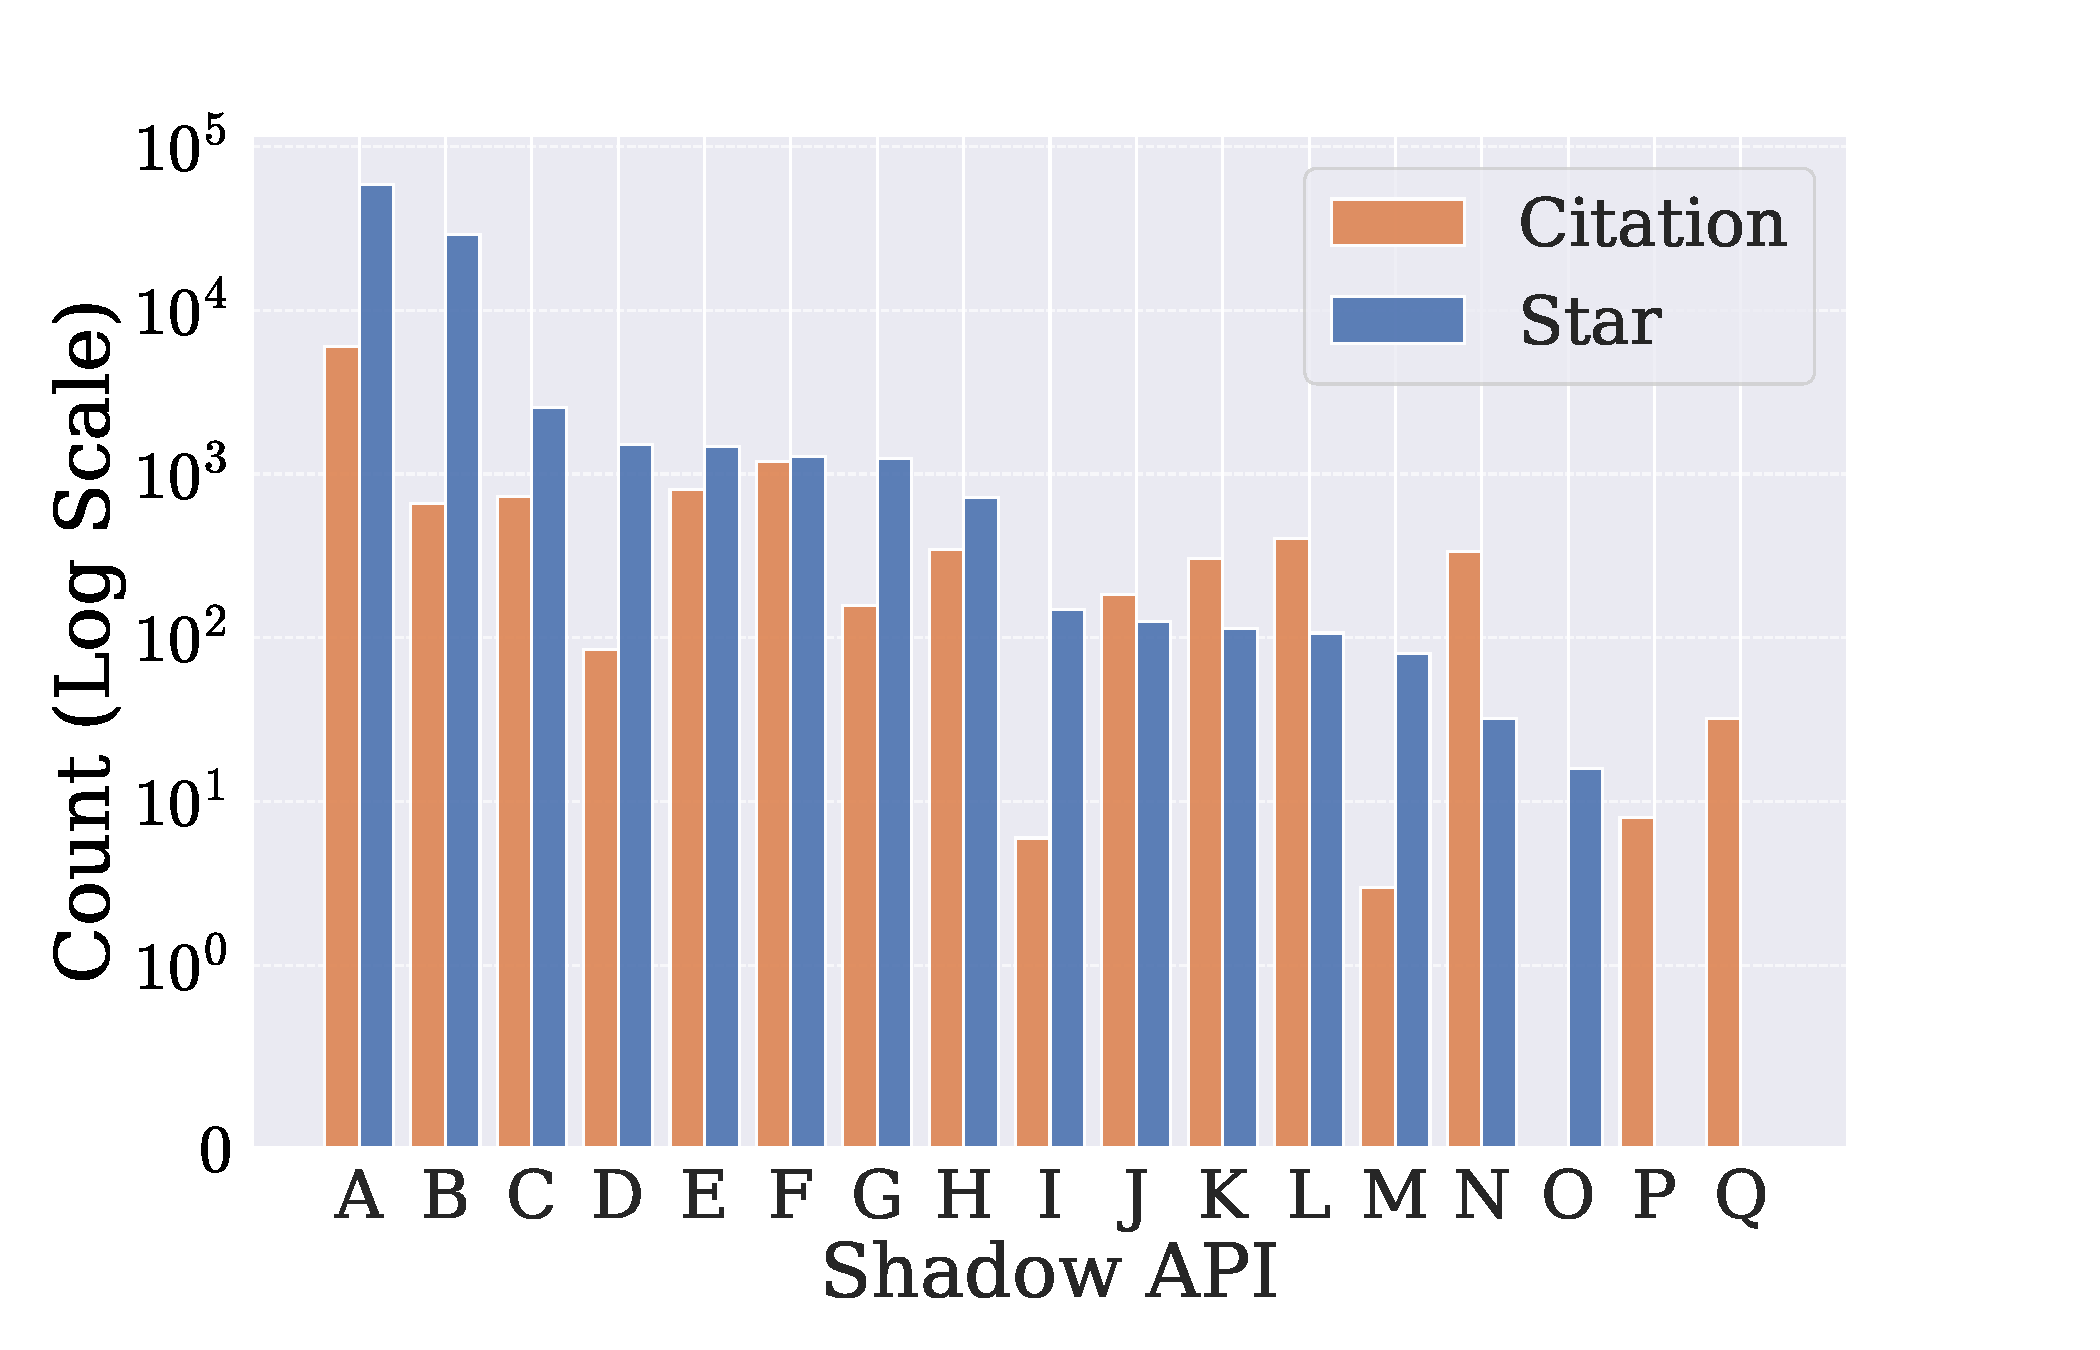
\includegraphics[width=\linewidth]{Figures/api_star_cite_symlog.pdf}
    \caption{Citations and GitHub stars.}
    \label{figure:github_cites}
\end{subfigure}
\caption{Landscape of the shadow APIs.}
\label{figure:overall_impact}
\end{figure*}

\mypara{Infrastructure} 
Among the 17 identified shadow API services, our analysis reveals that 11 are built upon open-source AI model aggregation and redistribution systems, primarily OneAPI~\cite{Q25} and its derivative, NewAPI~\cite{Q251}. 
OneAPI is an open-source tool designed for self-hosted deployment. 
It unifies interfaces from various commercial LLM providers into a standard OpenAI-compatible format. 
The infrastructure system supports key features such as API key management, secondary redistribution, request routing, and automatic retries, thereby increasing the potential for exploitation, resale, and abuse more than the official API.

\mypara{Compliance and Transparency}
The compliance and transparency of third-party API services are critical, as they determine whether users’ rights can receive legal protection, including whether the service operates as described and whether it can ensure continuous and stable availability.
To assess the compliance status of shadow APIs, we examine publicly available information on provider identity, corporate registration, and service-related disclosures.
Our analysis shows that 15 of the 17 identified services are operated by individuals without transparent identity information or verifiable provenance.  
Only one provider holds a valid corporate registration through an Internet Content Provider filing in China.  
As a result, the provider ecosystem exhibits high operational volatility, with two services having already ceased operations.  
In addition, all providers frequently change their upstream model sources, without providing users with detailed or transparent notifications regarding these changes.
This suggests that most shadow APIs operate without effective compliance verification or governance safeguards, thereby exposing users to elevated legal and operational risks.
Full compliance metadata for all 17 providers is provided in~\cref{appendix:anonymized_apis}.

\begin{tcolorbox}[colback=gray!25!white, size=title,breakable,boxsep=1mm,colframe=white,before={\vskip1mm}, after={\vskip0mm}]
\textbf{RQ1 Take-Aways:}
Shadow APIs are already widely popular in usage, yet they operate with minimal transparency and governance. 
Most providers lack verifiable identity, stable infrastructure, or disclosure of upstream models.
\end{tcolorbox}

%------------------
\section{Performance Evaluation}
\label{section:utility}
%------------------
To address \textbf{RQ2}, we evaluate the performance of shadow APIs via utility and safety benchmarks. 
We opt for this controlled approach over reproducing specific prior studies to mitigate the instability of shadow services and preserve the anonymity of affected researchers.

%------------------
\subsection{Experimental Setups}
%------------------

\mypara{Models}
To ensure a comprehensive evaluation across different providers and models, we select target models based on token usage statistics. 
We refer to the November 2025 usage ranking of LLMs on the OpenRouter public leaderboard, with the detailed chart provided in~\cref{appendix:ranking}.
From the ranking, we identify three primary model families (F-A, F-B, and F-C) covering both proprietary models and open-source model frontiers:
\begin{itemize}
    \item \textbf{F-A (OpenAI)}: GPT-4o-mini, GPT-5, and GPT-5-mini.
    \item \textbf{F-B (Google)}: Gemini-2.0-flash, Gemini-2.5-flash, and Gemini-2.5-pro.
    \item \textbf{F-C (DeepSeek)}: DeepSeek-Chat and DeepSeek-Reasoner.
\end{itemize}
For the science domain evaluation, we evaluate all the above eight LLMs.
For the sensitive domain and safety evaluations, we employ a filtered subset to focus on representative behaviors.
We select one distinct, widely deployed model from each family:
GPT-5-mini (representing F-A), Gemini-2.5-flash (representing F-B), and DeepSeek-Chat (representing F-C).

\mypara{Shadow API Selection}
To ensure the representativeness of our study, we select shadow APIs based on two popularity proxies, i.e., project citation counts and GitHub stars \cite{BHV16}.
We anonymize all providers and assign identifiers (shadow APIs A, B, etc.) based on a descending sort of their total citation counts, which are summarized in \autoref{figure:github_cites}.
The anonymized names for these shadow APIs are provided in~\autoref{table:api-capability-comparison}.
Specifically, we select shadow APIs A, E, and H based on three criteria: popular w.r.t. citations and GitHub stars, publicly accessible, and comprehensively covered for models in the three identified model families.
Anonymized brief profiles for these selected APIs are provided in~\cref{appendix:profiles}.
All official baselines are queried directly through the corresponding official APIs.

%-------------------------------------------------------------------------------
\mypara{Experimental Details}
%-------------------------------------------------------------------------------
To reduce variance, we average over three trials for all experiments and report accuracy with its standard deviation.
We perform utility and safety evaluations via API queries, which do not require local GPU acceleration. 
For the LLMmap method, we utilize an NVIDIA DGX A100 with GPU acceleration to train the model fingerprint database.
Detailed model configurations and API parameters are provided in \cref{appendix:model_configurations}.

%-------------------------------------------------------------------------------
\subsection{Utility Evaluation}
%-------------------------------------------------------------------------------

\mypara{Benchmarks and Methodology}
We assess model utility across scientific and sensitive domains~\cite{T25,D25,T251}.
For the science domain, we employ the AIME 2025 benchmark~\cite{A251}, which tests competition-level mathematics, and the GPQA (Diamond) benchmark~\cite{RHSPPDMB23}, targeting PhD-level scientific questions.
For the sensitive domain, we focus on high-risk fields, i.e., medical and legal fields.
In the medical field, following prior work~\cite{TSSCZXWZWSCG25}, we use the MedQA (USMLE) dataset~\cite{JPOWFS21}, covering diagnosis, treatment, and medical concepts.
In the legal field, we select LegalBench~\cite{GNHRCNCPWRZTHSFSDPHWNNNCTHMLRHKHRGGWGZIL23}, specifically the Scalr subset Rule-Application and Rule-Conclusion involving reasoning, consistent with~\cite{CTXWML25, HYGWKW25}.

\mypara{Implementation Details}
To ensure fair comparison, we adopt EvalScope prompt templates~\cite{C25} for the AIME 2025 and GPQA benchmarks, and for the MedQA (USMLE) benchmark, we use the Hulu-Med multiple-choice template~\cite {JWSHZPZYFZHCWTLXWXFZLXSWL25}, and the original task-specific prompts for LegalBench (Scalr)~\cite{GNHRCNCPWRZTHSFSDPHWNNNCTHMLRHKHRGGWGZIL23}.
We obtain all results using the model configurations detailed in \autoref{table:api-capability-comparison}.

\mypara{Science Domain Performance} 
The official API generally establishes the performance upper bound, as illustrated in~\autoref{fig:main_results}. 
Among the shadow APIs, shadow API E exhibits exceptional consistency, maintaining a minimal average divergence $2.64\%$ from the official. 
In some instances, such as with GPT-5-mini on GPQA, it even marginally outperforms the official API by $1.18\%$.
In contrast, official APIs exhibit minimal performance variance, whereas shadow APIs show substantially higher variability.
In particular, shadow APIs A and H display pronounced divergences from official APIs, with average accuracy gaps of $9.81\%$ and $6.46\%$, respectively.
Although these shadow APIs perform comparably on non-reasoning tasks, their performance degrades markedly on reasoning-oriented models.
Notably, on the AIME 2025 benchmark, shadow API A suffers severe accuracy drops, with deficits $40.00\%$ for Gemini-2.5-pro and $38.89\%$ for DeepSeek-Reasoner.
These results indicate that advanced reasoning capabilities are significantly compromised in shadow APIs A and H, resulting in substantial deviations from their claimed parity with official API performance.

\begin{figure}[!t]
\centering
\begin{subfigure}{\linewidth}
    \centering
    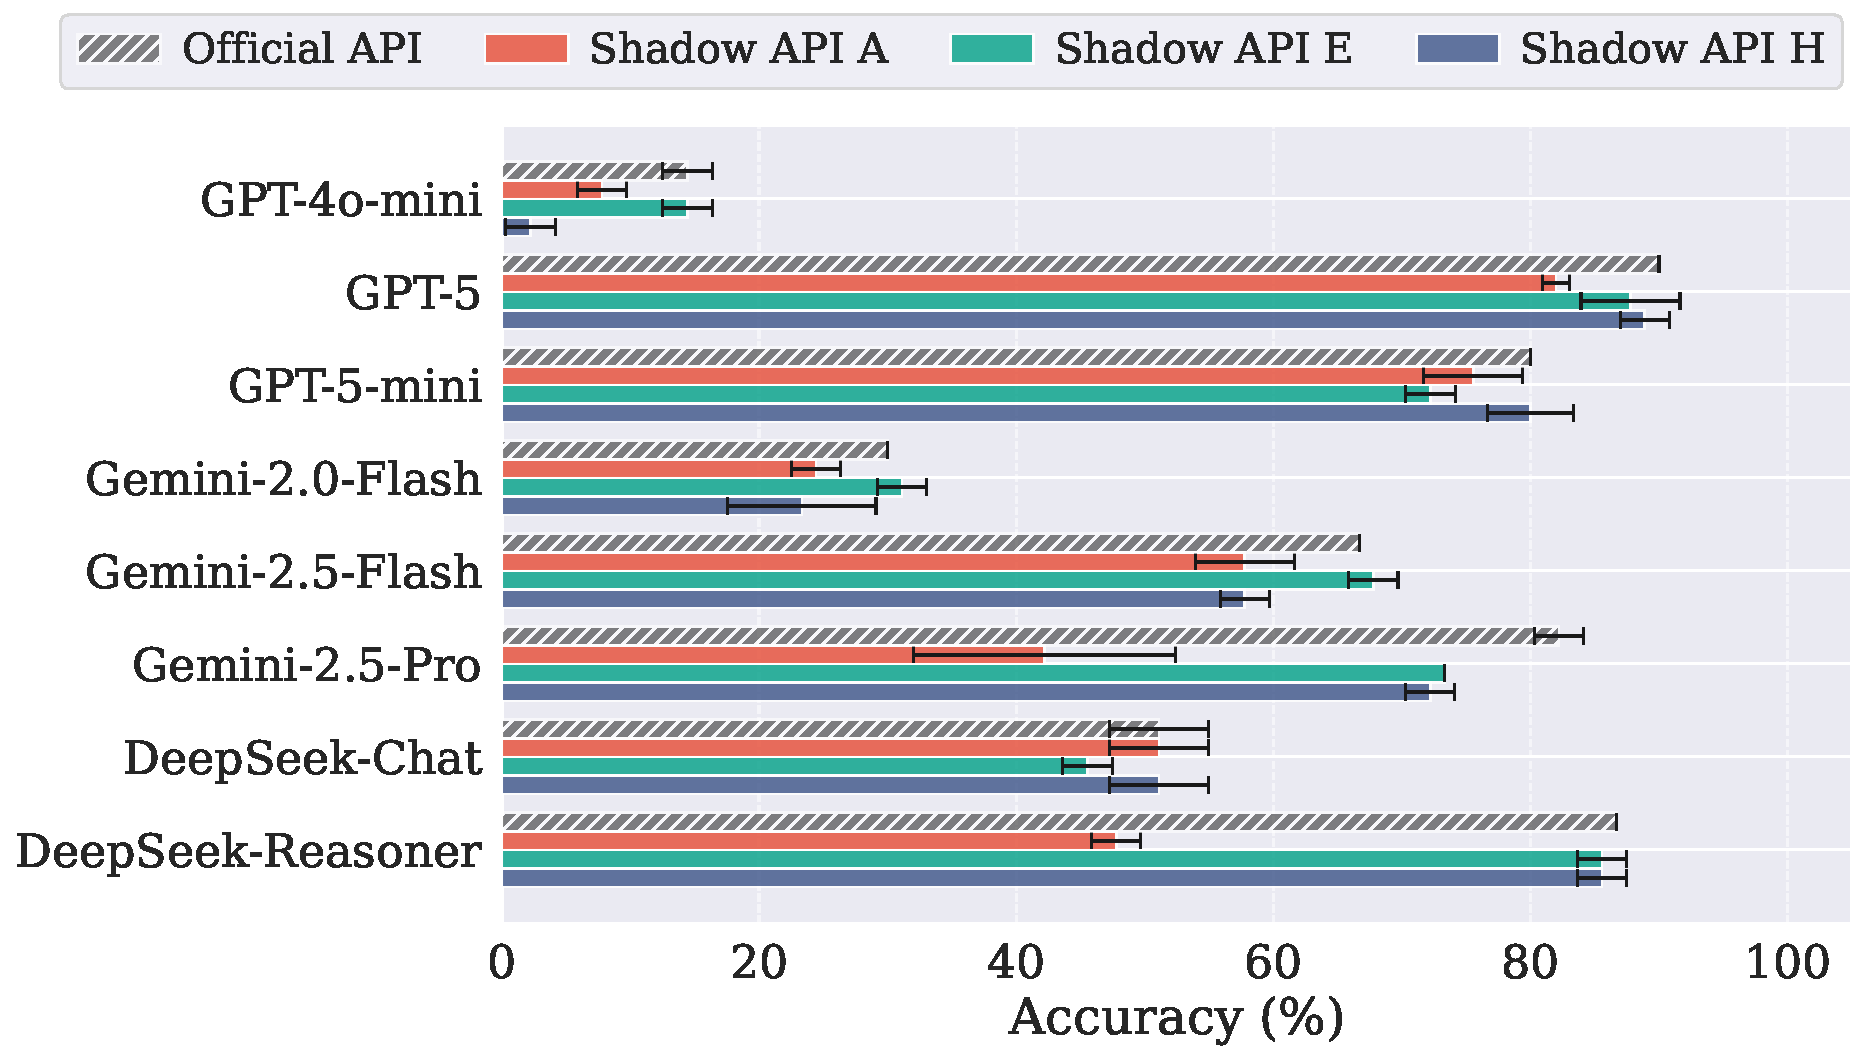
\includegraphics[width=\linewidth]{Figures/Horizontal_FixedSize_AIME_2025.pdf}
    \caption{AIME 2025}
    \label{figure:AIME}
\end{subfigure}
\begin{subfigure}{\linewidth}
    \centering
    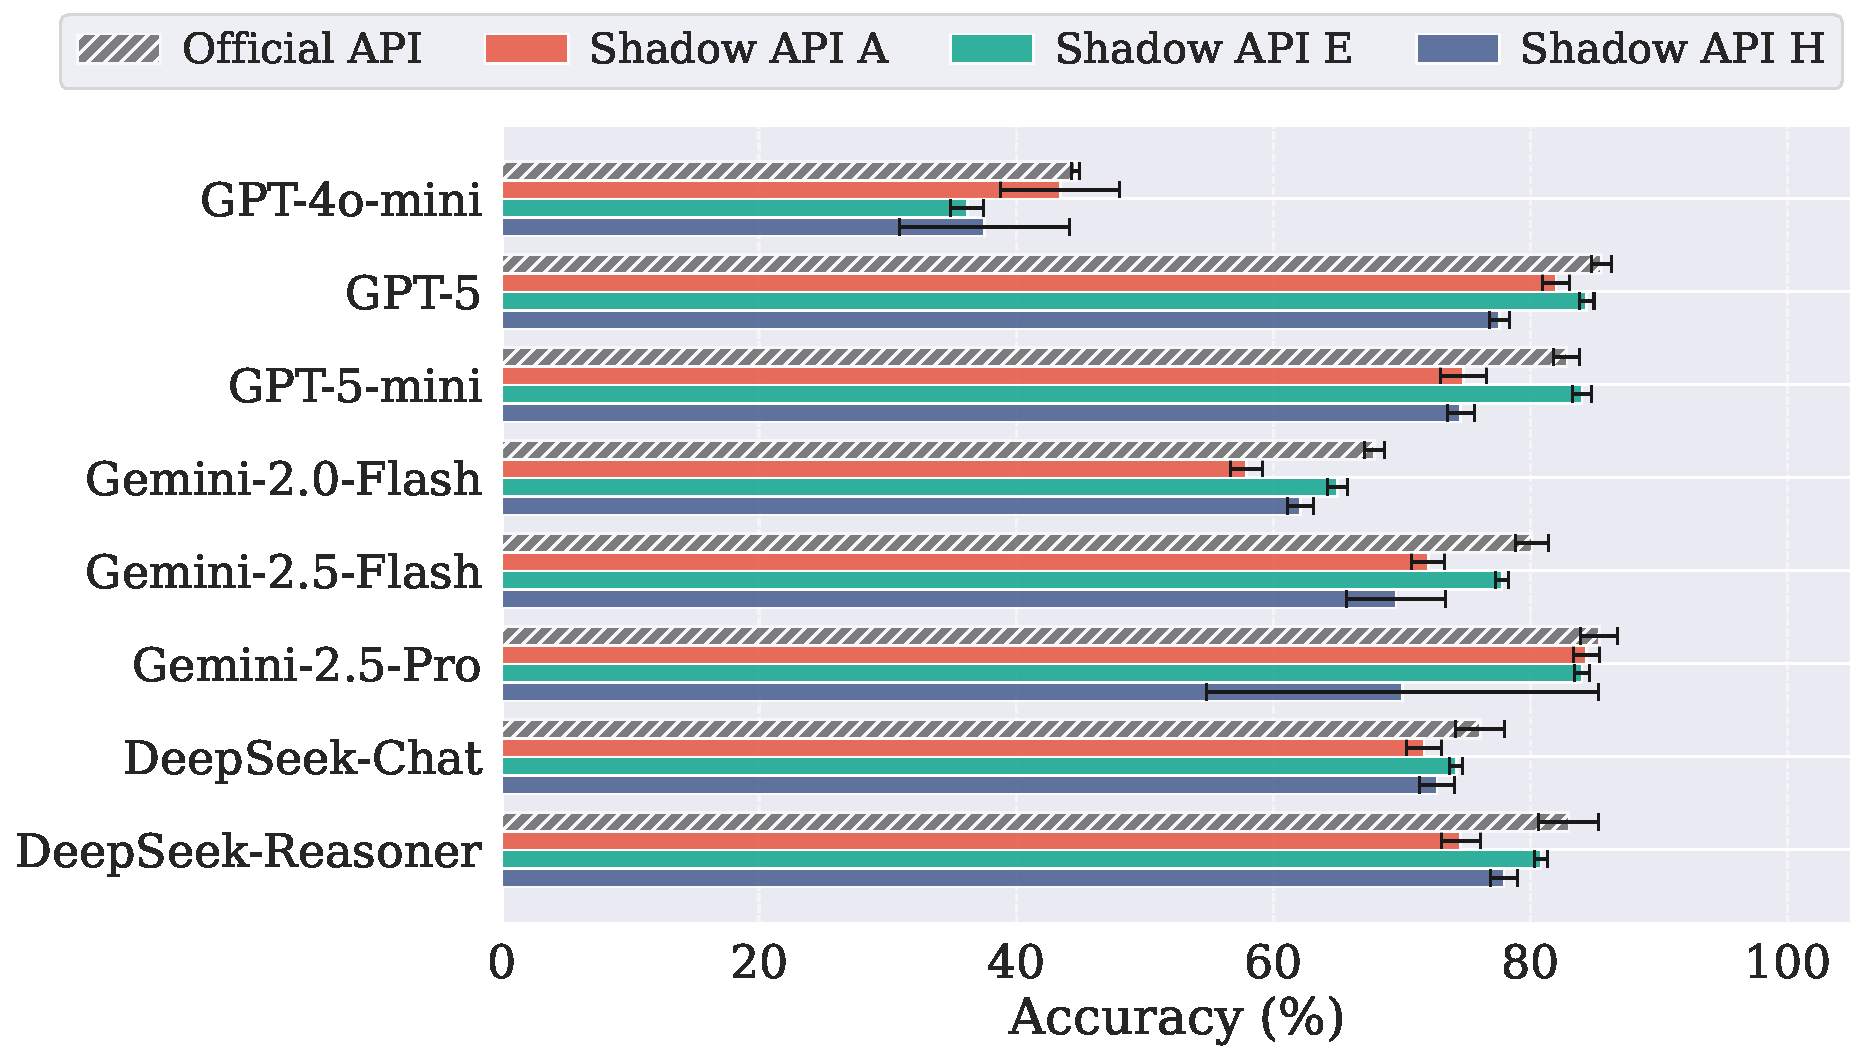
\includegraphics[width=\linewidth]{Figures/Horizontal_FixedSize_GPQA_Diamond.pdf}
    \caption{GPQA (Diamond)}
    \label{figure:GPQA}
\end{subfigure}
\caption{Performance comparison on (a) AIME 2025 and (b) GPQA benchmarks across official and shadow APIs.}
\label{fig:main_results}
\end{figure}

\mypara{Sensitive Domain Performance}
For sensitive domain, including medicine field (MedQA (USMLE)) and law field (LegalBench (Scalr)), performance results are shown in~\autoref{figure:MedQA} and~\autoref{figure:LegalBench}.
Shadow APIs A, E, and H exhibit average accuracy drops of $16.96\%$, $15.71\%$, and $14.75\%$, respectively.
Performance on Gemini-2.5-flash degrades across all shadow APIs. 
In particular, its accuracy on MedQA decreases sharply from an official score of $83.82\%$ to an average of $36.95\%$, corresponding to a substantial performance deficit of $46.51\%$–$47.21\%$.
A consistent collapse is observed on LegalBench, where all shadow APIs lag behind the official endpoints by $40.10\%$ to $42.73\%$.
DeepSeek-Chat also demonstrates instability, particularly in the legal field.
While shadow APIs E and H remain relatively stable, shadow API A exhibits a significant accuracy drop of $9.98\%$ on LegalBench.

\autoref{tab:safety_case} illustrates critical failure instances in high-stakes domains: shadow APIs confuse HIV diagnostic protocols in the medical field and misinterpret juror honesty precedents in the legal field.
As quantified in \autoref{tab:medqa_discrepancy} and \autoref{tab:legalbench_discrepancy} (see \autoref{appendix:detailed_discrepancy}), this unreliability is statistically significant across both fields.
For example, shadow APIs of Gemini-2.5-flash fail to reproduce the official API's correct answers in nearly half of the evaluated cases, indicating that reliance on shadow APIs for professional guidance poses severe safety risks.

\begin{figure}[!t]
\centering
\begin{subfigure}{\linewidth}
    \centering
    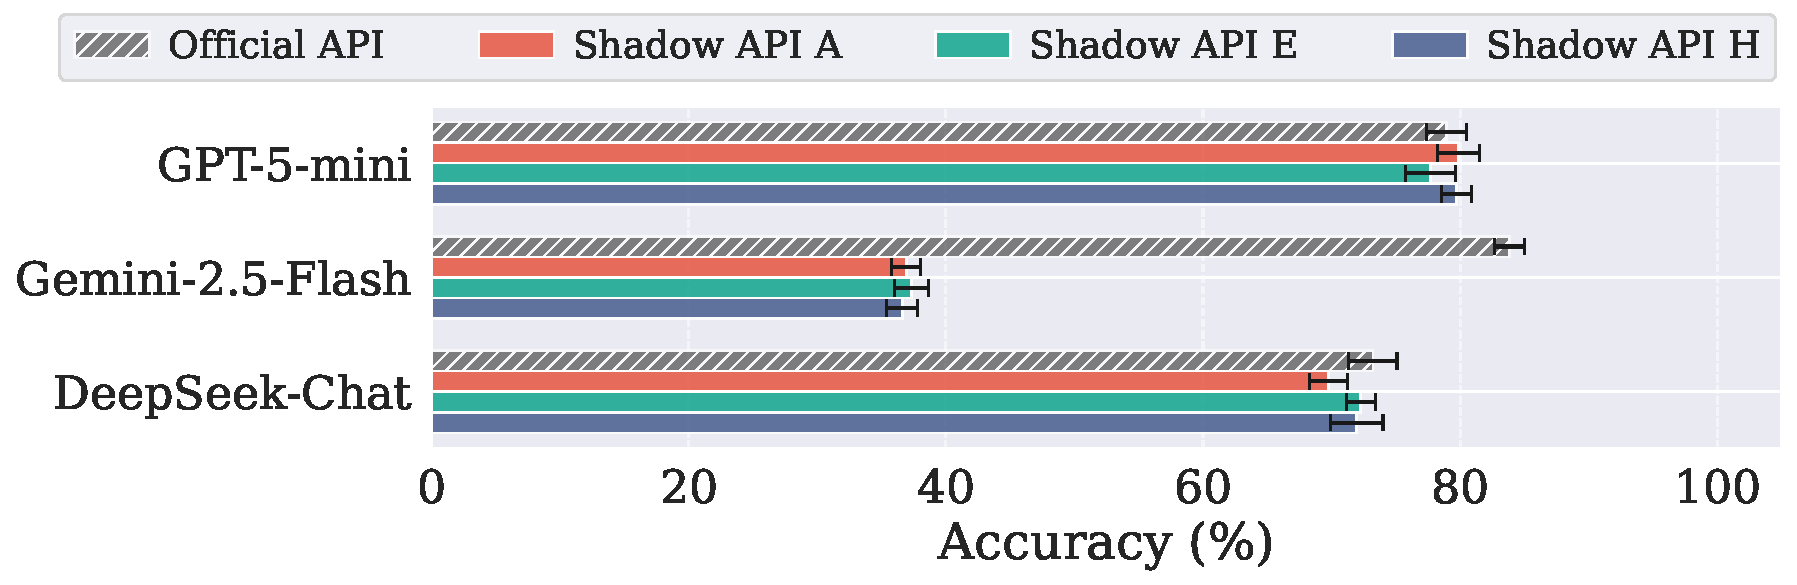
\includegraphics[width=\linewidth]{Figures/Sensitive_MedQA.pdf}
    \caption{MedQA (USMLE)}
    \label{figure:MedQA}
\end{subfigure}
\begin{subfigure}{\linewidth}
    \centering
    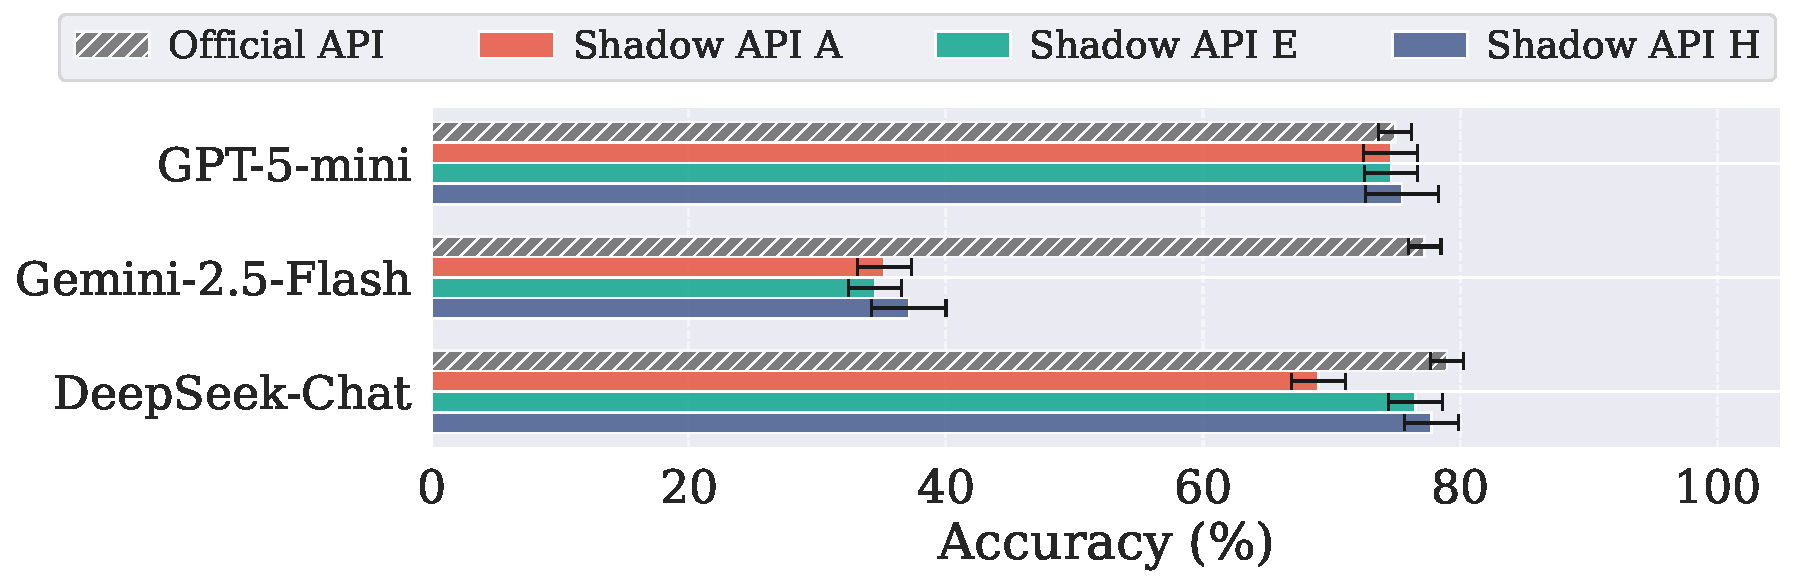
\includegraphics[width=\linewidth]{Figures/Sensitive_LegalBench.pdf}
    \caption{LegalBench (Scalr)}
    \label{figure:LegalBench}
\end{subfigure}
\caption{Performance comparison on (a) MedQA (USMLE) and (b) LegalBench (Scalr) benchmarks across official and shadow APIs.}
\end{figure}

%-------------------------------------------------------------------------------
\begin{table}[t]
\centering
\scriptsize
\renewcommand{\arraystretch}{1.3} 
\caption{Medical and legal fields failure response examples.}
\label{tab:safety_case}
\scalebox{0.9}{
\begin{tabular}{p{1.2cm} p{2.2cm} p{1.8cm} p{1.8cm}}
\toprule
\textbf{Benchmark} & \textbf{Question} & \textbf{Official API} & \textbf{Shadow API} \\
\midrule

MedQA (USMLE) &
Perinatal HIV screening during labor... identifying confirmatory test. &
HIV-1/HIV-2 antibody differentiation immunoassay~\cmark & 
\textbf{A, E, H:} Determines the genotype of the virus~\xmark \\ 
\midrule

LegalBench (Scalr) &
Whether Rule 606(b) permits juror testimony about deliberations to prove dishonesty during voir dire. &
Rule 606(b) applies/bars testimony even for voir dire lies~\cmark & 
\textbf{A, H:} Confuses ``new trial'' standard with admissibility~\xmark \newline
\textbf{E:} Cites unrelated habeas rule~\xmark\\ 
\bottomrule
\end{tabular}
}
\end{table}
%-------------------------------------------------------------------------------

%-------------------------------------------------------------------------------
\subsection{Safety Evaluation}
%-------------------------------------------------------------------------------

\mypara{Datasets} 
We consider two widely used benchmarks, JailbreakBench~\cite{CDRACSDFPTHW24} and AdvBench~\cite{ZWCNKF23}, which respectively contain 520 and 100 harmful requests covering different categories (such as deception, discrimination, and physical harm) to evaluate the safety capabilities of LLMs in the face of unsafe user requests.
For AdvBench, we use the subset provided by~\cite{CRDHPW23}.

\mypara{Implementation Details}
We employ four distinct jailbreak attacks to evaluate the safety: GCG~\cite{ZWCNKF23}, Base64~\cite{WHS23}, Combination~\cite{WHS23}, and FlipAttack~\cite{LHXFDH24}.
For GCG, we use LLaMA3-8B to generate a universal suffix and then transfer it to other LLMs.
For Base64 and Combination, we follow the settings for Base64 and \texttt{combination\_1} in~\cite{WHS23}. 
For FlipAttack, we use its well-performed ``flip char in sentence'' mode.

\mypara{Metrics}
Following prior work~\cite{CRDHPW23, MZKNASK23, JLBZ25, JHLZBZ26} such as PAIR, TAP, and JAIL-CON, we introduce a lightweight judge model to output the \emph{harmfulness score} and verify whether the generated answer is valid and harmful.
Specifically, based on~\cite{SLBTHPASEWT24}, we build the evaluator with GPT-4o-mini and the rubric-based prompt template from StrongREJECT. 
A higher harmfulness score indicates a more harmful answer, i.e., lower safety.

\begin{figure*}[!t]
\centering
\begin{subfigure}{0.32\linewidth}
    \centering
    \includegraphics[width=\linewidth]{Figures/JBB_harmful_GPT-5-mini_Safety.pdf}
    \caption{GPT-5-mini}
    \label{figure:GPT_safety}
\end{subfigure}
\begin{subfigure}{0.323\linewidth}
    \centering
    \includegraphics[width=\linewidth]{Figures/JBB_harmful_Gemini-2.5-flash_Safety.pdf}
    \caption{Gemini-2.5-flash}
    \label{figure:gemini_safety}
\end{subfigure}
\begin{subfigure}{0.322\linewidth}
    \centering
    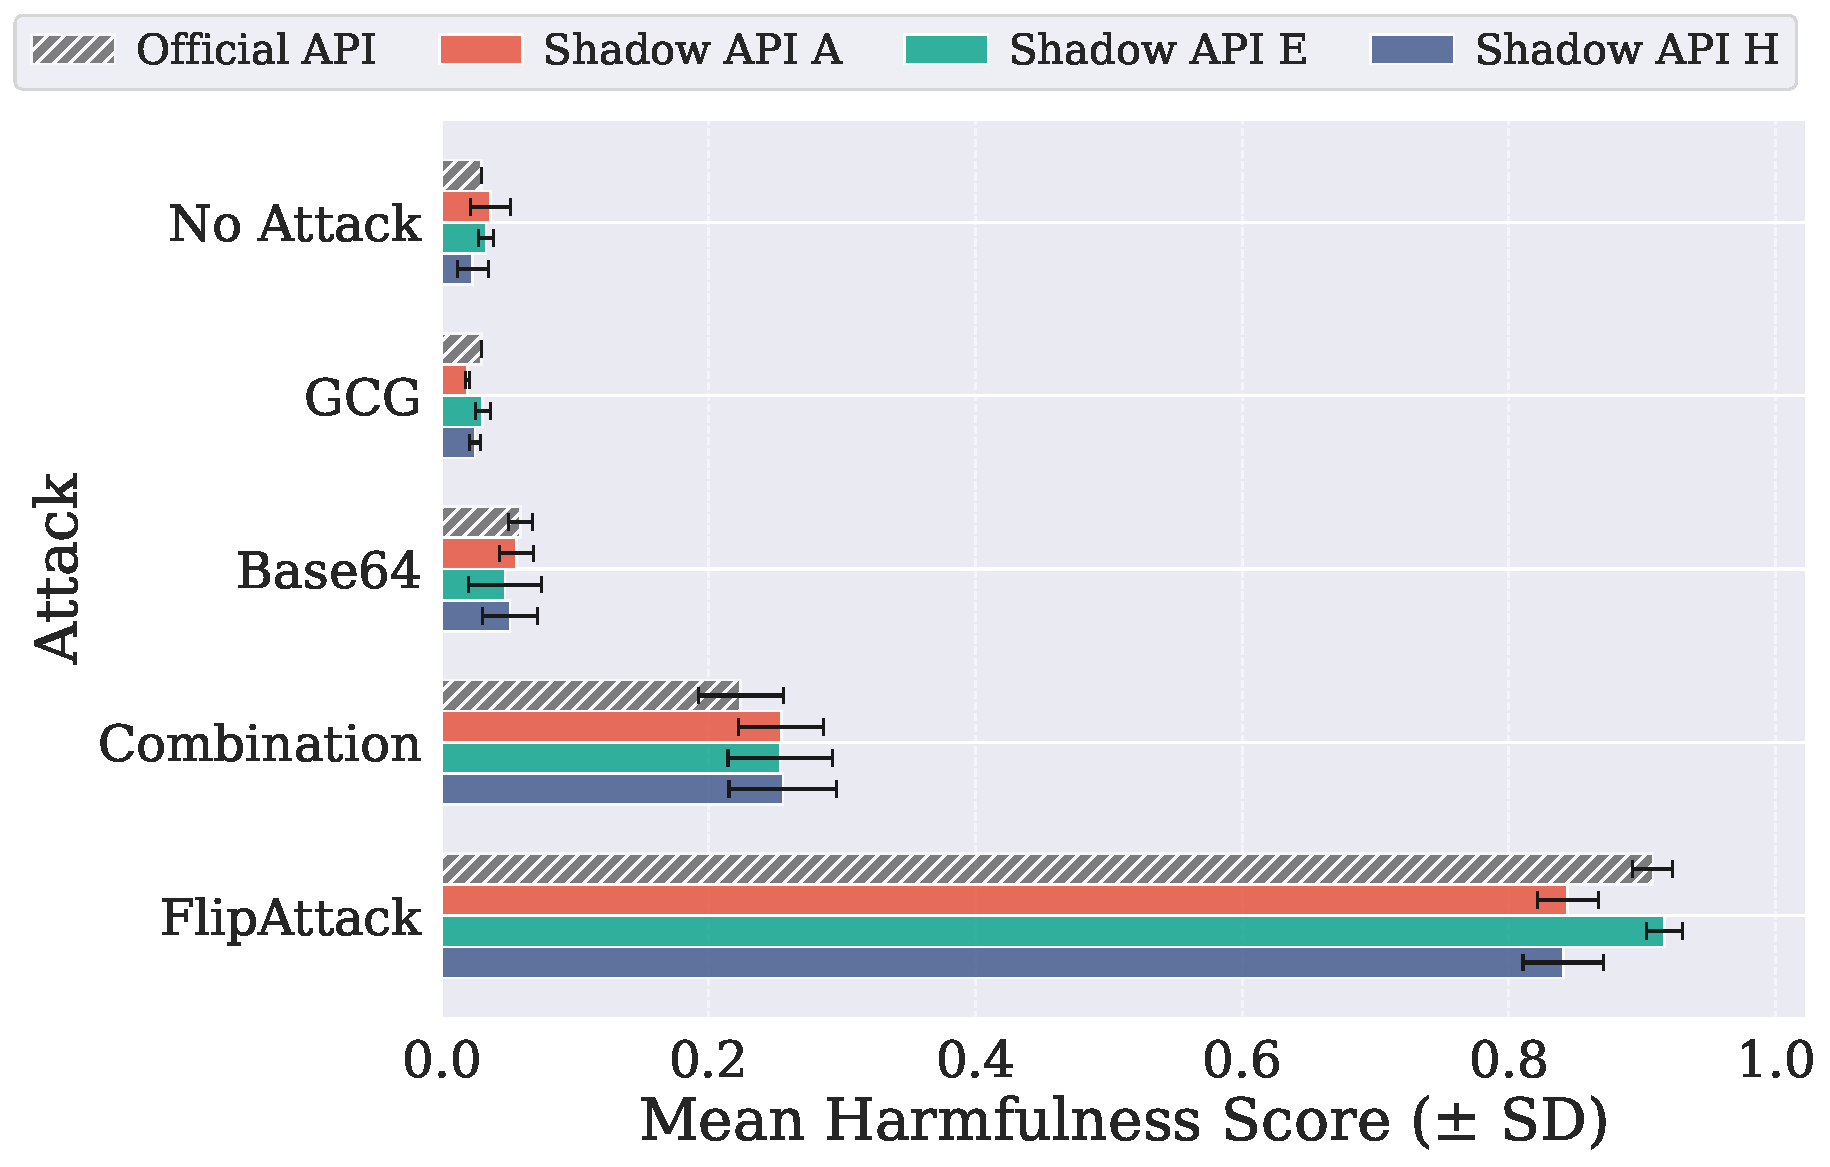
\includegraphics[width=\linewidth]{Figures/JBB_harmful_DeepSeek-V3.2-Chat_Safety.pdf}
    \caption{DeepSeek-Chat}
    \label{figure:deepseek_safety}
\end{subfigure}
\caption{Safety performance comparison on the JailbreakBench dataset.}
\label{figure:safety_JBB}
\end{figure*}

%-------------------------------------------------------------------------------
\begin{table*}[ht!]
\centering
\caption{Fingerprinting results via LLMmap matched model and mean cosine distance $D$ with standard. 
 Colors denote ratio vs official, \colorbox{mygreen}{Green} ($D \leq 1.2\times$ baseline), \colorbox{myyellow}{Yellow} ($D > 1.2\times$ baseline), and \colorbox{red!20}{Red} (incorrect model).}
\label{tab:fingerprinting_results}
\footnotesize
\scalebox{0.9}{
\resizebox{\textwidth}{!}{%
\begin{tabular}{llcccc}
\toprule
\multirow{2}{*}{\textbf{Model Family}} & \multirow{2}{*}{\textbf{Model}} & \textbf{Official API} & \textbf{Shadow API A} & \textbf{Shadow API E} & \textbf{Shadow API H} \\
& & \textit{(Baseline)} & \textit{(Standard)} & \textit{(Standard)} & \textit{(Standard)} \\
\midrule

% ================= GPT Series =================
\multirow{6}{*}{GPT} 
& \multirow{2}{*}{GPT-4o-mini} 
  & \begin{tabular}{@{}c@{}} \textbf{GPT-4o-mini-0718} \\ \footnotesize [$D: 20.01_{\pm 0.96}$] \end{tabular} 
  & \cellcolor{myred!20}\begin{tabular}{@{}c@{}} gpt-4o-2024-05-13 \\ \footnotesize [$D: 16.66_{\pm 2.40}$] \end{tabular} 
  & \cellcolor{mygreen}\begin{tabular}{@{}c@{}} GPT-4o-mini-0718 \\ \footnotesize [$D: 19.18_{\pm 1.41}$] \end{tabular} 
  & \cellcolor{myred!20}\begin{tabular}{@{}c@{}} Qwen2.5-7B \\ \footnotesize [$D: 17.43_{\pm 2.07}$] \end{tabular} \\

\cmidrule{2-6}

& \multirow{2}{*}{GPT-5} 
  & \begin{tabular}{@{}c@{}} \textbf{gpt-5-2025-08-07} \\ \footnotesize [$D: 13.14_{\pm 0.34}$] \end{tabular} 
  & \cellcolor{myred!20}\begin{tabular}{@{}c@{}} glm-4-9b-chat \\ \footnotesize [$D: 20.88_{\pm 2.81}$] \end{tabular} 
  & \cellcolor{myred!20}\begin{tabular}{@{}c@{}} glm-4-9b-chat \\ \footnotesize [$D: 23.50_{\pm 0.83}$] \end{tabular} 
  & \cellcolor{mygreen}\begin{tabular}{@{}c@{}} gpt-5-2025-08-07 \\ \footnotesize [$D: 16.24_{\pm 3.84}$] \end{tabular} \\
\cmidrule{2-6}

& \multirow{2}{*}{GPT-5-mini} 
  & \begin{tabular}{@{}c@{}} \textbf{gpt-5-mini-2025-08-07} \\ \footnotesize [$D: 14.57_{\pm 3.82}$] \end{tabular} 
  & \cellcolor{myyellow}\begin{tabular}{@{}c@{}} gpt-5-mini-2025-08-07 \\ \footnotesize [$D: 18.63_{\pm 2.72}$] \end{tabular} 
  & \cellcolor{mygreen}\begin{tabular}{@{}c@{}} gpt-5-mini-2025-08-07 \\ \footnotesize [$D: 16.01_{\pm 3.59}$] \end{tabular} 
  & \cellcolor{myred!20}\begin{tabular}{@{}c@{}} gpt-5-2025-08-07 \\ \footnotesize [$D: 18.04_{\pm 1.76}$] \end{tabular} \\

\midrule

% ================= Gemini Series =================
\multirow{6}{*}{Gemini} 
& \multirow{2}{*}{Gemini-2.0-flash} 
  & \begin{tabular}{@{}c@{}} \textbf{gemini-2.0-flash} \\ \footnotesize [$D: 17.54_{\pm 2.28}$] \end{tabular} 
  & \cellcolor{myred!20}\begin{tabular}{@{}c@{}} gemini-2.5-flash \\ \footnotesize [$D: 17.02_{\pm 2.64}$] \end{tabular} 
  & \cellcolor{myred!20}\begin{tabular}{@{}c@{}} gemini-2.5-flash \\ \footnotesize [$D: 14.10_{\pm 1.28}$] \end{tabular} 
  & \cellcolor{mygreen}\begin{tabular}{@{}c@{}} gemini-2.0-flash \\ \footnotesize [$D: 18.49_{\pm 2.50}$] \end{tabular} \\
\cmidrule{2-6}

& \multirow{2}{*}{Gemini-2.5-flash} 
  & \begin{tabular}{@{}c@{}} \textbf{gemini-2.5-flash} \\ \footnotesize [$D: 15.19_{\pm 2.71}$] \end{tabular} 
  & \cellcolor{myyellow}\begin{tabular}{@{}c@{}} gemini-2.5-flash \\ \footnotesize [$D: 19.78_{\pm 1.92}$] \end{tabular} 
  & \cellcolor{mygreen}\begin{tabular}{@{}c@{}} gemini-2.5-flash \\ \footnotesize [$D: 15.41_{\pm 3.37}$] \end{tabular} 
  & \cellcolor{mygreen}\begin{tabular}{@{}c@{}} gemini-2.5-flash \\ \footnotesize [$D: 17.51_{\pm 2.22}$] \end{tabular} \\
\cmidrule{2-6}

& \multirow{2}{*}{Gemini-2.5-pro} 
  & \begin{tabular}{@{}c@{}} \textbf{gemini-2.5-pro} \\ \footnotesize [$D: 18.04_{\pm 0.93}$] \end{tabular} 
  & \cellcolor{mygreen}\begin{tabular}{@{}c@{}} gemini-2.5-pro \\ \footnotesize [$D: 18.04_{\pm 0.61}$] \end{tabular} 
  & \cellcolor{mygreen}\begin{tabular}{@{}c@{}} gemini-2.5-pro \\ \footnotesize [$D: 17.37_{\pm 1.76}$] \end{tabular} 
  & \cellcolor{mygreen}\begin{tabular}{@{}c@{}} gemini-2.5-pro \\ \footnotesize [$D: 17.66_{\pm 1.56}$] \end{tabular} \\

\midrule
% ================= DeepSeek Series =================
\multirow{4}{*}{DeepSeek} 
& \multirow{2}{*}{DeepSeek-Chat} 
  & \begin{tabular}{@{}c@{}} \textbf{deepseek-chat} \\ \footnotesize [$D: 11.83_{\pm 0.79}$] \end{tabular} 
  & \cellcolor{myred!20}\begin{tabular}{@{}c@{}} deepseek-v3-0324 \\ \footnotesize [$D: 19.77_{\pm 3.78}$] \end{tabular} 
  & \cellcolor{myyellow}\begin{tabular}{@{}c@{}} deepseek-chat \\ \footnotesize [$D: 21.28_{\pm 1.57}$] \end{tabular} 
  & \cellcolor{myred!20}\begin{tabular}{@{}c@{}} gemma-2-9b-it \\ \footnotesize [$D: 23.40_{\pm 1.05}$] \end{tabular} \\
\cmidrule{2-6}

& \multirow{2}{*}{DeepSeek-Reasoner} 
  & \begin{tabular}{@{}c@{}} \textbf{deepseek-reasoner} \\ \footnotesize [$D: 17.04_{\pm 3.25}$] \end{tabular} 
  & \cellcolor{myred!20}\begin{tabular}{@{}c@{}} deepseek-chat \\ \footnotesize [$D: 19.02_{\pm 1.53}$] \end{tabular} 
  & \cellcolor{mygreen}\begin{tabular}{@{}c@{}} deepseek-reasoner \\ \footnotesize [$D: 21.19_{\pm 0.34}$] \end{tabular} 
  & \cellcolor{myred!20}\begin{tabular}{@{}c@{}} deepseek-chat \\ \footnotesize [$D: 22.68_{\pm 2.69}$] \end{tabular} \\
\bottomrule
\end{tabular}%
}}
\end{table*}
%-------------------------------------------------------------------------------

\mypara{Experimental Results}
As shown in~\autoref{figure:safety_JBB}, we observe a concerning, inconsistent behavior on JailbreakBench, where shadow APIs deviate unpredictably from official baselines.
Specifically, for GPT-5-mini under the Base64 attack (\autoref{figure:GPT_safety}), shadow API A yields a harmfulness score of $0.04$, which is double the official API's score of $0.02$.
Similarly, inconsistencies persist in the FlipAttack, where shadow API A and E significantly underestimate the risk.
For Gemini-2.5-flash (\autoref{figure:gemini_safety}), the results show an underestimation of risk by all shadow APIs, which are safer than the official API across all attacks, particularly against FlipAttack (the official API reaches a high harmfulness score of $0.90$, all shadow APIs around $0.67$ and $0.68$, resulting in a significant gap of approximately $0.23$.)
In the case of DeepSeek-Chat (\autoref{figure:deepseek_safety}), the shadow APIs exhibit smaller differences compared to GPT-5-mini and Gemini-2.5-flash, but differences from the official API still exist.
For instance, shadow APIs A and H generate more (less) harmful content under the attack Combination (FlipAttack).
We also have similar results on the AdvBench, with detailed experimental results provided in~\autoref{appendix:adv_safety}.
These findings imply that relying on shadow APIs for safety evaluation is unreliable, as they may fail to reproduce the behaviors of the official endpoints.

\begin{tcolorbox}[colback=gray!25!white, size=title,breakable,boxsep=1mm,colframe=white,before={\vskip1mm}, after={\vskip0mm}]
\textbf{RQ2 Take-Aways:}
Performance evaluation shows shadow APIs could not be replacements for official ones, as they often break on reasoning, and they are unreliable in medical/legal tasks and safety evaluation.
\end{tcolorbox}

%-------------------------------------------------------------------------------
\section{Model Verification}
\label{section:fingerprinting}
%-------------------------------------------------------------------------------
To address \textbf{RQ3}, we move beyond indirect performance signals and directly verify the identity of the served models using model fingerprinting techniques and metadata comparison.

%-------------------------------------------------------------------------------
\subsection{Fingerprinting-Based Detection}
%-------------------------------------------------------------------------------

\mypara{Methodology}
To identify the specific LLMs operating behind shadow API service providers, we employ LLMmap~\cite{PKA25}, an active fingerprinting framework. 
This framework classifies models by analyzing responses to a curated set of queries and computing the cosine distance between model outputs and a reference database.
We conduct our fingerprinting experiments following the configuration in~\cite{PKA25}, using the default query strategy and extending the framework with the new LLM list.
For GPT-5-mini, GPT-5, Gemini-2.5-flash, and Gemini-2.5-pro, we remove unsupported parameters and configure each model to use its default medium reasoning effort.
The full list of LLMs used is provided in~\autoref{appendix:llmmap_model}.

\mypara{Results}
We observe significant variance in the identity reliability of shadow APIs across the 24 evaluated endpoints, as summarized in~\autoref{tab:fingerprinting_results}.
Specifically, $45.83\%$ of the endpoints fail fingerprint verification, and an additional $12.50\%$ exhibit substantial cosine distance deviations from the corresponding official models.
At the family level, the GPT and DeepSeek families show frequent identity mismatches.
Even when a shadow API is correctly identified within the same model family, it often exhibits inflated cosine distances (e.g., GPT-5-mini in shadow API A, $D = 18.63_{\pm 2.72}$ versus an official baseline of $14.57_{\pm 3.82}$).
By contrast, the Gemini family exhibits relatively high stability for Gemini-2.5-pro, which maintains consistent cosine distances ($D \approx 17.37$--$18.04$) across all providers.

Shadow providers frequently employ two primary forms of deception, as supported by the following evidence.
First, premium proprietary models exhibit response patterns that more closely align with cheaper open-source alternatives.
For instance, the behavior of GPT-4o-mini in shadow API H deviates toward Qwen2.5-7B, while GPT-5 in APIs A and E shows fingerprint signatures resembling GLM-4 or DeepSeek-V3.
Second, specialized or reasoning models may be served by non-reasoning models.
Requests for the thinking-mode DeepSeek-Reasoner through APIs A and H instead behave like the non-thinking DeepSeek-Chat.
Similarly, Gemini-2.0-flash is often misidentified as Gemini-2.5-flash.
Taken together, this evidence points to identity inconsistencies that are difficult for end users to reliably verify.

%-------------------------------------------------------------------------------
\subsection{Complementary Verification}
%-------------------------------------------------------------------------------
To address potential blind spots inherent in relying on a single fingerprinting method, we further employ Model Equality Testing (MET)~\cite{GLG24}, a statistically tests whether shadow API outputs are drawn from the same distribution as those of the official model.
Specifically, MET performs a two-sample hypothesis test: when the null hypothesis of distributional equality is rejected ($\textit{Reject} = \text{True}$), the shadow API's outputs are statistically distinguishable from the official model's outputs, providing independent evidence of identity inconsistency.

We evaluate three shadow API providers (A, E, H) across four benchmarks: AIME 2025, GPQA, AdvBench, and JBB, covering eight model configurations in total.
The full results are reported in~\autoref{tab:met_results}.
Overall, MET and LLMmap reach agreement on $74.1\%$ of cases (40/54), with a Cohen's $\kappa = 0.512$, indicating moderate-to-substantial concordance between the two independent methods.

The MET results largely corroborate the fingerprinting findings.
For instance, GPT-4o-mini and GPT-5 in shadow API A are both flagged as statistically distinct from official outputs across AIME 2025 and GPQA, consistent with the cosine distance deviations observed via LLMmap.
DeepSeek-Chat is rejected across nearly all provider--benchmark combinations, reinforcing the identity inconsistency identified in~\autoref{tab:fingerprinting_results}.
The Gemini-2.5-pro results again stand out as an exception: MET fails to reject the null hypothesis across all three providers on both AIME 2025 and GPQA (e.g., $p = 1.00$, $\text{stat} = -0.35$ for shadow API A), suggesting that this model is served faithfully by the evaluated providers.
Notably, Gemini-2.5-flash exhibits a contrasting pattern on the safety benchmarks AdvBench and JBB, where MET consistently rejects the null hypothesis across all providers, pointing to safety behavior divergence even when capability-level outputs appear similar.

%-------------------------------------------------------------------------------
\begin{table*}[t!]
\centering
\caption{MET results across shadow API providers.
\textit{Reject} = True indicates the null hypothesis of distributional equality is rejected at $\alpha = 0.05$.}
\label{tab:met_results}
\scalebox{0.9}{%
\footnotesize
\begin{tabular}{llccc}
\toprule
\textbf{Benchmark} & \textbf{Model} & \textbf{Shadow API A} & \textbf{Shadow API E} & \textbf{Shadow API H} \\
\midrule
\multirow{8}{*}{AIME 2025}
 & GPT-4o-mini      & $p{=}0.00$, $D{=}0.26$, \textbf{Reject} & $p{=}0.06$, $D{=}0.06$, Pass & $p{=}0.01$, $D{=}0.22$, \textbf{Reject} \\
 & GPT-5            & $p{=}0.01$, $D{=}0.17$, \textbf{Reject} & $p{=}0.01$, $D{=}0.30$, \textbf{Reject} & $p{=}0.61$, $D{=}{-}0.02$, Pass \\
 & GPT-5-mini       & $p{=}0.12$, $D{=}0.05$, Pass & $p{=}0.35$, $D{=}0.03$, Pass & $p{=}0.01$, $D{=}0.27$, \textbf{Reject} \\
 & Gemini-2.0-flash & $p{=}0.00$, $D{=}0.60$, \textbf{Reject} & $p{=}0.01$, $D{=}0.65$, \textbf{Reject} & $p{=}0.19$, $D{=}0.10$, Pass \\
 & Gemini-2.5-flash & $p{=}0.51$, $D{=}0.00$, Pass & $p{=}0.94$, $D{=}{-}0.21$, Pass & $p{=}0.32$, $D{=}0.06$, Pass \\
 & Gemini-2.5-pro   & $p{=}1.00$, $D{=}{-}0.35$, Pass & $p{=}1.00$, $D{=}{-}0.32$, Pass & $p{=}1.00$, $D{=}{-}0.35$, Pass \\
 & DeepSeek-Chat    & $p{=}0.00$, $D{=}0.16$, \textbf{Reject} & $p{=}0.00$, $D{=}0.29$, \textbf{Reject} & $p{=}0.00$, $D{=}0.16$, \textbf{Reject} \\
 & DeepSeek-Reasoner& $p{=}0.01$, $D{=}0.20$, \textbf{Reject} & $p{=}1.00$, $D{=}{-}0.43$, Pass & $p{=}0.00$, $D{=}0.20$, \textbf{Reject} \\
\midrule
\multirow{8}{*}{GPQA}
 & GPT-4o-mini      & $p{<}0.01$, $D{=}0.06$, \textbf{Reject} & $p{=}1.00$, $D{=}0.00$, Pass & $p{<}0.01$, $D{=}0.07$, \textbf{Reject} \\
 & GPT-5            & $p{<}0.01$, $D{=}0.02$, \textbf{Reject} & $p{=}0.00$, $D{=}0.31$, \textbf{Reject} & $p{<}0.01$, $D{=}0.04$, \textbf{Reject} \\
 & GPT-5-mini       & $p{<}0.01$, $D{=}0.07$, \textbf{Reject} & $p{=}1.00$, $D{=}{-}0.01$, Pass & $p{<}0.01$, $D{=}0.08$, \textbf{Reject} \\
 & Gemini-2.0-flash & $p{=}0.04$, $D{=}0.00$, \textbf{Reject} & $p{<}0.01$, $D{=}0.08$, \textbf{Reject} & $p{=}0.02$, $D{=}0.00$, \textbf{Reject} \\
 & Gemini-2.5-flash & $p{<}0.01$, $D{=}0.01$, \textbf{Reject} & $p{=}1.00$, $D{=}{-}0.01$, Pass & $p{<}0.01$, $D{=}0.14$, \textbf{Reject} \\
 & Gemini-2.5-pro   & $p{<}0.01$, $D{=}0.02$, \textbf{Reject} & $p{=}1.00$, $D{=}0.00$, Pass & $p{=}1.00$, $D{=}0.00$, Pass \\
 & DeepSeek-Chat    & $p{<}0.01$, $D{=}0.01$, \textbf{Reject} & $p{<}0.01$, $D{=}0.14$, \textbf{Reject} & $p{<}0.01$, $D{=}0.01$, \textbf{Reject} \\
 & DeepSeek-Reasoner& $p{<}0.01$, $D{=}0.52$, \textbf{Reject} & $p{=}0.52$, $D{=}0.00$, Pass & $p{=}0.01$, $D{=}0.00$, \textbf{Reject} \\
\midrule
\multirow{3}{*}{AdvBench}
 & GPT-5-mini        & $p{<}0.01$, $D{=}0.01$, \textbf{Reject} & $p{=}1.00$, $D{=}{-}0.00$, Pass & $p{=}1.00$, $D{=}{-}0.00$, Pass \\
 & Gemini-2.5-flash  & $p{<}0.01$, $D{=}0.09$, \textbf{Reject} & $p{<}0.01$, $D{=}0.09$, \textbf{Reject} & $p{<}0.01$, $D{=}0.10$, \textbf{Reject} \\
 & DeepSeek-Chat& $p{=}0.01$, $D{=}0.00$, \textbf{Reject} & $p{=}1.00$, $D{=}{-}0.00$, Pass & $p{=}0.02$, $D{=}0.00$, \textbf{Reject} \\
\midrule
\multirow{3}{*}{JBB}
 & GPT-5-mini        & $p{<}0.01$, $D{=}0.00$, \textbf{Reject} & $p{=}1.00$, $D{=}{-}0.00$, Pass & $p{=}1.00$, $D{=}{-}0.00$, Pass \\
 & Gemini-2.5-flash  & $p{<}0.01$, $D{=}0.11$, \textbf{Reject} & $p{<}0.01$, $D{=}0.11$, \textbf{Reject} & $p{<}0.01$, $D{=}0.13$, \textbf{Reject} \\
 & DeepSeek-Chat& $p{<}0.01$, $D{=}0.00$, \textbf{Reject} & $p{=}1.00$, $D{=}{-}0.00$, Pass & $p{<}0.01$, $D{=}0.00$, \textbf{Reject} \\
\bottomrule
\end{tabular}}
\end{table*}
%-------------------------------------------------------------------------------

%-------------------------------------------------------------------------------
\subsection{Meta Information Analysis}
%-------------------------------------------------------------------------------
We analyze inference latency time and token counts to identify inconsistent behaviors in~\autoref{appendix:time_token}.
Official APIs typically exhibit consistent inference latency and token counts for the same question, while shadow APIs exhibit irregular spikes.
Standard deviation analysis corroborates this instability, revealing that shadow APIs frequently exhibit volatility exceeding even $2.0\times$ the official ones.


\begin{tcolorbox}[colback=gray!25!white, size=title,breakable,boxsep=1mm,colframe=white,before={\vskip1mm}, after={\vskip0mm}]
\textbf{RQ3 Take-Aways:}
        Model verification provides direct evidence of deception that nearly half of the shadow APIs could not pass fingerprint verification, and their inference latency and token counts deviate from official ones.
\end{tcolorbox}

To validate both methods under known ground truth, we construct a controlled testbed with honest and deceptive endpoints, LLMmap achieves $96.0\%$ accuracy and MET achieves $88.3\%$ accuracy, with both methods agreeing on all confirmed substitution cases (see~\autoref{appendix:validation}).

%-------------------------------------------------------------------------------
\section{Discussion}
\label{sec:discussion}
%-------------------------------------------------------------------------------

%-------------------------------------------------------------------------------
\subsection{Joint Analysis}
\label{section:joint}
%-------------------------------------------------------------------------------
Based on the combined results from performance evaluation (\autoref{section:utility}) and model verification (\autoref{section:fingerprinting}), we analyze how model identity relates to observed performance divergence.
In some cases, matching model identity coincides with consistent behavior. 
For example, when model identity matches and behavior remains stable, shadow APIs can perform closely to official endpoints, as observed for GPT-5-mini in shadow API E, where fingerprinting matches the claimed model and performance in sensitive domains remains largely unchanged. 
Conversely, when model identity does not match, behavior often degrades accordingly. During reasoning evaluation, identity mismatch is strongly associated with reasoning collapse, as when DeepSeek-Reasoner served by shadow API A fingerprints as DeepSeek-Chat and its AIME 2025 accuracy drops significantly, with a similar pattern observed for GPT-4o-mini in shadow API H.
However, this consistency is not stable across shadow APIs. 
Model substitution does not always manifest as immediate performance degradation. 
GPT-5 in shadow APIs A and E fingerprints as glm-4-9b-chat, yet its AIME accuracy declines moderately, suggesting that substitution can be harder to detect in some scientific benchmarks and may become more visible under higher reasoning pressure or in tasks with strict correctness constraints. 
Likewise, matching model identity does not guarantee faithful behavior. 
Gemini-2.5-flash illustrates this, across shadow APIs A, E, and H, fingerprinting matches the claimed model family with cosine distances close to the official APIs, yet accuracy in sensitive domains drops sharply, indicating that identity checks alone cannot ensure behavioral consistency.

To quantify these relationships, we fit an OLS regression predicting accuracy drop from cosine distance, price ratio, identity mismatch, and reasoning model flag across all 24 endpoints. 
The results confirm that pricing has no predictive power and reveal a key structural anomaly in Gemini-2.5-flash that dissociates fingerprint fidelity from behavioral consistency (see~\autoref{appendix:regression}).

%-------------------------------------------------------------------------------
\subsection{Economic Incentives and User Losses}
\label{sec:economic}
%-------------------------------------------------------------------------------

Shadow API providers exploit information asymmetry between their advertised model identities and actual backends through three distinct mechanisms, summarized in~\autoref{tab:economic_mechanisms}.
In the \emph{information premium} scheme, providers charge a premium rate while silently substituting a more capable model with a cheaper alternative of similar or newer vintage (e.g., API A advertises Gemini-2.0-flash but delivers Gemini-2.5-flash at a $7.1$--$7.25\times$ price ratio).
In the \emph{discount-substitution} scheme, providers charge at the official rate but replace a premium model with a low-cost open-source backend (e.g., API A advertises GPT-5 at parity pricing but fingerprints as GLM-4-9B).
In the \emph{resale markup} scheme, providers apply a modest surcharge while still silently substituting the underlying model (e.g., API H charges $1.09\times$ the official rate for GPT-5 while delivering a downgraded backend).

%-------------------------------------------------------------------------------
\begin{table*}[t!]
\centering
\caption{Three economic deception mechanisms employed by shadow API providers.}
\label{tab:economic_mechanisms}
\scalebox{0.9}{
\begin{tabular}{llll}
\toprule
\textbf{Mechanism} & \textbf{Example} & \textbf{Price Ratio} & \textbf{Deception Evidence} \\
\midrule
Information Premium    & API A --- Gemini-2.0-flash & $7.10\times$ / $7.25\times$ & Fingerprinted as Gemini-2.5-flash \\
Discount-Substitution  & API A --- GPT-5            & $1.00\times$               & Fingerprinted as GLM-4-9B (cheap-for-premium swap) \\
Resale Markup          & API H --- GPT-5            & $1.09\times$               & Substitution observed across multiple cases \\
\bottomrule
\end{tabular}
}
\end{table*}
%-------------------------------------------------------------------------------

\mypara{Value Delivered vs.\ Cost Incurred}
To quantify the financial impact of model substitution, we analyze GPT-5 queries on GPQA ($n{=}1{,}273$ queries) using official pricing (\$1.25/\$10.00 per 1M prompt/completion tokens).
Although Shadow API A charges at the official rate (price ratio $= 1.00\times$), it delivers only $38\%$ of the official output volume.
We compute the \emph{equivalent value delivered} by imputing costs from the actual token counts received rather than the amount billed.
As shown in~\autoref{tab:value_delivered}, users pay at the official rate (\$14.84 for 1,273 queries) but receive output worth only \$5.70--\$7.77 in actual token volume, implying an estimated per-provider margin of \$7.07--\$9.14 captured per 1,273 queries.
Normalized against task accuracy, shadow APIs generate $2$--$4\times$ more errors per dollar of value actually delivered compared to the official endpoint.

%-------------------------------------------------------------------------------
\begin{table}[t!]
\centering
\caption{Equivalent value delivered on GPQA ($n{=}1{,}273$ queries, GPT-5 pricing).
Costs are imputed from measured prompt and completion token counts at official rates (\$1.25/\$10.00 per 1M tokens).}
\label{tab:value_delivered}
\scalebox{0.9}{
\begin{tabular}{lcc}
\toprule
\textbf{API} & \textbf{Equivalent Value} & \textbf{Relative to Off.} \\
\midrule
Official      & \$14.84 & $1.00\times$ \\
Shadow API A  & \$5.70  & $0.38\times$ \\
Shadow API E  & \$5.35  & $0.36\times$ \\
Shadow API H  & \$7.77  & $0.52\times$ \\
\bottomrule
\end{tabular}
}
\end{table}
%-------------------------------------------------------------------------------

\mypara{Aggregate Research Costs}
Beyond per-query losses, shadow API deception imposes broader costs on the research community.
Our dataset covers 187 papers that rely on LLM-based pipelines sourced through shadow API providers.
Conservatively assuming that $30\%$ of these papers require re-execution upon detecting identity inconsistencies ($n \approx 56$, a lower bound relative to the empirically observed $45.83\%$ fingerprint failure rate), the aggregate direct cost, comprising API re-runs (\$50--\$500 per paper) and researcher time (approximately $40\,\text{h} \times \$50/\text{h} = \$2{,}000$ per paper), ranges from \$115,000 to \$140,000.
This estimate excludes the downstream reproducibility costs propagated through 5,966 works that cite these papers, where silent model substitution may silently corrupt dependent experimental results without any visible error signal.

%-------------------------------------------------------------------------------
\section{Suggestion}
\label{sec:suggestion}
%-------------------------------------------------------------------------------
Our findings reveal that shadow API deception is widespread, technically detectable, and economically motivated.
To safeguard the integrity of LLM-based research, we propose a concrete two-workflow framework for auditors and researchers respectively.
The primary recommendation is unambiguous: \textbf{shadow APIs should not be used in research workflows, the fundamental solution is to use official APIs directly.}
Where direct access is unavailable, the following protocols should be applied before any shadow API is avoid trusted endpoint.

\mypara{Auditor Verification Protocol}
We recommend a four-stage verification pipeline in which any flagged stage should escalate immediately to avoidance of the endpoint.
First, the endpoint should be queried with at least 24 LLMmap probes, flag it if the cosine distance exceeds $1.2\times$ the official baseline or if the top-1 identified model does not match the claimed identity.
Second, MET~\cite{GLG24} should be applied with at least 500 samples at $\alpha = 0.05$, flag the endpoint if the null hypothesis of distributional equality is rejected.
Third, at least three independent sessions should be run on a held-out benchmark, flag the endpoint if accuracy standard deviation exceeds $5$ percentage points or if the latency coefficient of variation exceeds $0.15$, as excessive variance is indicative of unstable backend routing or dynamic model substitution.
Fourth, ICP registration and legal entity disclosure should be verified against the criteria.
An endpoint operated by an unregistered individual without verifiable provenance carries elevated legal and operational risk.

\mypara{Researcher Pre-Registration Checklist}
For any study relying on LLM API queries, researchers should complete and publicly report the following prior to data collection.
The full endpoint URL, claimed model version, date of access, and pricing tier should be recorded and included as a footnote or within the experimental setup section, consistent with emerging reproducibility norms.
Before any experimental queries are issued, the endpoint should be confirmed to pass all four stages of the auditor protocol above. 
Results from endpoints that fail any stage should not be reported as representative of the claimed model.
Finally, per-run accuracy over at least three independent runs, the LLMmap fingerprint cosine distance, and the MET $p$-value should be reported alongside experimental results, enabling readers and reviewers to assess backend reliability and contextualize reported performance accordingly.

\mypara{Community-Level Actions}
Beyond individual practice, we call on the broader research community to adopt structural safeguards.
Conference organizers and program chairs should update reviewer guidelines to flag undisclosed or unverified third-party API endpoints as a reproducibility risk, treating such usage analogously to unverified dataset provenance.
Official model providers can further reduce shadow market demand by relaxing geographic access restrictions, offering academic pricing tiers, and providing lightweight official verification endpoints that researchers can query to confirm model identity independently.
%-------------------------------------------------------------------------------
\section{Conclusion}
\label{sec:conclusion}
%-------------------------------------------------------------------------------
In this work, we presented the first systematic audit of the shadow API, a widely used but unverified access for frontier LLMs. 
Through a comprehensive evaluation across providers, benchmarks, and multi-dimensional benchmarks, behavioral fingerprinting, we demonstrated that shadow APIs exhibit significant performance divergence and identity inconsistency. Relying on shadow APIs for evaluation is unreliable, as they may fail to reproduce the behaviors of the official endpoints.
Taken together, these findings reveal deceptive model claims in shadow APIs and demonstrate that they cannot be treated as reliable official models.

\newpage

%-------------------------------------------------------------------------------
\section*{Limitations}
%-------------------------------------------------------------------------------

Despite providing a systematic audit of the shadow APIs, our study is subject to several limitations.

\mypara{Temporal Scope and Market Volatility}
Our study reflects a deliberately bounded snapshot of the shadow API within a specific time window (September to December 2025).
The shadow API market is characterized by extreme opacity: providers frequently switch upstream model sources, alter routing strategies, or cease operations without notice.
As market dynamics evolve, the behavioral characteristics of these services may drift significantly beyond our observation window.
Our September to December 2025 window is intentionally fixed to ensure experimental consistency across all benchmarks and providers. To quantify within-window variance, we run each experiment across three independent trials and report the standard deviation throughout.
While exact performance scores may drift over time, the core risk signals we document, non-transparent model substitution, capability downgrading, and safety behavior divergence, reflect structural opacity in how these services are designed and operated, rather than artifacts of any single measurement period.
From a research integrity perspective, once a service exhibits unreliability at any observed point, the risk to downstream research is already real: it is scientifically defensible to treat such an API as unreliable without requiring longitudinal proof of persistent failure across an extended period.
We intentionally adopt a snapshot design rather than continuous monitoring to minimize potential harm to official model providers and to avoid inadvertently amplifying or operationalizing the shadow API ecosystem through sustained engagement.

\mypara{Detection Coverage and Ground Truth}
In the absence of ground truth regarding the backend infrastructure of shadow APIs, our investigation relies on performance metrics, meta-information, and established auditing frameworks such as LLMmap and MET to detect model substitution and performance inconsistencies.
While we can detect model identity mismatches with high confidence, we cannot definitively distinguish between certain fine-grained implementation details.
Moreover, while we specify exact version snapshots for official models wherever possible, the official APIs of proprietary models may undergo undisclosed fine-tuning.
To mitigate the potential impact of temporal drift and inherent stochasticity in official APIs, we conducted multiple independent runs for each experiment and reported the variance, ensuring that our comparative results remain robust against fluctuations in the baseline models.
In addition, we recognize the potential to analyze the differences between official and shadow APIs from diverse perspectives, such as bias and hallucination~\cite{JLSLBZ24, Z251}.

\mypara{Coverage of Providers and Model Families}
Although we collect the 17 providers based on academic citations and GitHub stars, this may not represent the full shadow API market.
More shadow API services may exist, which may employ technical architectures or deceptive strategies distinct from those observed in this study.
Also, our work could not cover all LLM families, so we mainly focus on three representative model families.
We believe our audit pipeline and findings have the potential to be extrapolated to more LLM families and look forward to future work focusing on wider model families.

%-------------------------------------------------------------------------------
\section*{Ethical Considerations}
\label{appendix:ethical_considerations}
%-------------------------------------------------------------------------------

In this work, we adhere to responsible AI research guidelines.
Our study involved purchasing and querying unofficial shadow API services, which may violate the terms of service of official providers (e.g., OpenAI, Google, DeepSeek). 
These interactions were conducted solely for the purpose of auditing and transparency. 
We do not endorse, promote, or encourage the use of these unauthorized services. 
To minimize potential negative impacts on official infrastructure, we strictly limited our query volume to the minimum necessary for statistical validation of model identity and performance.
Furthermore, all requests to official APIs were conducted exclusively from authorized geographic regions to ensure full compliance with the providers' regional access policies.

To avoid serving as an advertisement for illicit services and to mitigate legal risks for individual operators, we have applied strict anonymization to all audited shadow APIs.
Our goal is to expose systemic risks within the shadow API market rather than to target specific individuals.
Furthermore, regarding our prevalence analysis, we have strictly de-identified all specific academic papers, authors, and institutions found to be using shadow APIs. 
Our objective is to highlight systemic reproducibility within the community.

Our safety evaluation involved the use of jailbreak attacks to test model guardrails. 
To prevent misuse, we follow best practices in safety research: we do not release specific examples of successfully generated harmful content or the exact adversarial prompts used to bypass safety filters. 
We report only aggregated metrics, harmfulness score, and store all sensitive outputs on secure, access-controlled local servers.

To mitigate potential harm and foster a healthier market, we have adhered to responsible disclosure principles. 
We are committed to responsibly reporting our findings to official model providers as well as the authors of papers that use shadow APIs. 
We have received partial acknowledgment from them.

\newpage

% \bibliography{custom}

%-------------------------------------------------------------------------------
\bibliographystyle{plain}
% \bibliography{normal_generated}
\bibliography{normal_generated_py3}
%-------------------------------------------------------------------------------

\appendix

\crefalias{section}{appendix} 
\crefalias{subsection}{appendix}    
\crefalias{subsubsection}{appendix} 

%-------------------------------------------------------------------------------
\section{Configurations Details}
\label{appendix:configurations_detail}
%-------------------------------------------------------------------------------

%-------------------------------------------------------------------------------
\subsection{Model Configurations}
\label{appendix:model_configurations}
%-------------------------------------------------------------------------------

\autoref{table:api-capability-comparison} details the specific configurations for all evaluated models across official and shadow APIs.
To ensure reproducibility, we set the random seed at 42 and the temperature at 0 for all models compatible with these settings, in accordance with reasoning task guidelines~\cite{D251}, while omitting these parameters for unsupported endpoints.
For the GPT-5 model family and other reasoning models, we specifically monitor their support for reasoning parameters.
For all reasoning models, we employ the medium reasoning effort in our subsequent analysis, according to the default configuration~\cite{O25}.
The table also highlights the discrepancies in which shadow APIs may enforce fixed behaviors that deviate from official baselines.
The Ratio column denotes the multiplicative factor of the shadow API service price relative to the official provider for input/output tokens.
Logprobs indicates whether the API can return log probability outputs. 
Pricing is normalized to USD per 1 million tokens for comparison and accessed on December 6, 2025.

%-------------------------------------------------------------------------------
\begin{table*}[t!]
\centering
\caption{Comparison of model configurations across different APIs.}
\scalebox{0.8}{%
\begin{tabular}{llccccccc}
\toprule
\textbf{Model Family} & \textbf{Model Name} & \textbf{Channel} & \textbf{API Model ID} & \textbf{Temp.} & \textbf{Seed} & \textbf{Logprobs} & \textbf{Price (In/Out)} & \textbf{Ratio} \\
\midrule

% ========== GPT-4o-mini ==========
\multirow{4}{*}{GPT} & \multirow{4}{*}{GPT-4o-mini} 
& Official & GPT-4o-mini-2024-07-18 & 0 & 42 & \CIRCLE & \$0.15 / \$0.60 & 1.00 / 1.00 \\
& & Shadow API A & GPT-4o-mini & 0 & 42 & \CIRCLE & \$0.15 / \$0.60 & 1.00 / 1.00 \\
& & Shadow API E & GPT-4o-mini-2024-07-18 & 0 & 42 & \CIRCLE & \$0.11 / \$0.43 & 0.73 / 0.72 \\
& & Shadow API H & GPT-4o-mini-2024-07-18 & 0 & 42 & \CIRCLE & \$0.16 / \$0.65 & 1.09 / 1.09 \\
\cmidrule{2-9}

% ========== GPT-5 ==========
& \multirow{4}{*}{GPT-5} 
& Official & gpt-5-2025-08-07 & N/A & 42 & \Circle & \$1.25 / \$10.00 & 1.00 / 1.00 \\
& & Shadow API A & gpt-5 & 0 & 42 & \LEFTcircle & \$1.25 / \$10.00 & 1.00 / 1.00 \\
& & Shadow API E & gpt-5-2025-08-07 & 0 & 42 & \Circle & \$0.89 / \$7.14 & 0.71 / 0.71 \\
& & Shadow API H & gpt-5-2025-08-07 & 0 & 42 & \Circle & \$1.36 / \$10.90 & 1.09 / 1.09 \\
\cmidrule{2-9}

% ========== GPT-5-mini ==========
& \multirow{4}{*}{GPT-5-mini} 
& Official & gpt-5-mini-2025-08-07 & N/A & 42 & \Circle & \$0.25 / \$2.00 & 1.00 / 1.00 \\
& & Shadow API A & gpt-5-mini & 0 & 42 & \LEFTcircle & \$0.25 / \$2.00 & 1.00 / 1.00 \\
& & Shadow API E & gpt-5-mini-2025-08-07 & 0 & 42 & \Circle & \$0.18 / \$1.43 & 0.72 / 0.72 \\
& & Shadow API H & gpt-5-mini & 0 & 42 & \Circle & \$0.27 / \$2.18 & 1.09 / 1.09 \\
\midrule

% ========== Gemini-2.0-flash ==========
\multirow{12}{*}{Gemini} & \multirow{4}{*}{Gemini-2.0-flash} 
& Official & gemini-2.0-flash & 0 & N/A & \CIRCLE & \$0.10 / \$0.40 & 1.00 / 1.00 \\
& & Shadow API A & gemini-2.0-flash & 0 & 42 & \LEFTcircle & \$0.71 / \$2.90 & 7.10 / 7.25 \\
& & Shadow API E & gemini-2.0-flash & 0 & 42 & \LEFTcircle & \$0.07 / \$0.29 & 0.71 / 0.73 \\
& & Shadow API H & gemini-2.0-flash & 0 & 42 & \LEFTcircle & \$0.11 / \$0.44 & 1.09 / 1.09 \\
\cmidrule{2-9}

% ========== Gemini-2.5-flash ==========
& \multirow{4}{*}{Gemini-2.5-flash} 
& Official & gemini-2.5-flash & 0 & N/A & \CIRCLE & \$0.30 / \$2.50 & 1.00 / 1.00 \\
& & Shadow API A & gemini-2.5-flash & 0 & 42 & \LEFTcircle & \$0.09 / \$2.00 & 0.29 / 0.80 \\
& & Shadow API E & gemini-2.5-flash & 0 & 42 & \LEFTcircle & \$0.21 / \$1.79 & 0.70 / 0.72 \\
& & Shadow API H & gemini-2.5-flash & 0 & 42 & \LEFTcircle & \$0.33 / \$2.73 & 1.09 / 1.09 \\
\cmidrule{2-9}

% ========== Gemini-2.5-pro ==========
& \multirow{4}{*}{Gemini-2.5-pro} 
& Official & gemini-2.5-pro & 0 & N/A & \CIRCLE & \$1.25 / \$10.00 & 1.00 / 1.00 \\
& & Shadow API A & gemini-2.5-pro & 0 & 42 & \LEFTcircle & \$1.00 / \$5.70 & 0.80 / 0.57 \\
& & Shadow API E & gemini-2.5-pro & 0 & 42 & \LEFTcircle & \$0.89 / \$7.14 & 0.71 / 0.71 \\
& & Shadow API H & gemini-2.5-pro & 0 & 42 & \LEFTcircle & \$1.36 / 10.90 & 1.09 / 1.09 \\
\midrule

% ========== DeepSeek-Chat ==========
\multirow{8}{*}{DeepSeek} & \multirow{4}{*}{DeepSeek-Chat} 
& Official & deepseek-chat & 0 & 42 & \CIRCLE & \$0.28 / \$0.42 & 1.00 / 1.00 \\
& & Shadow API A & deepseek-v3.2 & 0 & 42 & \LEFTcircle & \$0.17 / \$0.26 & 0.61 / 0.62 \\
& & Shadow API E & DeepSeek-V3.2-nothinking & 0 & 42 & \CIRCLE & \$1.43 / \$2.14 & 5.11 / 5.10 \\
& & Shadow API H & deepseek-chat & 0 & 42 & \LEFTcircle & \$0.22 / \$0.34 & 0.80 / 0.80 \\
\cmidrule{2-9}

% ========== DeepSeek-Reasoner ==========
& \multirow{4}{*}{DeepSeek-Reasoner} 
& Official & deepseek-reasoner & 0 & 42 & \CIRCLE & \$0.28 / \$0.42 & 1.00 / 1.00 \\
& & Shadow API A & deepseek-v3.2-thinking & 0 & 42 & \CIRCLE & \$0.17 / \$0.26 & 0.61 / 0.62 \\
& & Shadow API E & DeepSeek-V3.2-thinking & 0 & 42 & \CIRCLE & \$1.43 / \$2.14 & 5.11 / 5.10 \\
& & Shadow API H & deepseek-reasoner & 0 & 42 & \CIRCLE & \$0.22 / \$0.34 & 0.80 / 0.80 \\
\bottomrule
\end{tabular}
}
\begin{flushleft}
\footnotesize
\CIRCLE: Accept logprobs with output; \LEFTcircle: Accept logprobs but no output; \Circle: Not accept logprobs.\\
\textbf{Ratio}: The Ratio column denotes the multiplicative factor of the shadow API service price relative to the official provider for input/output tokens. Ratio $<1$ ($>1$) indicates the shadow API is cheaper (more expensive) than the official ones.
\end{flushleft}
\label{table:api-capability-comparison}
\end{table*}
%-------------------------------------------------------------------------------

%-------------------------------------------------------------------------------
\subsection{Compliance and Transparency Metadata for Shadow API Providers}
\label{appendix:anonymized_apis}
%-------------------------------------------------------------------------------

\mypara{Definitions}
We assess each shadow API provider along two dimensions: \emph{transparent identity} and \emph{verifiable provenance}.
\textbf{Transparent identity} requires public disclosure of all three of the following: (1) a legal entity name (not a pseudonym or alias) (2) a verifiable registration identifier, such as an ICP filing number or business registration number and (3) legal documentation in the form of a Terms of Service and/or Privacy Policy.
\textbf{Verifiable provenance} requires cross-validation against at least one independent external source, including ICP/WHOIS records, official business registries, or platform-level disclosures such as payment merchant identity.
All checks were conducted between September and December 2025.

\mypara{Compliance Metadata}
\autoref{tab:compliance_full} reports the full compliance metadata for all 17 shadow API providers in our dataset.
Each provider is assessed across five binary criteria: ICP filing verification, business registry listing, availability of legal documentation (ToS and/or Privacy Policy), payment method, and payee type (individual vs.\ corporate entity).
Identifiers and domains are partially redacted to prevent unintended traffic amplification.

%-------------------------------------------------------------------------------
\begin{table*}[t!]
\centering
\small
\caption{Full compliance and transparency metadata for all 17 shadow API providers.
Checks were conducted from September to December 2025.
A checkmark (\checkmark) indicates a verified positive signal; a dash (---) indicates absence or non-disclosure.}
\label{tab:compliance_full}
\setlength{\tabcolsep}{5pt}
\scalebox{0.8}{
\begin{tabular}{clllcccccll}
\toprule
\textbf{ID} & \textbf{Service} & \textbf{Domain} & \textbf{Legal Entity} & \textbf{Reg.\ ID} & \textbf{Legal Docs} & \textbf{ICP} & \textbf{Biz.\ Registry} & \textbf{Payment} & \textbf{Payee} \\
\midrule
A & C*******E & \texttt{api.c********y.cn}   & --- & --- & ---              & --- & --- & Alipay                        & Individual \\
B & Y*****I   & \texttt{y*****i.com}         & --- & --- & ---              & --- & --- & Internal                      & Individual \\
C & X*****I   & \texttt{x*****i.plus}        & --- & --- & ---              & --- & --- & Alipay / WeChat               & Individual \\
D & G*******S & \texttt{g*******s.us}        & --- & --- & ---              & --- & --- & Alipay / WeChat               & Individual \\
E & Q*******O & \texttt{q*******o.com}       & --- & --- & Disclaimer       & --- & --- & Alipay / WeChat / PayPal / USDT & Individual \\
F & O*******B & \texttt{o*******b.com}       & --- & --- & ---              & --- & --- & Alipay / WeChat               & Individual \\
G & D*****I   & \texttt{d*****i.cn}          & --- & --- & ToS, Privacy     & --- & --- & Alipay / WeChat               & Individual \\
H & Z*******G & \texttt{z*******g.com}       & \checkmark & \checkmark & --- & \checkmark & --- & Alipay / WeChat         & Company    \\
I & C*****I   & \texttt{chat.c*****i.vip}    & --- & --- & ---              & --- & --- & Alipay                        & Individual \\
J & O*******D & \texttt{o*******d.cloud}     & --- & --- & ToS              & --- & --- & USDT / WeChat                 & Individual \\
K & V*****I   & \texttt{api.g**.ge}          & --- & --- & ToS, Privacy     & --- & --- & USDT / WeChat                 & Individual \\
L & A*****S   & \texttt{a*****s.com}         & --- & --- & ---              & --- & --- & Alipay / WeChat               & Individual \\
M & B*****I   & \texttt{api.b*****i.ai}      & --- & --- & ---              & --- & --- & Alipay / WeChat               & Individual \\
N & A*******X & \texttt{a*******x.com}       & \checkmark & --- & ToS, Privacy & --- & \checkmark & Alipay / Credit Card   & Company    \\
O & A*******S & \texttt{a*******s.top}       & --- & --- & ---              & --- & --- & Alipay                        & Individual \\
P & A*****9   & \texttt{a*****9.com}         & --- & --- & ---              & --- & --- & Alipay / WeChat               & Individual \\
Q & 3**i      & \texttt{3**i.cn}             & --- & --- & ---              & --- & --- & Alipay / WeChat               & Individual \\
\bottomrule
\end{tabular}
}
\end{table*}
%-------------------------------------------------------------------------------

\mypara{Summary and Provider Selection Rationale}
Across all 17 providers, only shadow API H holds a verifiable ICP registration, and only shadow API N discloses a corporate legal entity.
The remaining 15 providers ($88.2\%$) fail all transparency criteria simultaneously, with payment records and payee traces consistently pointing to individual operators rather than registered businesses.

Shadow APIs A, E, and H are selected as the primary subjects of our quantitative analysis for three reasons.
First, they occupy the top of the popularity distribution as measured by academic citations and GitHub stars.
Second, all three maintain publicly accessible endpoints throughout the study period, enabling systematic and reproducible evaluation.
Third, they collectively span the three major model families examined in this work (GPT, Gemini, and DeepSeek), providing representative coverage.
Crucially, the structural opacity pattern observed in A, E, and H, absent verifiable entity and registration signals combined with individual-facing payment and payee traces, is consistent across all 17 providers in the dataset, confirming that these three are not outliers but rather representative instances of the broader shadow API ecosystem.

%-------------------------------------------------------------------------------
\subsection{Shadow APIs Profiles}
\label{appendix:profiles}
%-------------------------------------------------------------------------------

Shadow API A is selected as the first ranking in both categories, which is operated by an individual and does not employ open-source LLM API management or distribution systems. 
Shadow API E and H are selected for their stability, as they rank within the top for both citations and stars. 
Regarding shadow API E, the provider is also an individual and utilizes an open-source LLM API management and distribution system (NewAPI~\cite{Q251}) as its deployment template. 
Shadow API E aggregates over 54 upstream providers, some of which are explicitly labeled as having undisclosed origins. 
Some of the endpoints are categorized as reverse-engineered, web-based, capability-degraded, distilled, or unstable yet cost-effective variants. 
Given this diversity, we specifically select endpoints explicitly labeled as originating from the official.
For the shadow API H, the provider is a corporate entity (Internet Content Provider filing) rather than an individual operator, which does not rely on an open-source LLM API management and distribution system.
Notably, the shadow API B is deployed by a laboratory at a prestigious Chinese university, built on NewAPI, where part of the models listed in its internal large language Model Marketplace are explicitly marked with Unknown sources.

%-------------------------------------------------------------------------------
\subsection{OpenRouter Ranking}
\label{appendix:ranking}
%-------------------------------------------------------------------------------

\autoref{figure:ranking} presents the detailed snapshot of the OpenRouter, November 2025. 
This ranking highlights the most widely used models by token consumption.

\begin{figure}[!t]
\centering
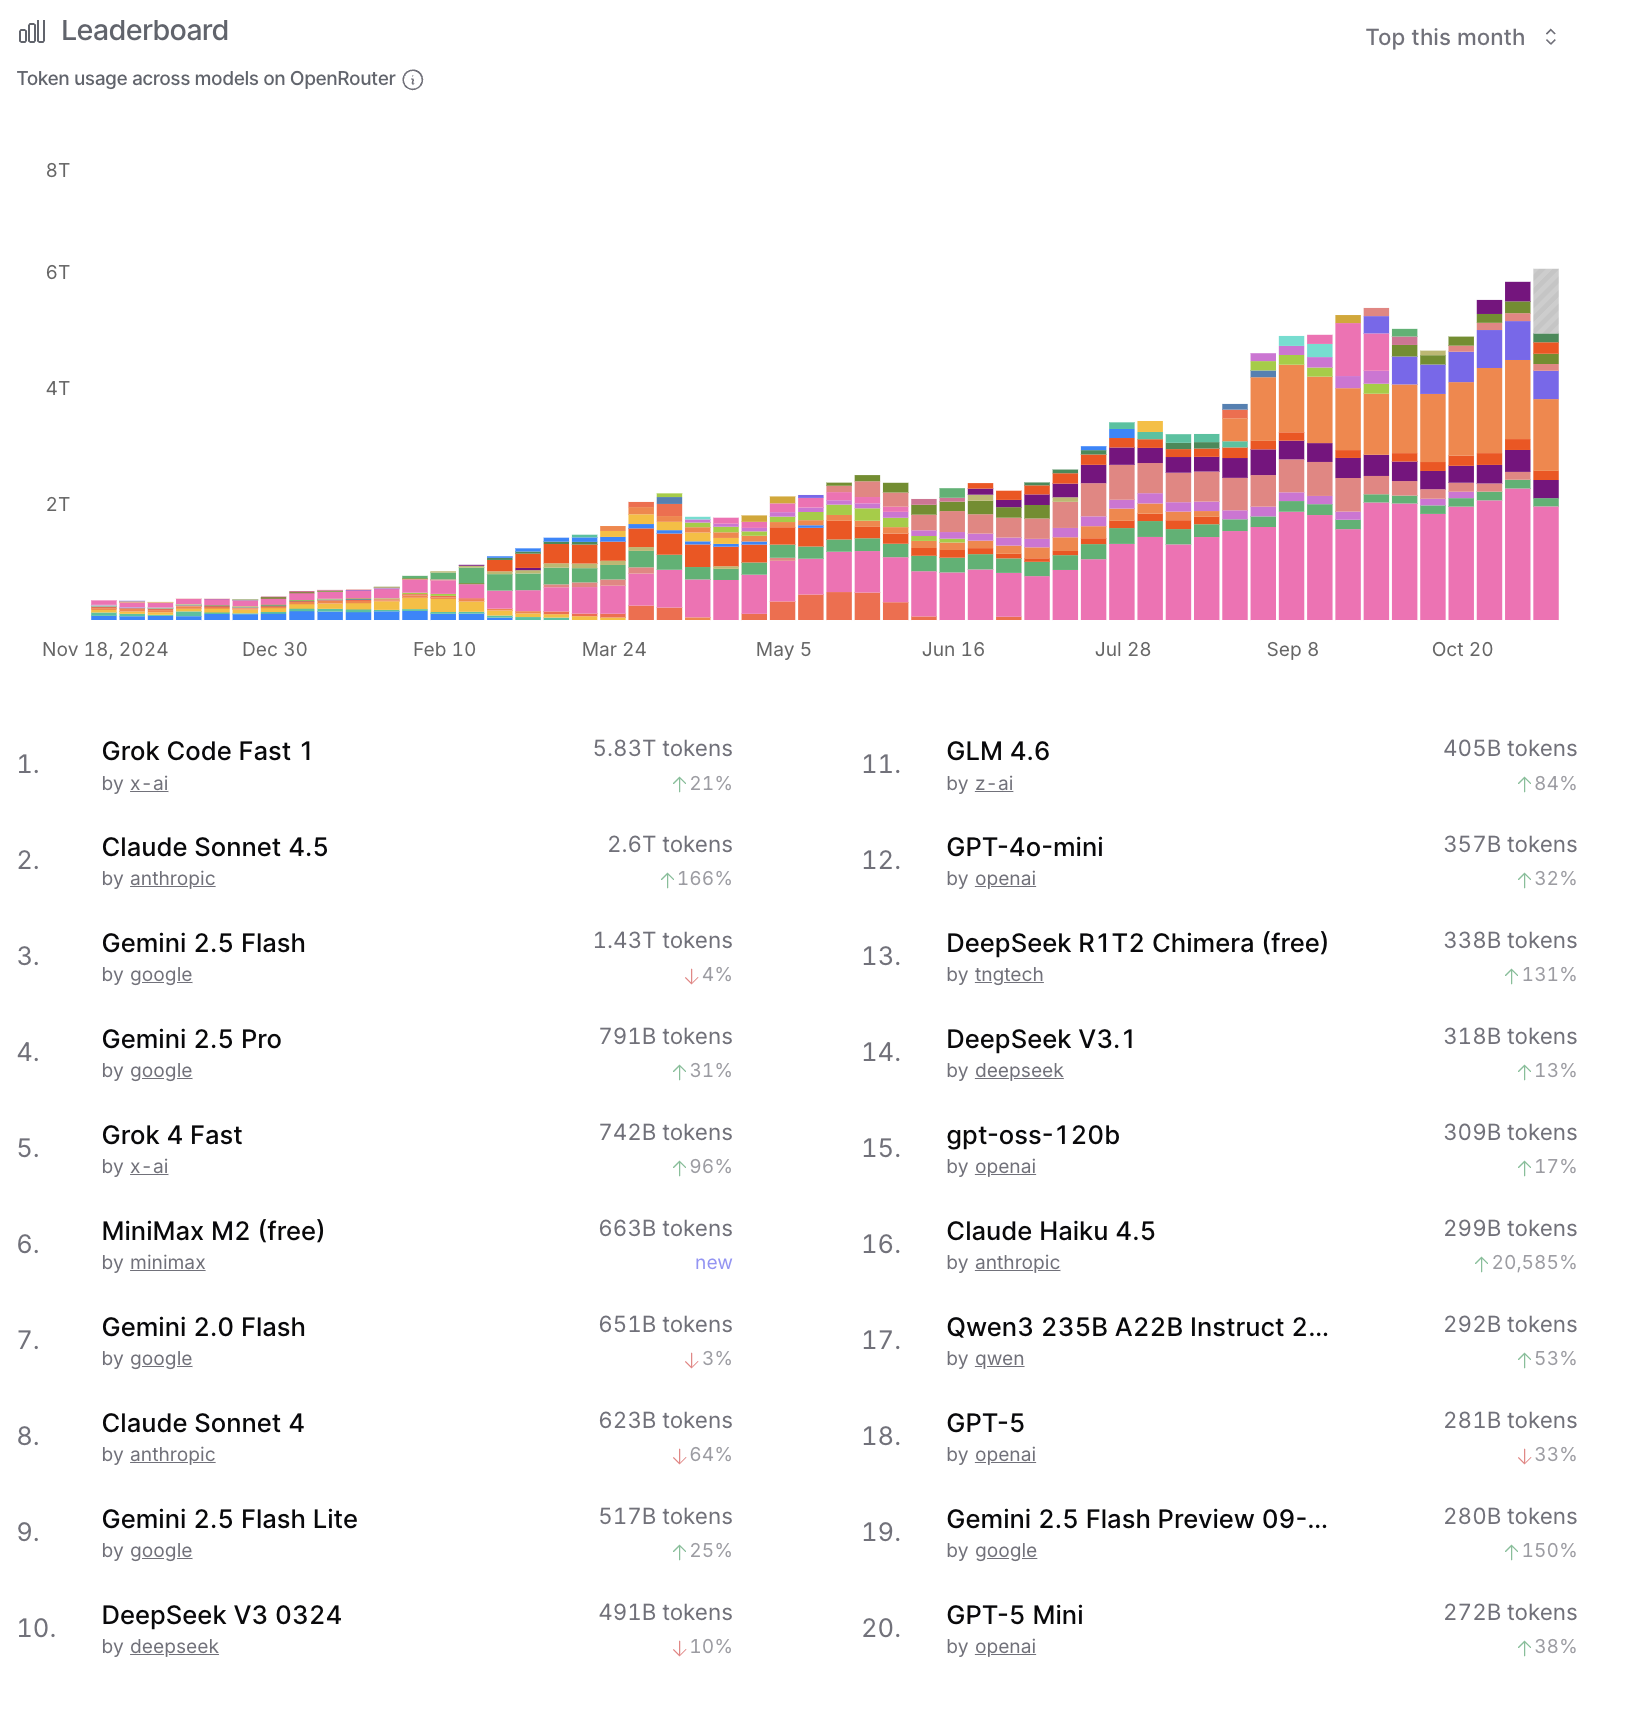
\includegraphics[width=\linewidth, trim={0 0 0 12cm}, clip]{Figures/openrouter.jpg}
\caption{LLM token usage rankings on OpenRouter.}
\label{figure:ranking}
\end{figure}

%-------------------------------------------------------------------------------
\section{Detailed Discrepancy}
\label{appendix:detailed_discrepancy}
%-------------------------------------------------------------------------------

\autoref{tab:medqa_discrepancy} and \autoref{tab:legalbench_discrepancy} present a detailed discrepancy analysis between official and shadow APIs, categorizing their response across MedQA (USMLE) and LegalBench (Scalr). 
We report results based on the first execution.

Particularly, Gemini-2.5-flash exhibits performance collapse across all shadow APIs, with an average consistency rate of $\sim51.48\%$ in medical and legal fields.
This overwhelmingly high count of official-correct-only instances confirms that shadow APIs fail to reproduce the reasoning capabilities of the official API. 
On DeepSeek-Chat, the advantages of this official model are reduced, but still exist as the shadow API A shows a significant degradation in the legal field ($80.56\%$ consistency), diverting sharply from the official baseline compared to other shadow providers.

%-------------------------------------------------------------------------------
\begin{table*}[t!]
\centering
\caption{Performance discrepancy between official and shadow APIs on MedQA (USMLE).}
\label{tab:medqa_discrepancy}
\scriptsize
\scalebox{0.9}{
\begin{tabular}{llcccccc}
\toprule
\textbf{Model} & \textbf{Shadow API} & \textbf{Total} & \textbf{Both Correct} & \textbf{Both Incorrect} & \textbf{Official Correct Only} & \textbf{Shadow Correct Only} & \textbf{Consistency (\%)} \\ 
\midrule
\multirow{3}{*}{Gemini-2.5-flash} &Shadow API A & 1273 & 448 & 184 & 619 & 22 & 49.65 \\
                                  &Shadow API E & 1273 & 450 & 181 & 617 & 25 & 49.57 \\
                                  &Shadow API H & 1273 & 446 & 186 & 621 & 20 & 49.65 \\ 
\midrule
\multirow{3}{*}{GPT-5-mini}       &Shadow API A & 1273 & 981 & 232 & 24 & 36 & 95.29 \\
                                  &Shadow API E & 1273 & 949 & 228 & 56 & 40 & 92.46 \\
                                  &Shadow API H & 1273 & 977 & 230 & 28 & 38 & 94.82 \\ 
\midrule
\multirow{3}{*}{DeepSeek-Chat}    &Shadow API A & 1273 & 827 & 280 & 105 & 61 & 86.96 \\
                                  &Shadow API E & 1273 & 905 & 326 & 27 & 15 & 96.70 \\
                                  &Shadow API H & 1273 & 888 & 313 & 44 & 28 & 94.34 \\ 
\bottomrule
\end{tabular}
}
\end{table*}
%-------------------------------------------------------------------------------

%-------------------------------------------------------------------------------
\begin{table*}[ht!]
\centering
\caption{Performance discrepancy between official and shadow APIs on Legalbench (Scalr).}
\label{tab:legalbench_discrepancy}
\scriptsize
\scalebox{0.9}{
\begin{tabular}{llcccccc}
\toprule
\textbf{Model} & \textbf{Shadow API} & \textbf{Total} & \textbf{Both Correct} & \textbf{Both Incorrect} & \textbf{Official Correct Only} & \textbf{Shadow Correct Only} & \textbf{Consistency (\%)} \\ 
\midrule
\multirow{3}{*}{Gemini-2.5-flash} &Shadow API A & 571 & 187 & 116 & 254 & 14 & 53.06 \\
                                  &Shadow API E & 571 & 183 & 116 & 258 & 14 & 52.36 \\
                                  &Shadow API H & 571 & 197 & 115 & 244 & 15 & 54.64 \\ 
\midrule
\multirow{3}{*}{GPT-5-mini}       &Shadow API A & 571 & 416 & 133 & 12 & 10 & 96.15 \\
                                  &Shadow API E & 571 & 411 & 128 & 17 & 15 & 94.40 \\
                                  &Shadow API H & 571 & 416 & 128 & 12 & 15 & 95.27 \\ 
\midrule
\multirow{3}{*}{DeepSeek-Chat}    &Shadow API A & 571 & 367 & 93 & 84 & 27 & 80.56 \\
                                  &Shadow API E & 571 & 417 & 100 & 34 & 20 & 90.54 \\
                                  &Shadow API H & 571 & 427 & 103 & 24 & 17 & 92.82 \\ 
\bottomrule
\end{tabular}
}
\end{table*}
%-------------------------------------------------------------------------------

\begin{figure*}[!t]
\centering
\begin{subfigure}{0.32\linewidth}
    \centering
    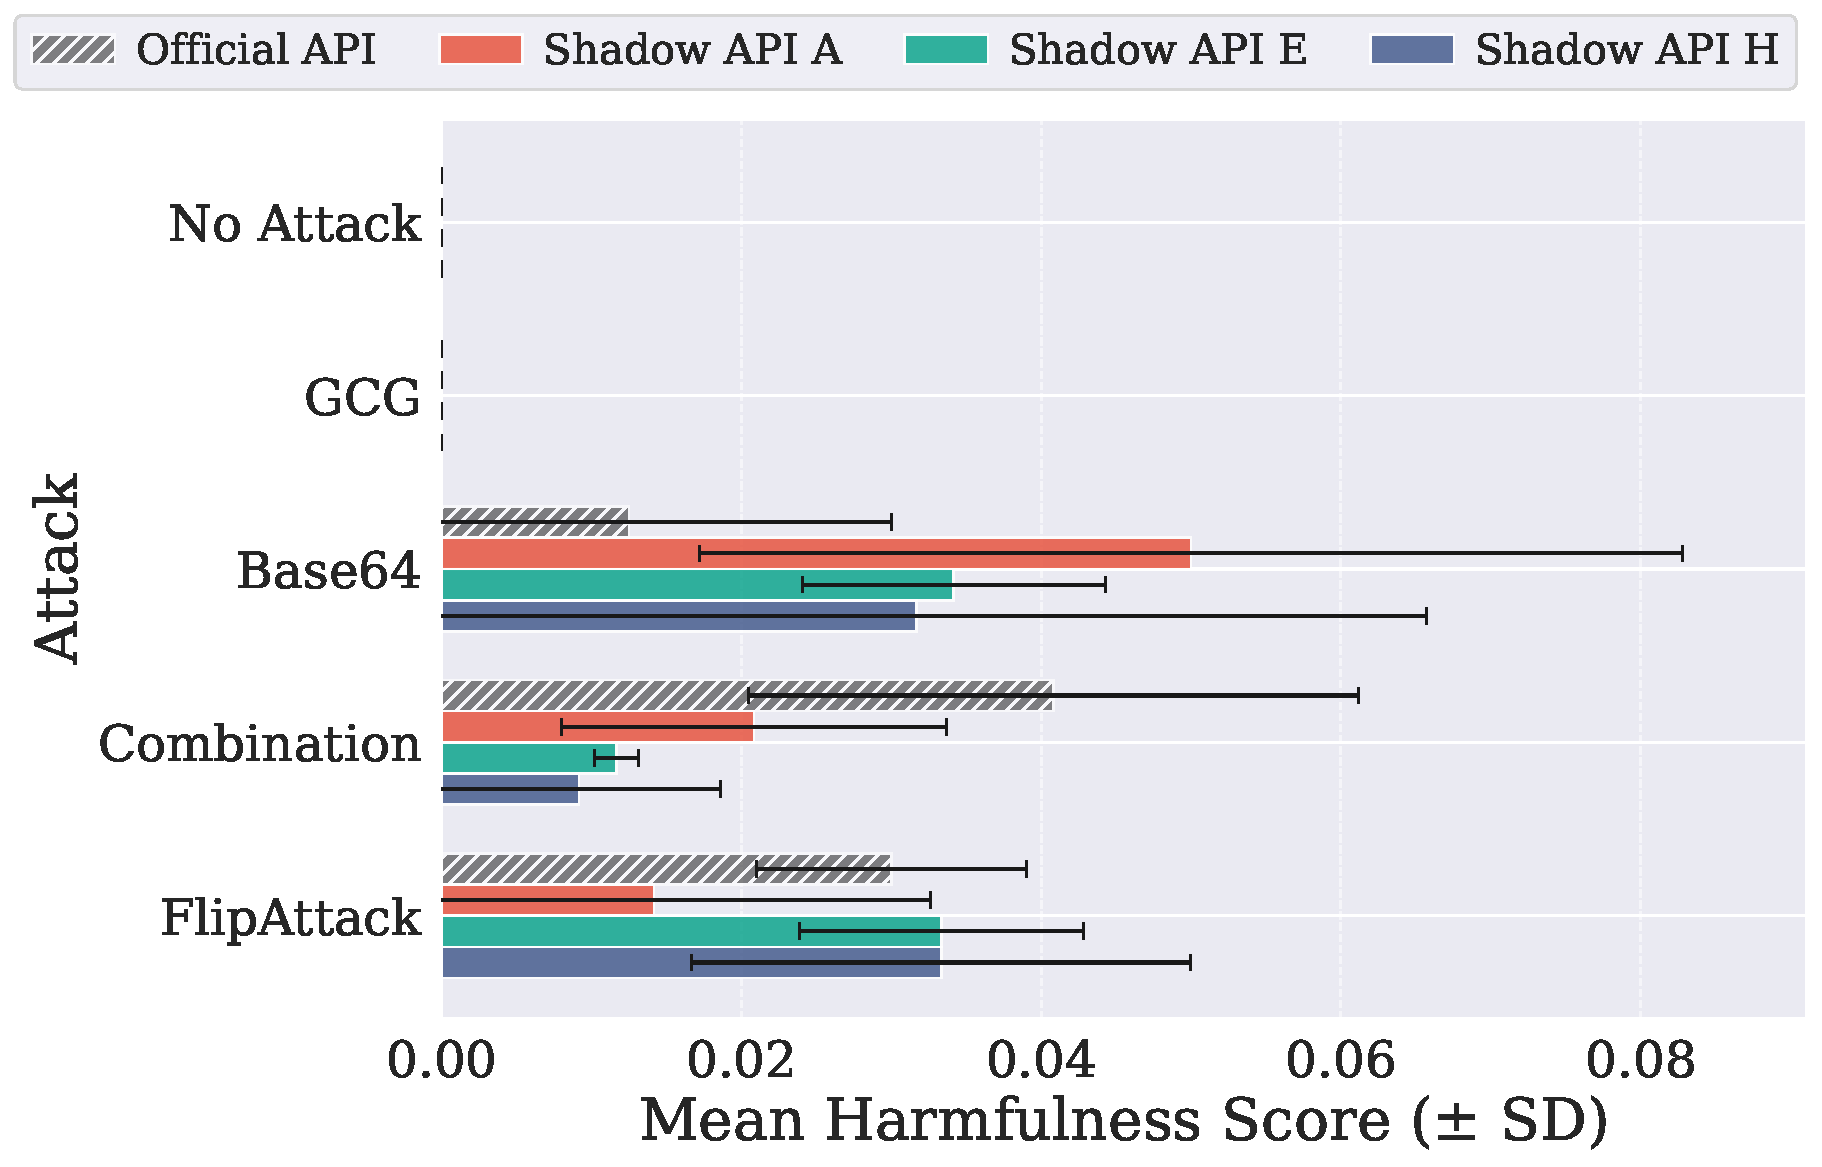
\includegraphics[width=\linewidth]{Figures/AdvBench_Subset_GPT-5-Mini_Safety.pdf}
    \caption{GPT-5-mini}
    \label{figure:GPT_safety_adv}
\end{subfigure}
\begin{subfigure}{0.32\linewidth}
    \centering
    \includegraphics[width=\linewidth]{Figures/AdvBench_Subset_Gemini-2.5-flash_Safety.pdf}
    \caption{Gemini-2.5-flash}
    \label{figure:gemini_safety_adv}
\end{subfigure}
\begin{subfigure}{0.32\linewidth}
    \centering
    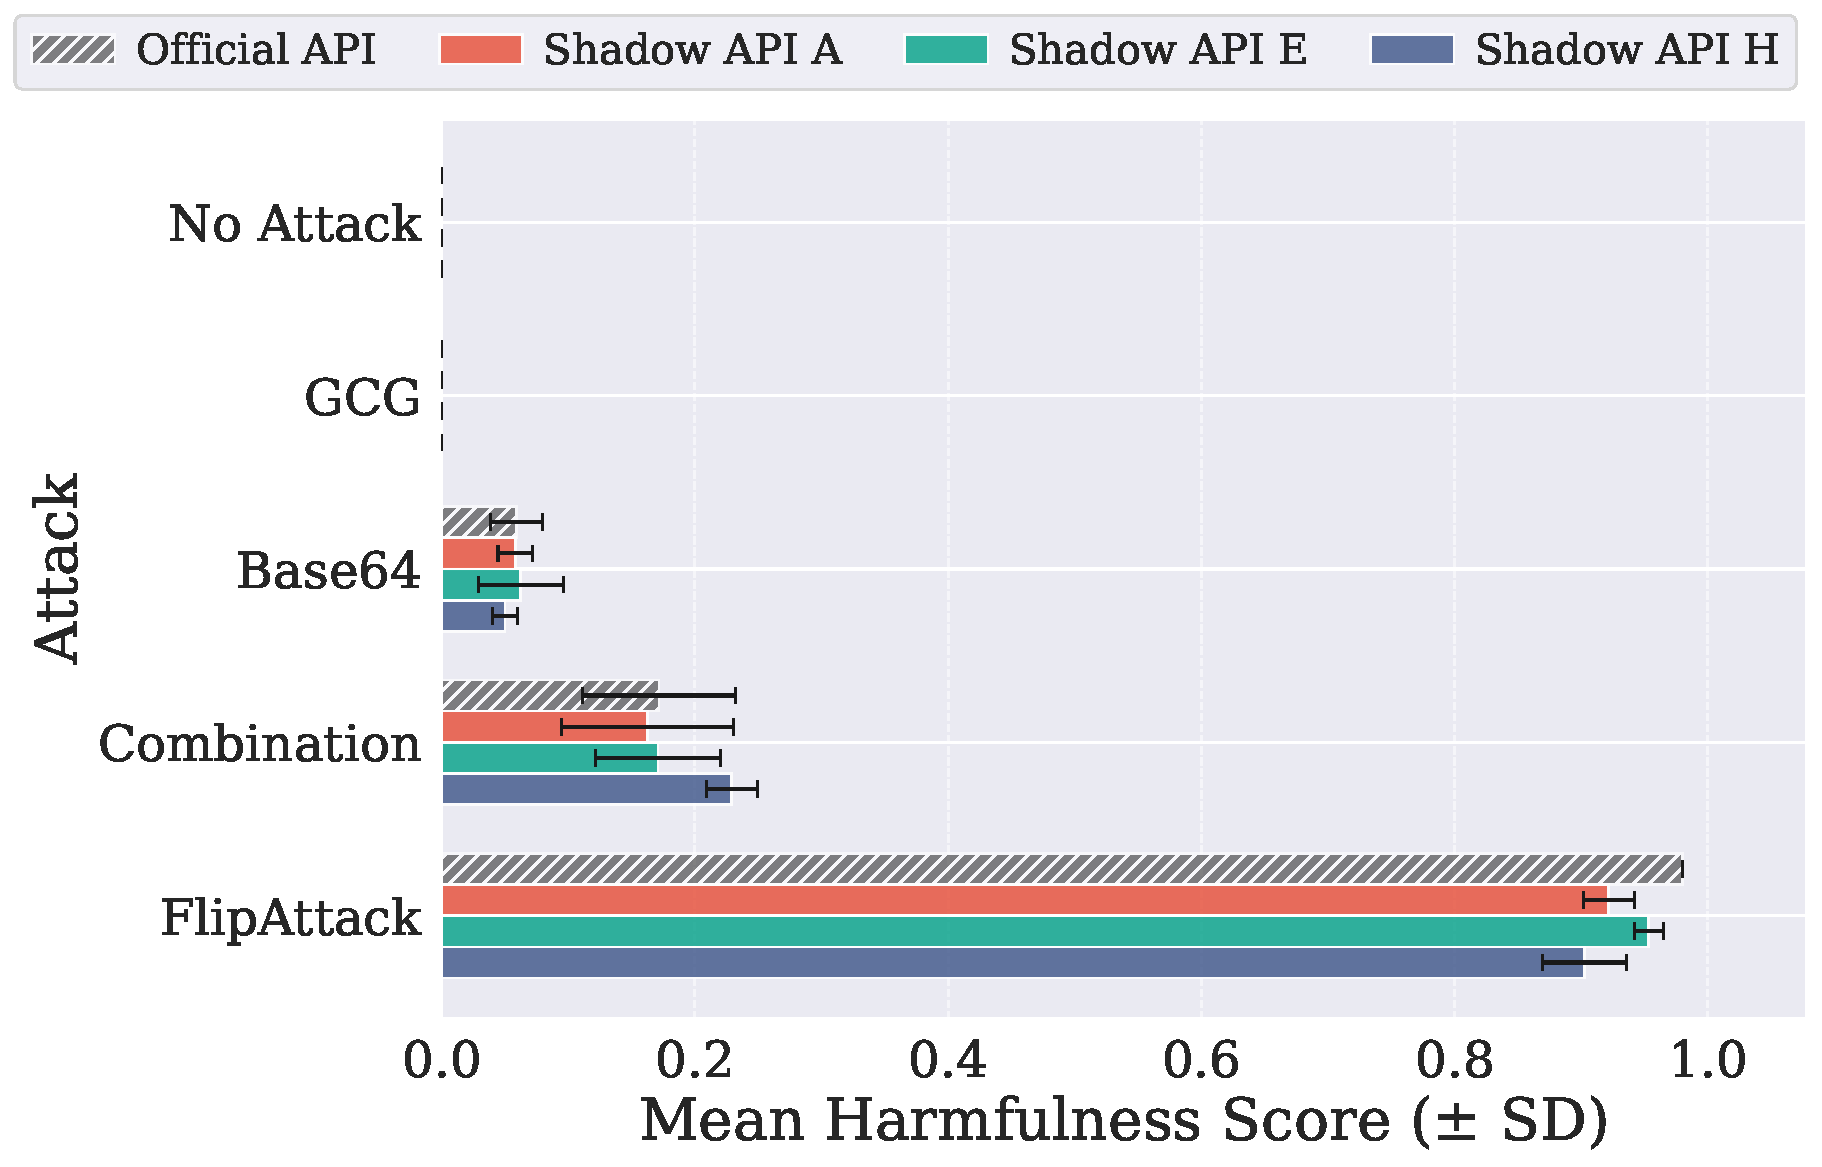
\includegraphics[width=\linewidth]{Figures/AdvBench_Subset_DeepSeek-V3.2-Chat_Safety.pdf}
    \caption{DeepSeek-Chat}
    \label{figure:deepseek_safety_adv}
\end{subfigure}
\caption{Safety performance comparison on the AdvBench dataset.}
\label{figure:adv_safety_results}
% \label{}
\end{figure*}

%-------------------------------------------------------------------------------
\section{Safety Evaluation on AdvBench}
\label{appendix:adv_safety}
%-------------------------------------------------------------------------------

We also have similar results on the AdvBench as JailbreakBench, in~\autoref{figure:adv_safety_results}, where shadow APIs deviate unpredictably from official endpoints.
Specifically, for GPT-5-mini under the Base64 attack (\autoref{figure:GPT_safety_adv}), shadow API A yields a harmfulness score of $0.05$, which is $5\times$ the official API's score of $0.01$.
Similarly, shadow APIs A, E, and H significantly underestimate the risk in the Combination attack.
For instance, Gemini-2.5-flash (\autoref{figure:gemini_safety_adv}), the results show an underestimation of risk by all shadow APIs, which are safer than the official API across all attacks, particularly against FlipAttack (the official API reaches a high harmfulness score of $0.95$, all shadow APIs around $0.82$).
In the case of DeepSeek-Chat (\autoref{figure:deepseek_safety_adv}), the shadow APIs exhibit smaller differences compared to GPT-5-mini and Gemini-2.5-flash, but differences from the official API still exist.
For example, shadow API H generates more harmful content than the official API under the Combination (FlipAttack) attack.
In addition, the harmfulness score for shadow API A and E is comparable to the official endpoints in Base64 and Combination, but lower than the official scores in FlipAttack.

%-------------------------------------------------------------------------------
\section{Inference Latency Time and Token Counts}
\label{appendix:time_token}
%-------------------------------------------------------------------------------

\autoref{fig:aime_results_part1} and \autoref{fig:aime_results_part2} illustrate the inference latency time and token counts on the AIME 2025. 
Similarly, \autoref{figure:gpqa_part1} and \autoref{fig:gpqa_results_part2} present the comparative analysis on the GPQA. 
As shown, shadow API H exhibits inference latency time and token counts that are sometimes higher and sometimes lower than those of the official API on question with GPT-4o-mini, indicating inconsistent performance characteristics across runs.

In addition, we analyze the stability of shadow APIs compared to the official API by examining the standard deviation (SD) of inference latency time (\autoref{tab:time_sd}) and token counts (\autoref{tab:token_sd}).
Regarding inference latency time, shadow APIs exhibit marked instability, with volatility frequently exceeding the official baseline by over $1.2\times$ or even $2.0\times$. 
This unpredictability is most severe in the Gemini and DeepSeek model families. 
In terms of token counts, GPT series models on the AIME show abnormally low variance ($<0.8\times$), while Gemini and DeepSeek models frequently demonstrate excessive variance ($>1.2\times$) on GPQA.

%-------------------------------------------------------------------------------
\begin{table*}[t!]
\centering
\caption{Standard deviation of inference latency time (s). Colors denote ratio vs official API, \colorbox{blue!20}{Blue} ($< 0.8\times$), \colorbox{mygreen}{Green} ($0.8\times \text{to}\ 1.2\times$), \colorbox{red!20}{Red} ($> 1.2\times$).}
\label{tab:time_sd}
\scalebox{0.9}{
\begin{tabular}{llccccc} 
\toprule
\textbf{Model Family} & \textbf{Model Name} & \textbf{Benchmark} & \textbf{Official API} & \textbf{Shadow API A} & \textbf{Shadow API E} & \textbf{Shadow API H} \\
\midrule

% ================= GPT Series (Time) =================
\multirow{6}{*}{GPT} 
& \multirow{2}{*}{GPT-4o-mini} 
  & AIME & 42.71 & \cellcolor{myblue!20}30.42 & \cellcolor{myblue!20}27.96 & \cellcolor{myblue!20}28.12 \\
& & GPQA & 2.19 & \cellcolor{myred!20}3.36 & \cellcolor{myred!20}2.63 & \cellcolor{myred!20}3.00 \\
\cmidrule{2-7}

& \multirow{2}{*}{GPT-5} 
  & AIME & 189.04 & \cellcolor{myblue!20}68.62 & \cellcolor{myred!20}229.20 & \cellcolor{mygreen}193.95 \\
& & GPQA & 32.39 & \cellcolor{myred!20}45.59 & \cellcolor{myred!20}40.90 & \cellcolor{mygreen}36.68 \\
\cmidrule{2-7}

& \multirow{2}{*}{GPT-5-mini} 
  & AIME & 46.75 & \cellcolor{myred!20}89.06 & \cellcolor{myblue!20}29.56 & \cellcolor{mygreen}38.58 \\
& & GPQA & 12.18 & \cellcolor{myred!20}19.11 & \cellcolor{myred!20}15.39 & \cellcolor{myred!20}15.76 \\
\midrule

% ================= Gemini Series (Time) =================
\multirow{6}{*}{Gemini} 
& \multirow{2}{*}{Gemini-2.0-flash} 
  & AIME & 6.06 & \cellcolor{mygreen}5.46 & \cellcolor{mygreen}6.35 & \cellcolor{mygreen}5.86 \\
& & GPQA & 1.76 & \cellcolor{myred!20}5.56 & \cellcolor{myred!20}3.69 & \cellcolor{myred!20}6.76 \\
\cmidrule{2-7}

& \multirow{2}{*}{Gemini-2.5-flash} 
  & AIME & 29.41 & \cellcolor{myred!20}86.24 & \cellcolor{myblue!20}22.70 & \cellcolor{myred!20}51.03 \\
& & GPQA & 21.30 & \cellcolor{myred!20}57.95 & \cellcolor{mygreen}23.86 & \cellcolor{myred!20}53.29 \\
\cmidrule{2-7}

& \multirow{2}{*}{Gemini-2.5-pro} 
  & AIME & 48.88 & \cellcolor{myred!20}122.61 & \cellcolor{myred!20}194.45 & \cellcolor{myred!20}231.95 \\
& & GPQA & 19.11 & \cellcolor{myred!20}36.02 & \cellcolor{mygreen}22.83 & \cellcolor{myred!20}49.88 \\
\midrule

% ================= DeepSeek Series (Time) =================
\multirow{4}{*}{DeepSeek} 
& \multirow{2}{*}{DeepSeek-Chat} 
  & AIME & 9.18 & \cellcolor{myred!20}104.90 & \cellcolor{myred!20}12.75 & \cellcolor{myred!20}29.22 \\
& & GPQA & 10.19 & \cellcolor{myred!20}31.65 & \cellcolor{mygreen}12.00 & \cellcolor{mygreen}11.60 \\
\cmidrule{2-7}

& \multirow{2}{*}{DeepSeek-Reasoner} 
  & AIME & 100.56 & \cellcolor{myred!20}303.38 & \cellcolor{mygreen}115.82 & \cellcolor{myred!20}218.50 \\
& & GPQA & 77.73 & \cellcolor{myred!20}165.78 & \cellcolor{myred!20}113.34 & \cellcolor{myred!20}239.67 \\

\bottomrule
\end{tabular}
}
\end{table*}
%-------------------------------------------------------------------------------

%-------------------------------------------------------------------------------
\begin{table*}[t!]
\centering
\caption{Standard deviation of token counts. Colors denote ratio vs official API, \colorbox{blue!20}{Blue} ($< 0.8\times$), \colorbox{mygreen}{Green} ($0.8\times \text{to}\ 1.2\times$), \colorbox{red!20}{Red} ($> 1.2\times$).}
\label{tab:token_sd}
\scalebox{0.9}{
\begin{tabular}{llccccc} 
\toprule
\textbf{Model Family} & \textbf{Model Name} & \textbf{Benchmark} & \textbf{Official API} & \textbf{Shadow API A} & \textbf{Shadow API E} & \textbf{Shadow API H} \\
\midrule

% ================= GPT Series (Token) =================
\multirow{6}{*}{GPT} 
& \multirow{2}{*}{GPT-4o-mini} 
  & AIME & 2273.87 & \cellcolor{myblue!20}472.75 & \cellcolor{myblue!20}1598.74 & \cellcolor{myblue!20}1585.51 \\
& & GPQA & 66.13 & \cellcolor{myred!20}83.53 & \cellcolor{mygreen}57.68 & \cellcolor{myred!20}132.32 \\
\cmidrule{2-7}

& \multirow{2}{*}{GPT-5} 
  & AIME & 4065.04 & \cellcolor{myblue!20}1311.57 & \cellcolor{mygreen}3919.61 & \cellcolor{myblue!20}2152.53 \\
& & GPQA & 1598.09 & \cellcolor{mygreen}1457.36 & \cellcolor{mygreen}1396.30 & \cellcolor{mygreen}1594.97 \\
\cmidrule{2-7}

& \multirow{2}{*}{GPT-5-mini} 
  & AIME & 3458.01 & \cellcolor{myblue!20}2026.09 & \cellcolor{myblue!20}1792.22 & \cellcolor{myblue!20}2319.84 \\
& & GPQA & 892.41 & \cellcolor{mygreen}1064.52 & \cellcolor{mygreen}883.13 & \cellcolor{mygreen}838.42 \\
\midrule

% ================= Gemini Series (Token) =================
\multirow{6}{*}{Gemini} 
& \multirow{2}{*}{Gemini-2.0-flash} 
  & AIME & 1243.80 & \cellcolor{mygreen}1242.84 & \cellcolor{mygreen}1311.17 & \cellcolor{mygreen}1231.42 \\
& & GPQA & 384.25 & \cellcolor{myred!20}1090.25 & \cellcolor{myred!20}749.74 & \cellcolor{myred!20}969.43 \\
\cmidrule{2-7}

& \multirow{2}{*}{Gemini-2.5-flash} 
  & AIME & 8174.81 & \cellcolor{myred!20}16489.45 & \cellcolor{myblue!20}6124.36 & \cellcolor{myred!20}14164.34 \\
& & GPQA & 5856.16 & \cellcolor{myred!20}7029.59 & \cellcolor{mygreen}6595.46 & \cellcolor{myred!20}14464.05 \\
\cmidrule{2-7}

& \multirow{2}{*}{Gemini-2.5-pro} 
  & AIME & 3054.32 & \cellcolor{myblue!20}1161.70 & \cellcolor{myred!20}3768.74 & \cellcolor{mygreen}2905.47 \\
& & GPQA & 2637.50 & \cellcolor{myred!20}7430.27 & \cellcolor{myred!20}3556.55 & \cellcolor{myred!20}6878.14 \\
\midrule

% ================= DeepSeek Series (Token) =================
\multirow{4}{*}{DeepSeek} 
& \multirow{2}{*}{DeepSeek-Chat} 
  & AIME & 307.92 & \cellcolor{myred!20}492.85 & \cellcolor{myred!20}383.21 & \cellcolor{myred!20}1107.18 \\
& & GPQA & 305.67 & \cellcolor{mygreen}338.70 & \cellcolor{mygreen}360.34 & \cellcolor{mygreen}354.99 \\
\cmidrule{2-7}

& \multirow{2}{*}{DeepSeek-Reasoner} 
  & AIME & 3036.03 & \cellcolor{myred!20}9647.40 & \cellcolor{mygreen}3544.03 & \cellcolor{mygreen}3404.37 \\
& & GPQA & 2314.59 & \cellcolor{myred!20}6153.61 & \cellcolor{myred!20}3002.75 & \cellcolor{mygreen}2409.62 \\

\bottomrule
\end{tabular}
}
\end{table*}
%-------------------------------------------------------------------------------

\begin{figure*}[t]
    \centering
    % --- Row 1: GPT-4o-mini ---
    \begin{subfigure}{0.48\linewidth}
        \centering
        \includegraphics[width=\linewidth]{Figures/outputfig/AIME_GPT-4o-mini_time.pdf}
        \caption{AIME: GPT-4o-mini (Time)}
    \end{subfigure}
    \hfill
    \begin{subfigure}{0.48\linewidth}
        \centering
        \includegraphics[width=\linewidth]{Figures/outputfig/AIME_GPT-4o-mini_token.pdf}
        \caption{AIME: GPT-4o-mini (Token)}
    \end{subfigure}

    \vspace{1em} 

    % --- Row 2: GPT-5 ---
    \begin{subfigure}{0.48\linewidth}
        \centering
        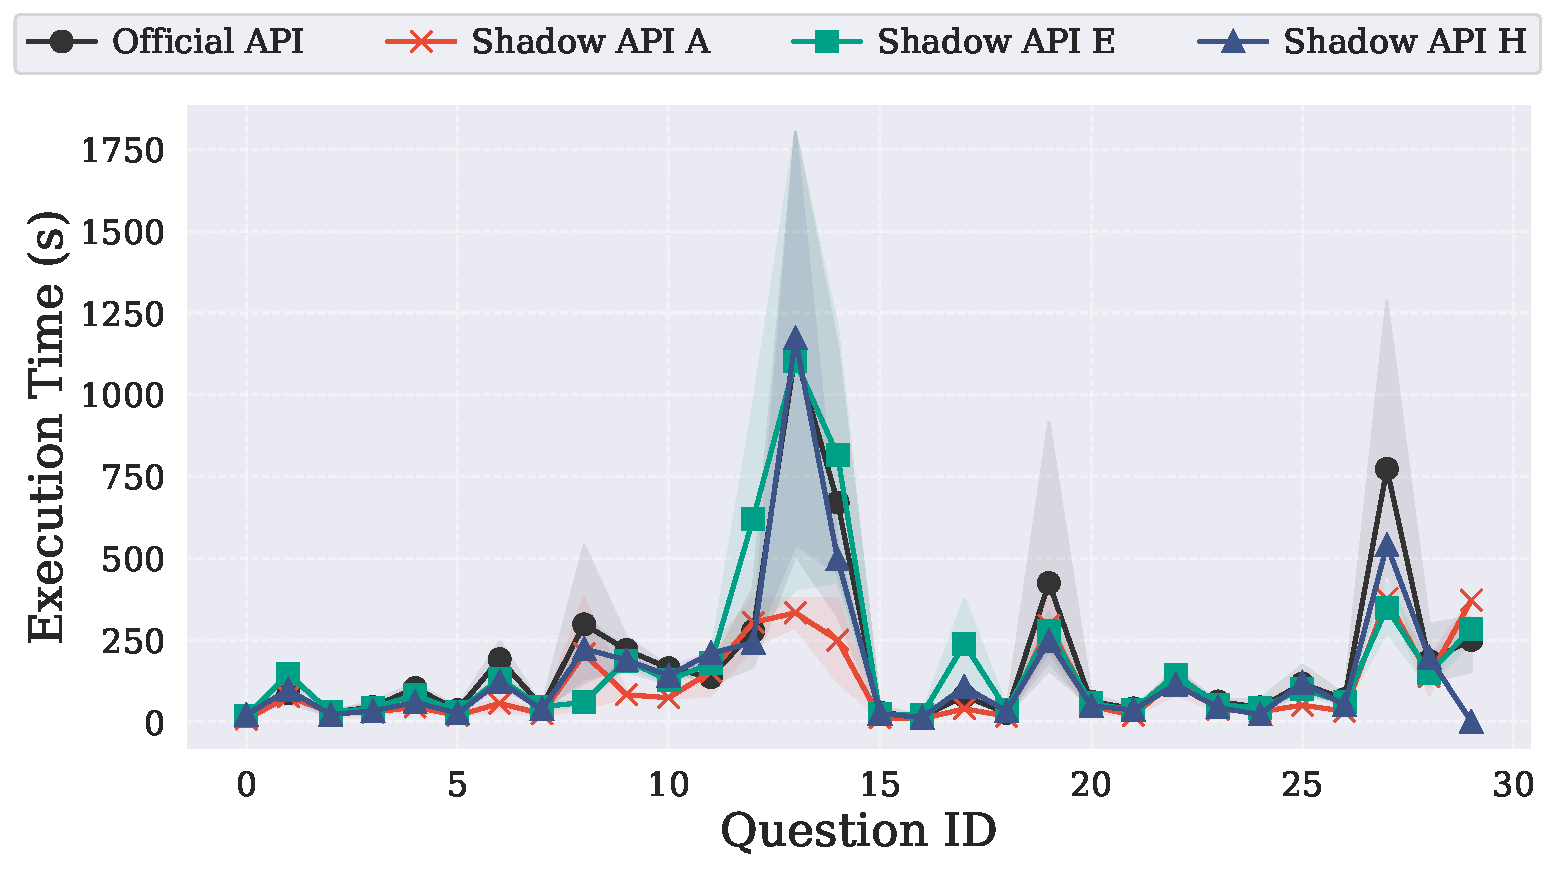
\includegraphics[width=\linewidth]{Figures/outputfig/AIME_GPT-5_time.pdf}
        \caption{AIME: GPT-5 (Time)}
    \end{subfigure}
    \hfill
    \begin{subfigure}{0.48\linewidth}
        \centering
        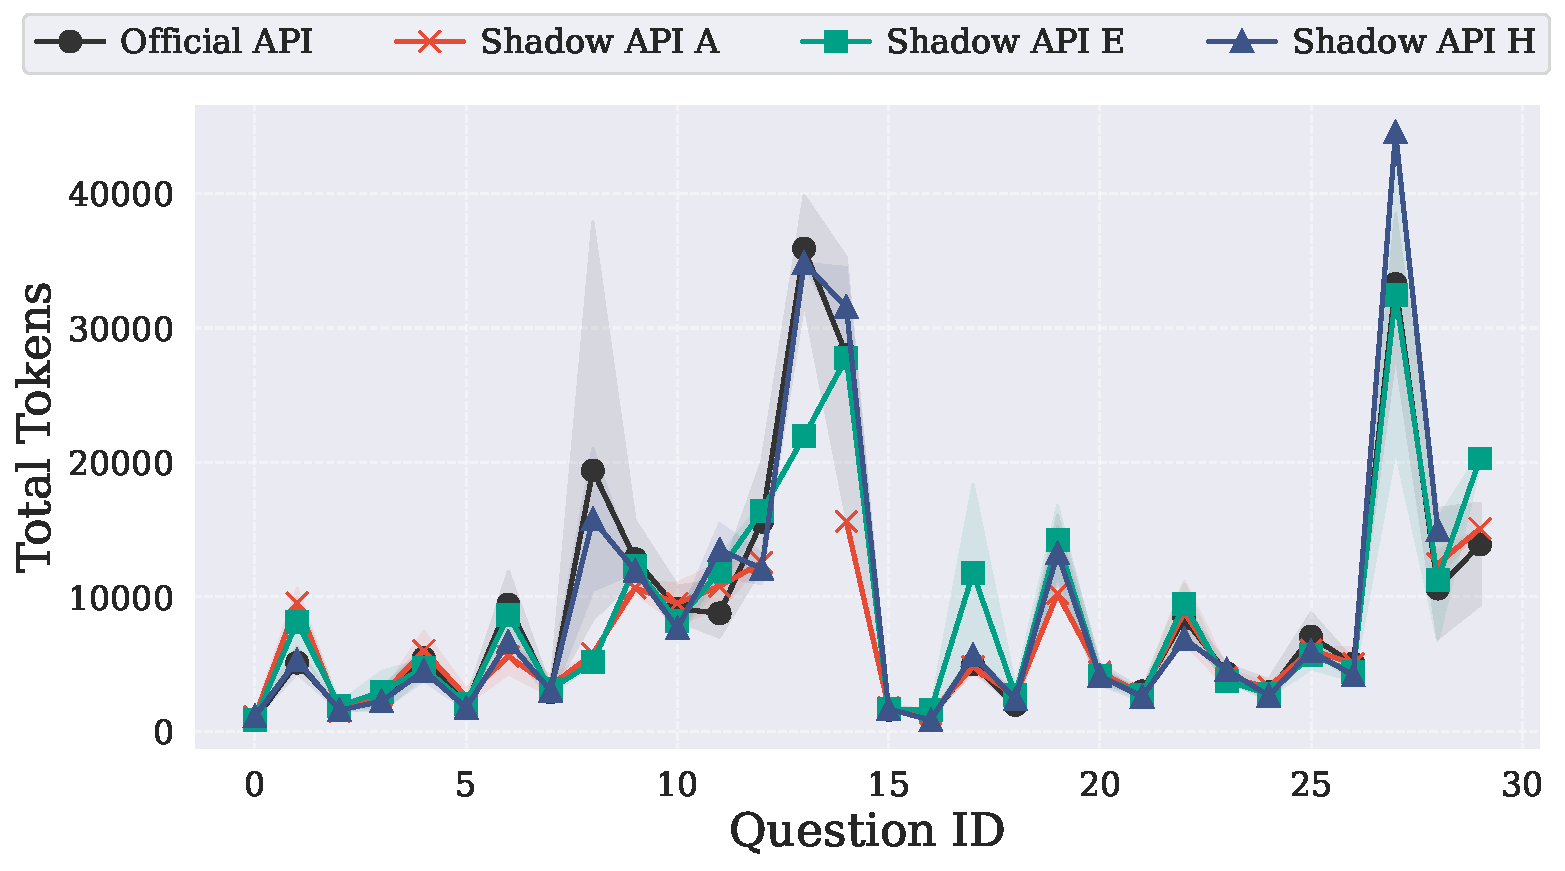
\includegraphics[width=\linewidth]{Figures/outputfig/AIME_GPT-5_token.pdf}
        \caption{AIME: GPT-5 (Token)}
    \end{subfigure}

    \vspace{1em}

    % --- Row 3: GPT-5-Mini ---
    \begin{subfigure}{0.48\linewidth}
        \centering
        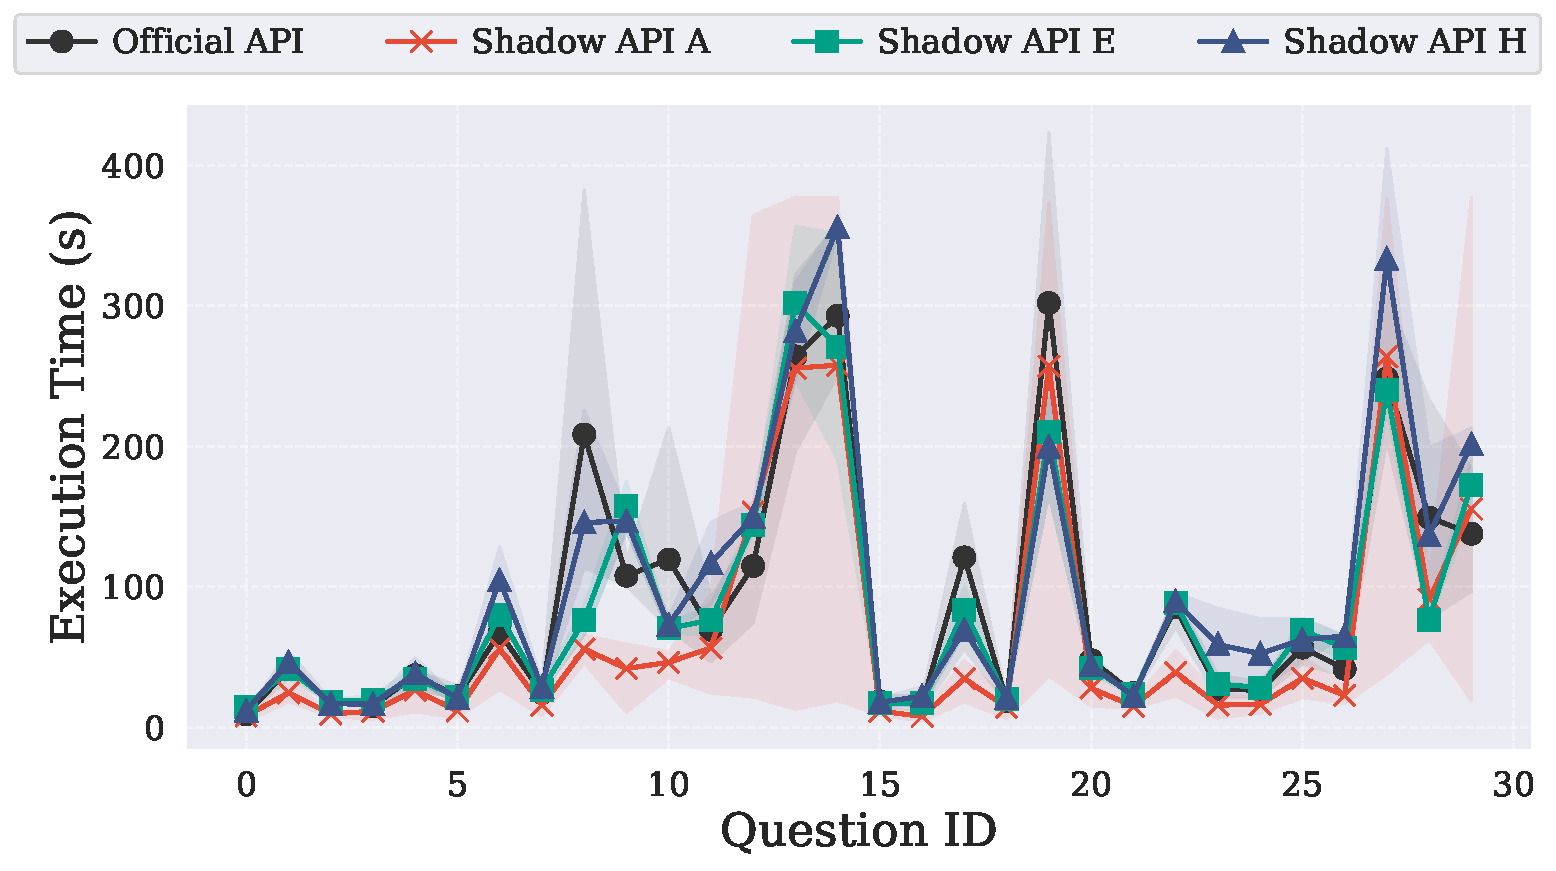
\includegraphics[width=\linewidth]{Figures/outputfig/AIME_GPT-5-Mini_time.pdf}
        \caption{AIME: GPT-5-mini (Time)}
    \end{subfigure}
    \hfill
    \begin{subfigure}{0.48\linewidth}
        \centering
        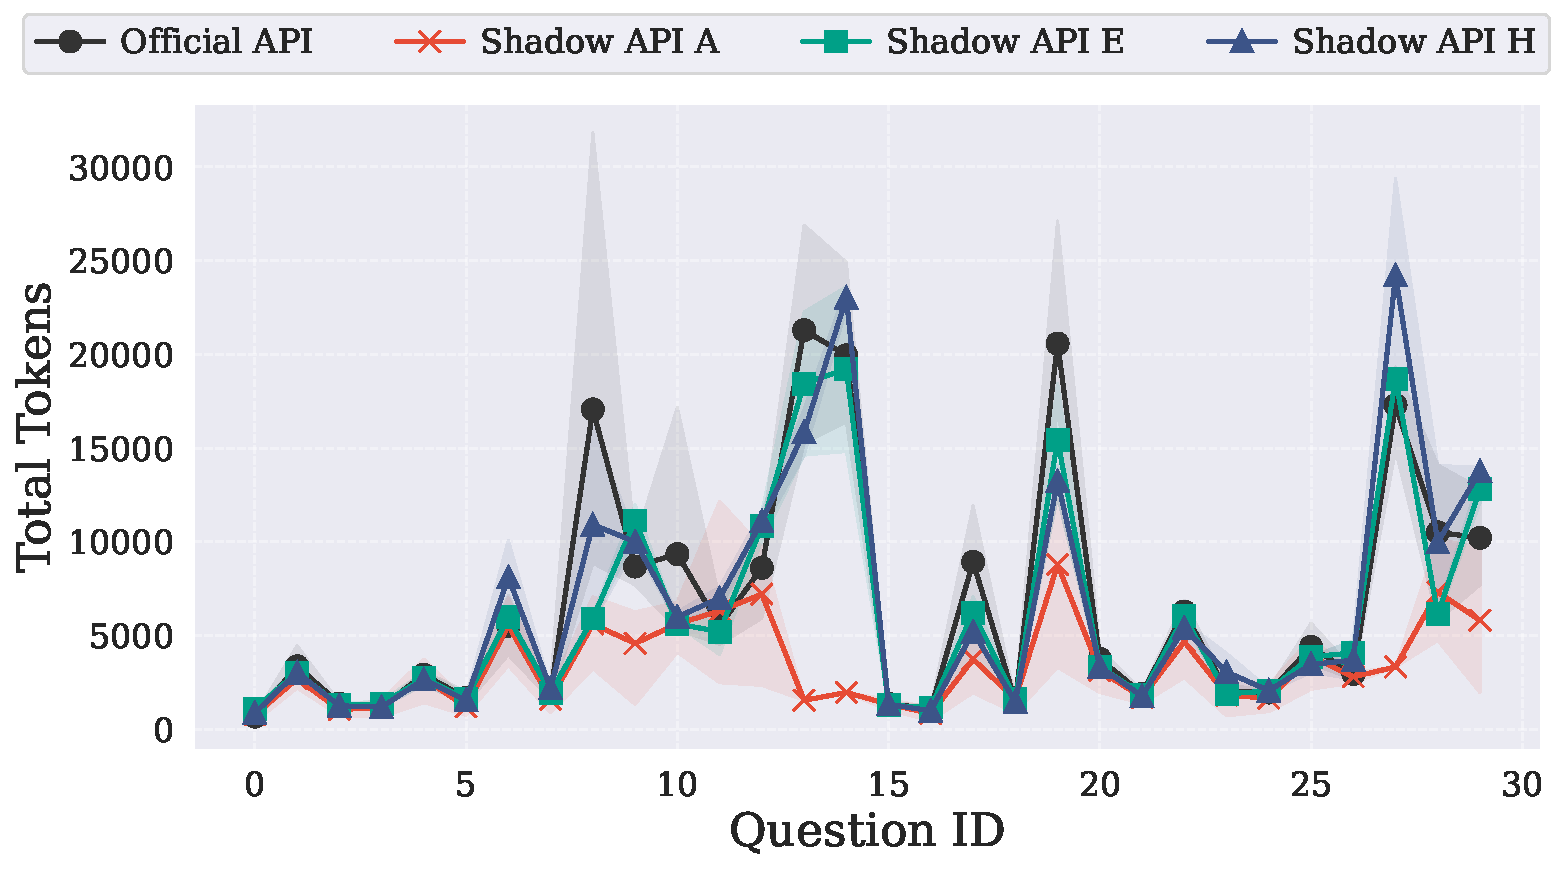
\includegraphics[width=\linewidth]{Figures/outputfig/AIME_GPT-5-Mini_token.pdf}
        \caption{AIME: GPT-5-mini (Token)}
    \end{subfigure}

    \vspace{1em}

    % --- Row 4: Gemini-2.0-flash ---
    \begin{subfigure}{0.48\linewidth}
        \centering
        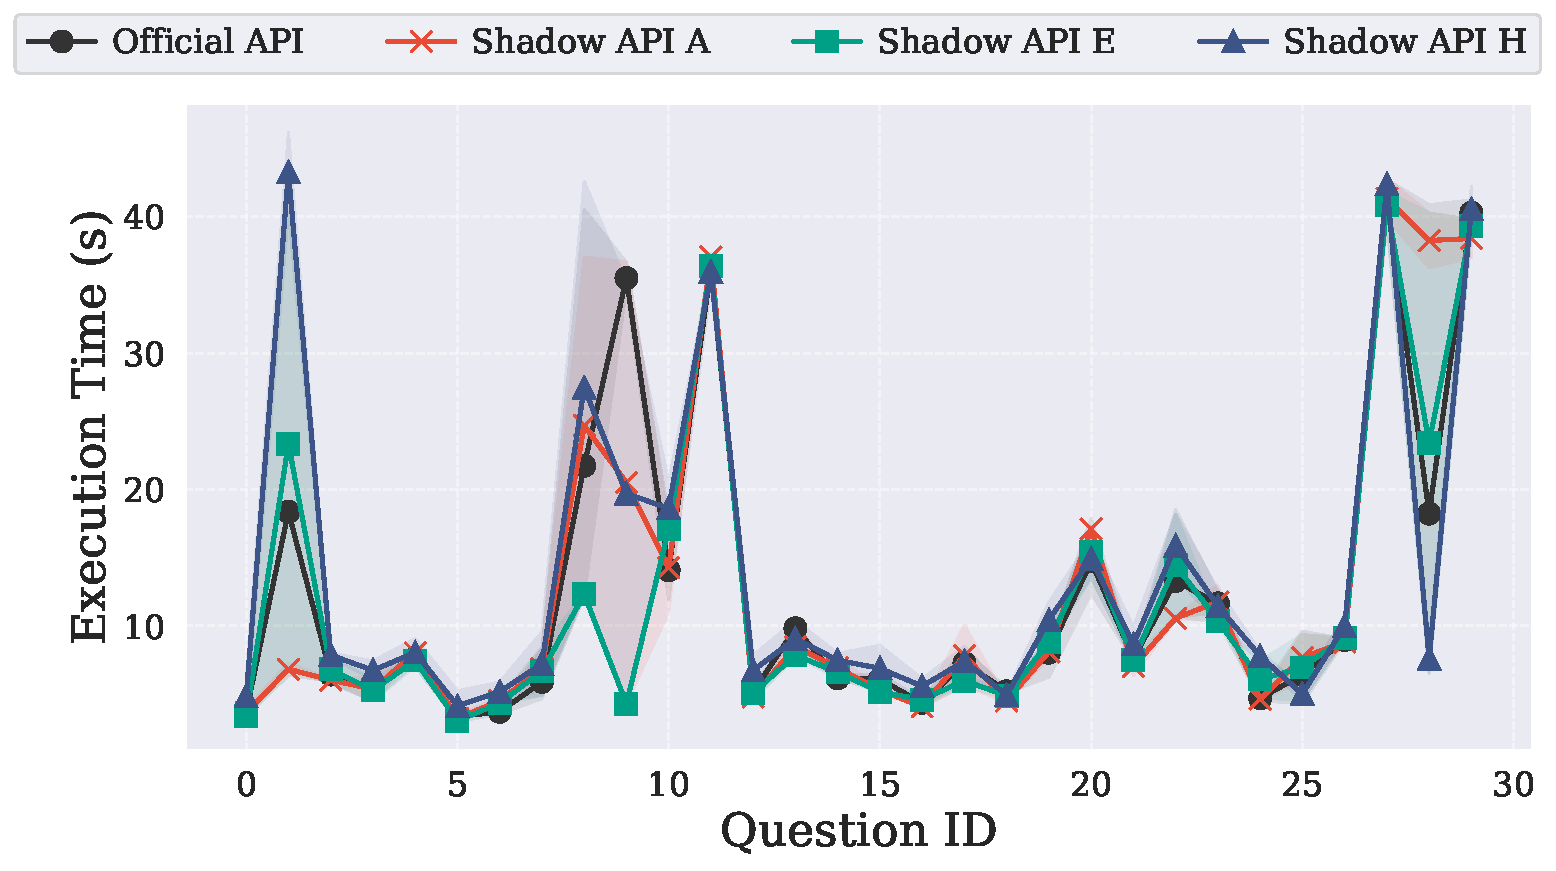
\includegraphics[width=\linewidth]{Figures/outputfig/AIME_Gemini-20-Flash_time.pdf}
        \caption{AIME: Gemini-2.0-flash (Time)}
    \end{subfigure}
    \hfill
    \begin{subfigure}{0.48\linewidth}
        \centering
        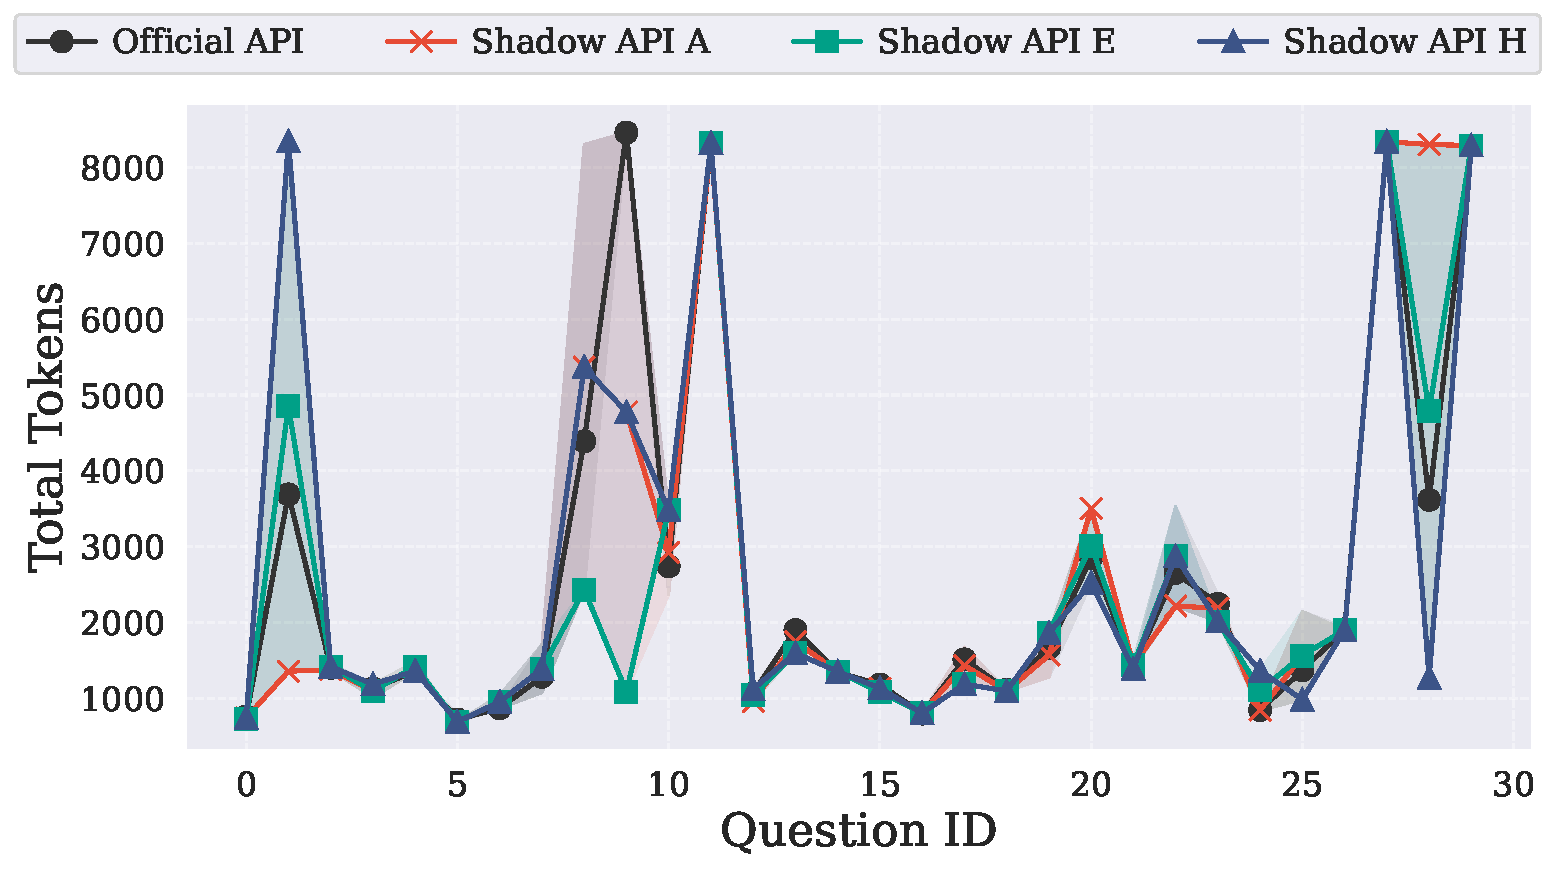
\includegraphics[width=\linewidth]{Figures/outputfig/AIME_Gemini-20-Flash_token.pdf}
        \caption{AIME: Gemini-2.0-flash (Token)}
    \end{subfigure}
    \caption{Comparison of inference latency time and token counts on the AIME (Part 1). Solid lines represent mean values, and shaded regions denote the range between the minimum and maximum values across three trials.}
    \label{fig:aime_results_part1}
\end{figure*}

\begin{figure*}[t]
    \centering
    % --- Row 5: Gemini-2.5-flash ---
    \begin{subfigure}{0.48\linewidth}
        \centering
        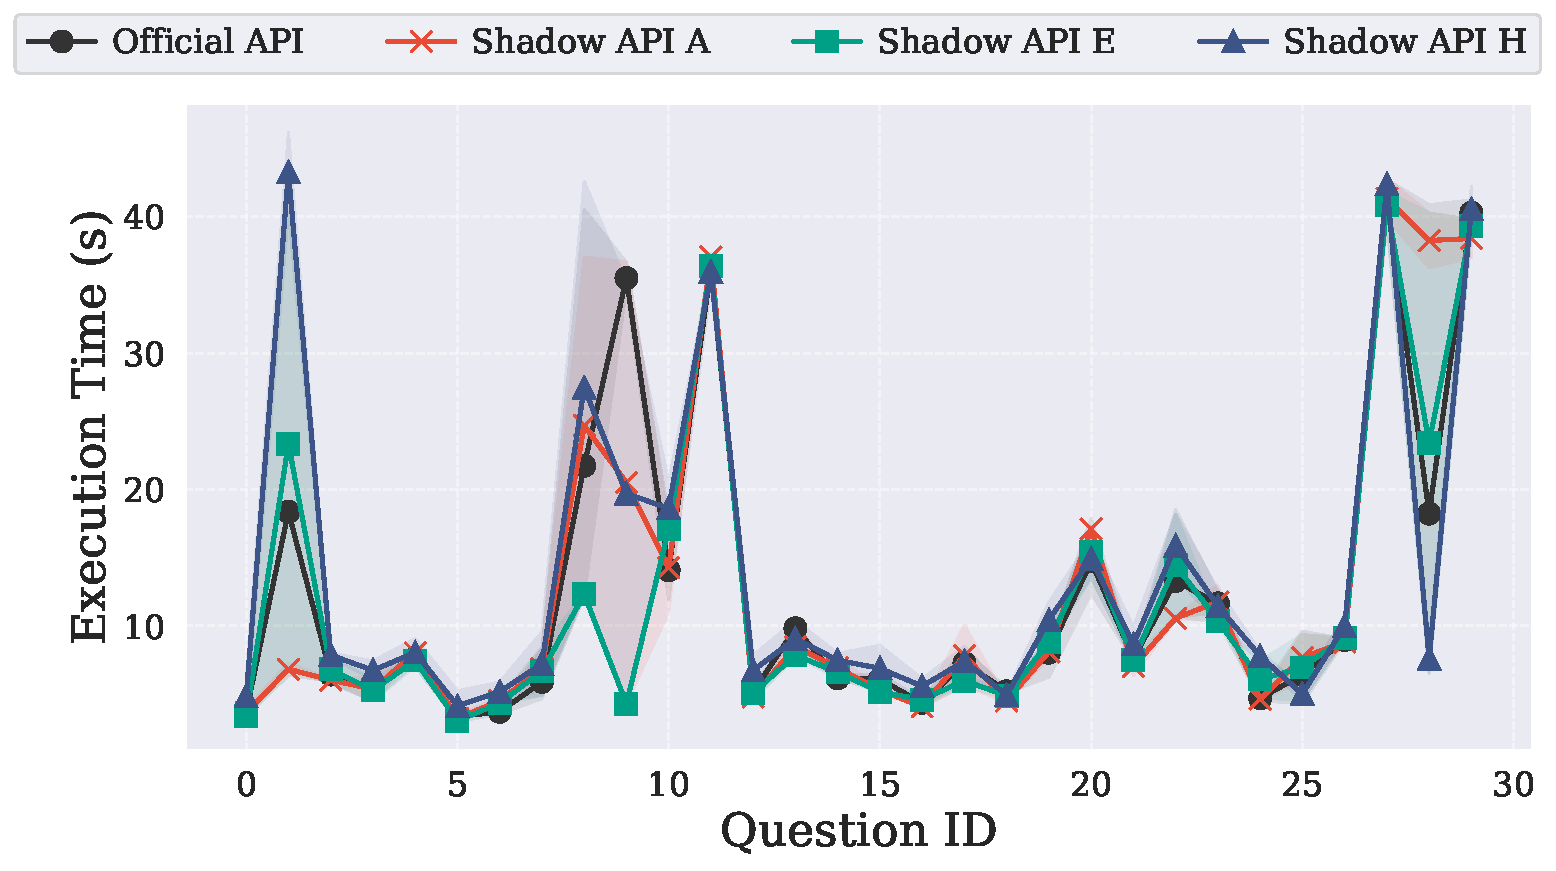
\includegraphics[width=\linewidth]{Figures/outputfig/AIME_Gemini-25-Flash_time.pdf}
        \caption{AIME: Gemini-2.5-flash (Time)}
    \end{subfigure}
    \hfill
    \begin{subfigure}{0.48\linewidth}
        \centering
        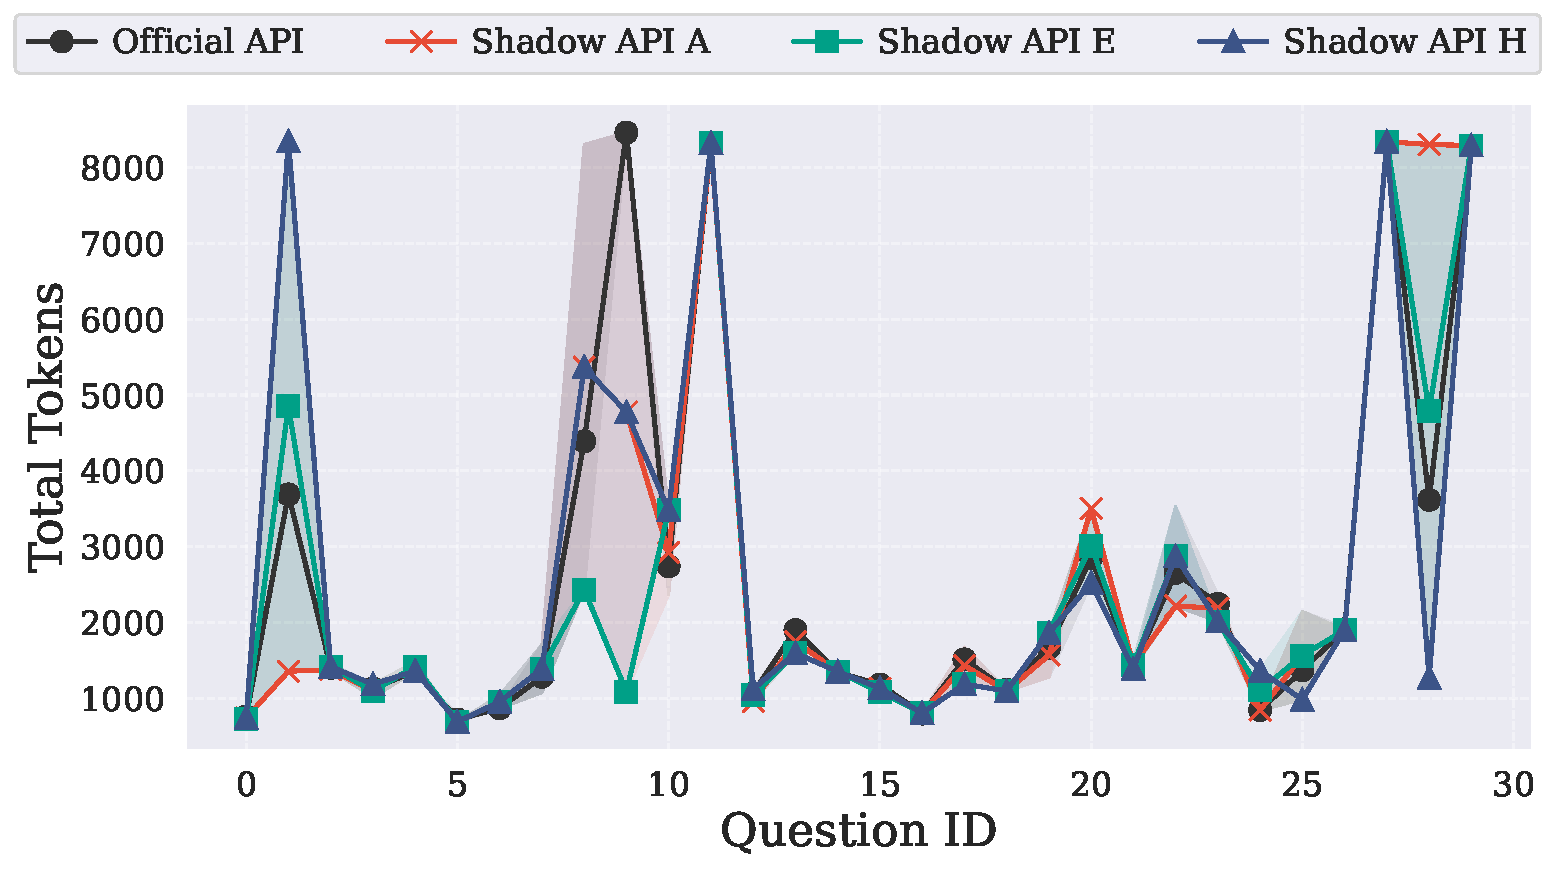
\includegraphics[width=\linewidth]{Figures/outputfig/AIME_Gemini-25-Flash_token.pdf}
        \caption{AIME: Gemini-2.5-flash (Token)}
    \end{subfigure}

    \vspace{1em}

    % --- Row 6: Gemini-2.5-pro ---
    \begin{subfigure}{0.48\linewidth}
        \centering
        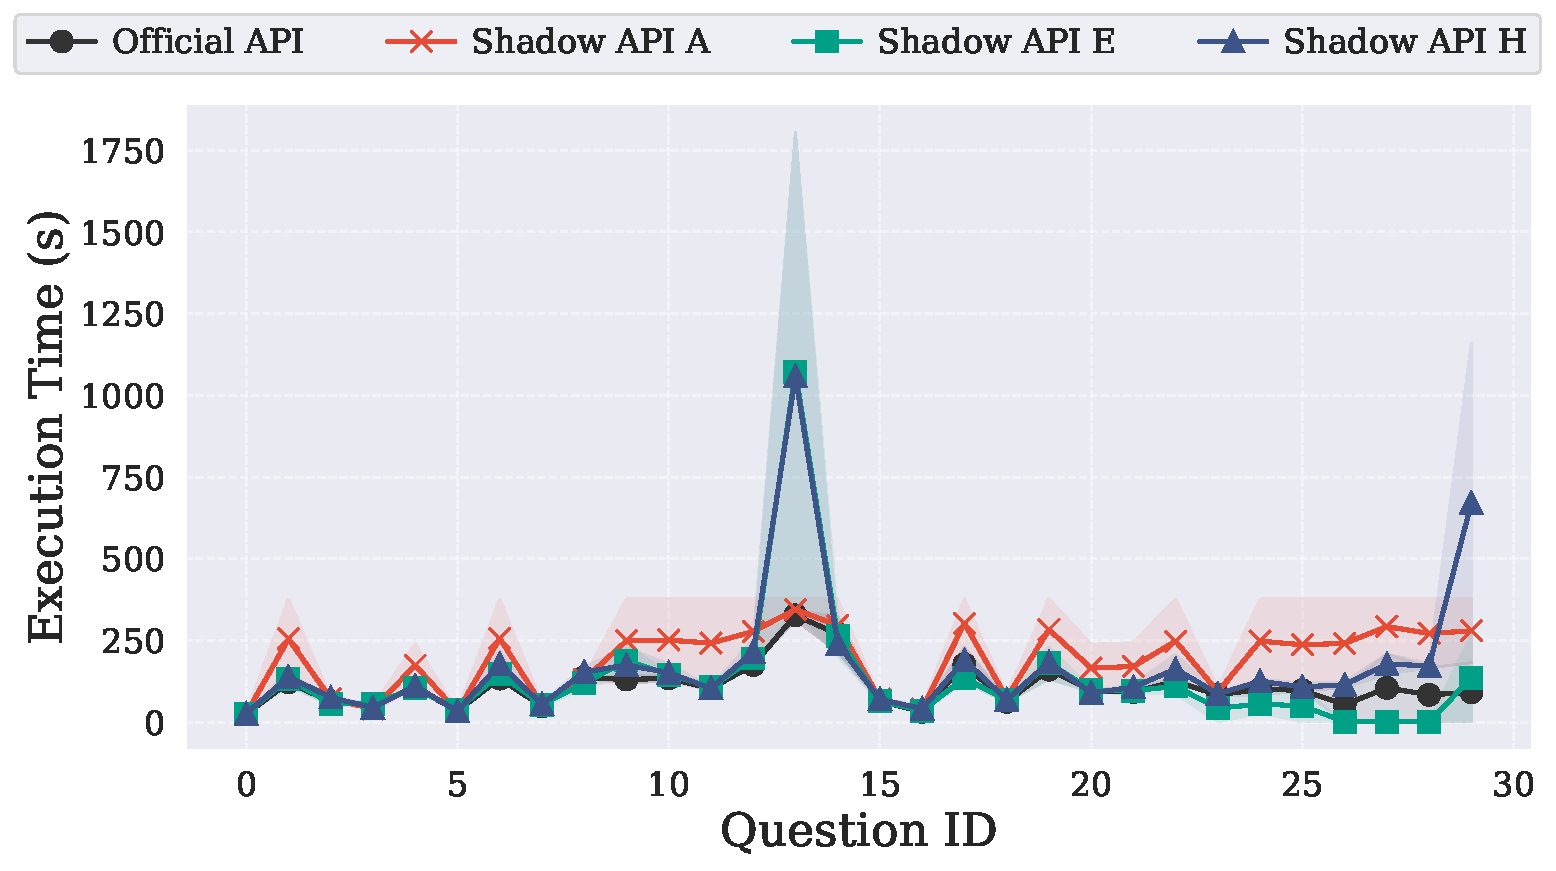
\includegraphics[width=\linewidth]{Figures/outputfig/AIME_Gemini-25-Pro_time.pdf}
        \caption{AIME: Gemini-2.5-pro (Time)}
    \end{subfigure}
    \hfill
    \begin{subfigure}{0.48\linewidth}
        \centering
        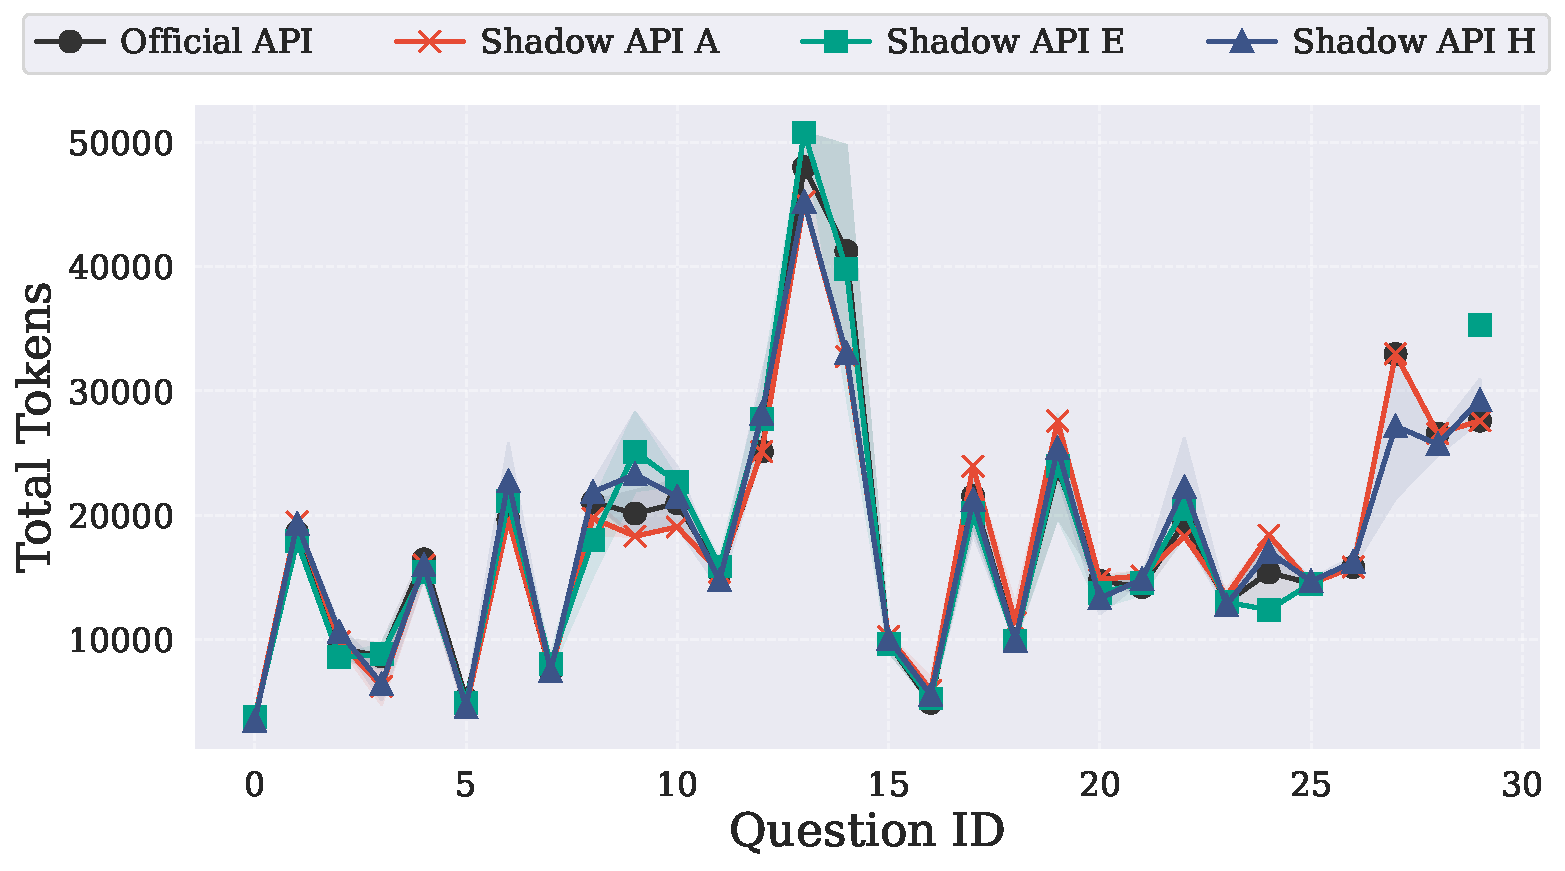
\includegraphics[width=\linewidth]{Figures/outputfig/AIME_Gemini-25-Pro_token.pdf}
        \caption{AIME: Gemini-2.5-pro (Token)}
    \end{subfigure}

    \vspace{1em}

    % --- Row 7: DeepSeek-Chat ---
    \begin{subfigure}{0.48\linewidth}
        \centering
        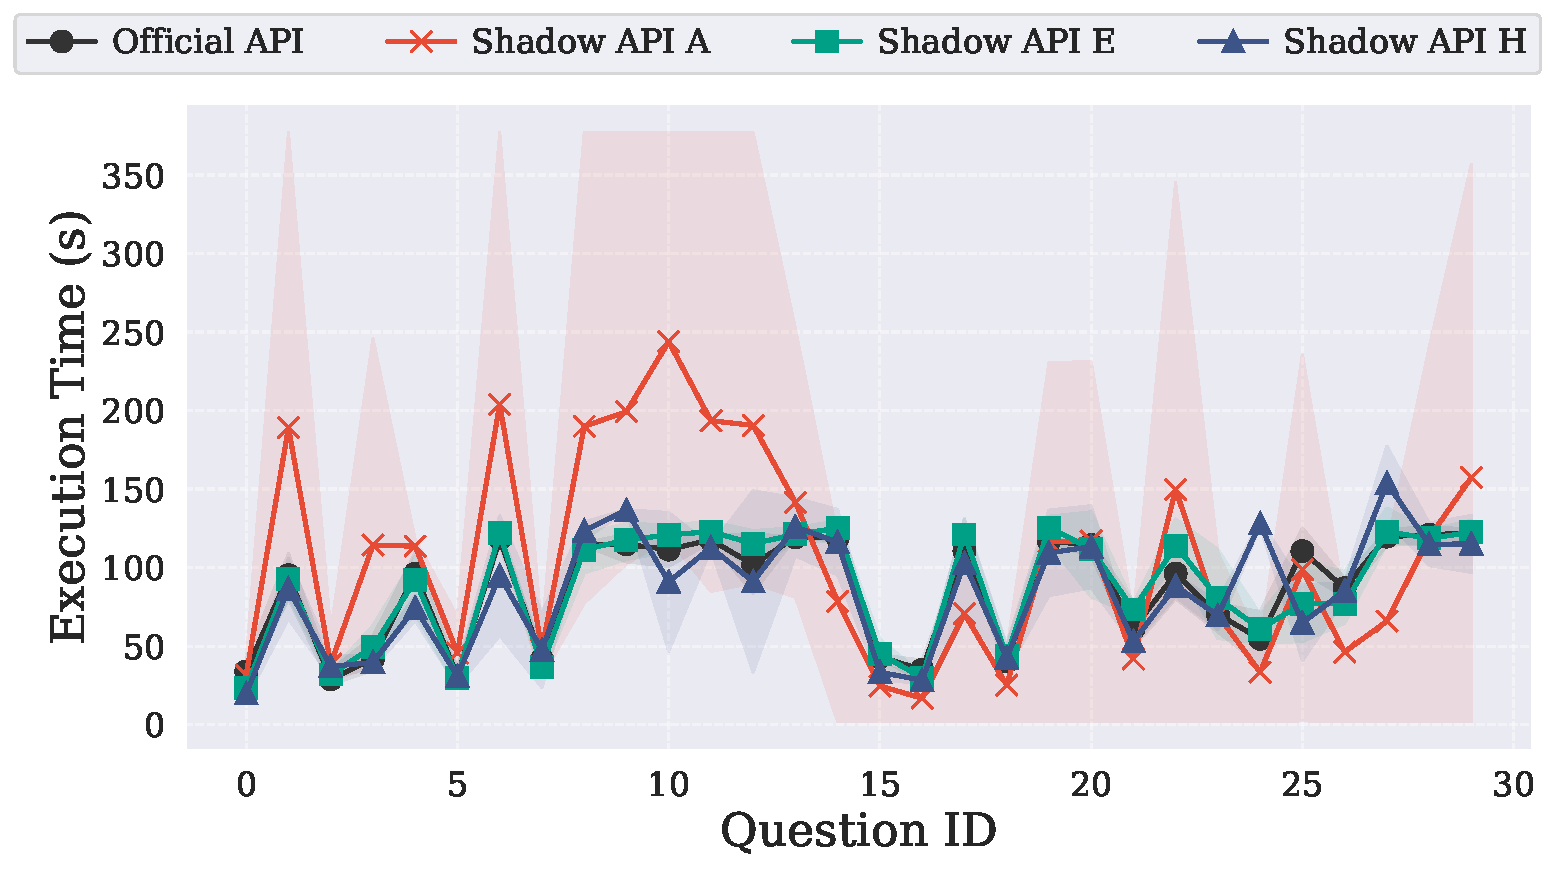
\includegraphics[width=\linewidth]{Figures/outputfig/AIME_DeepSeek-Chat_time.pdf}
        \caption{AIME: DeepSeek-Chat (Time)}
    \end{subfigure}
    \hfill
    \begin{subfigure}{0.48\linewidth}
        \centering
        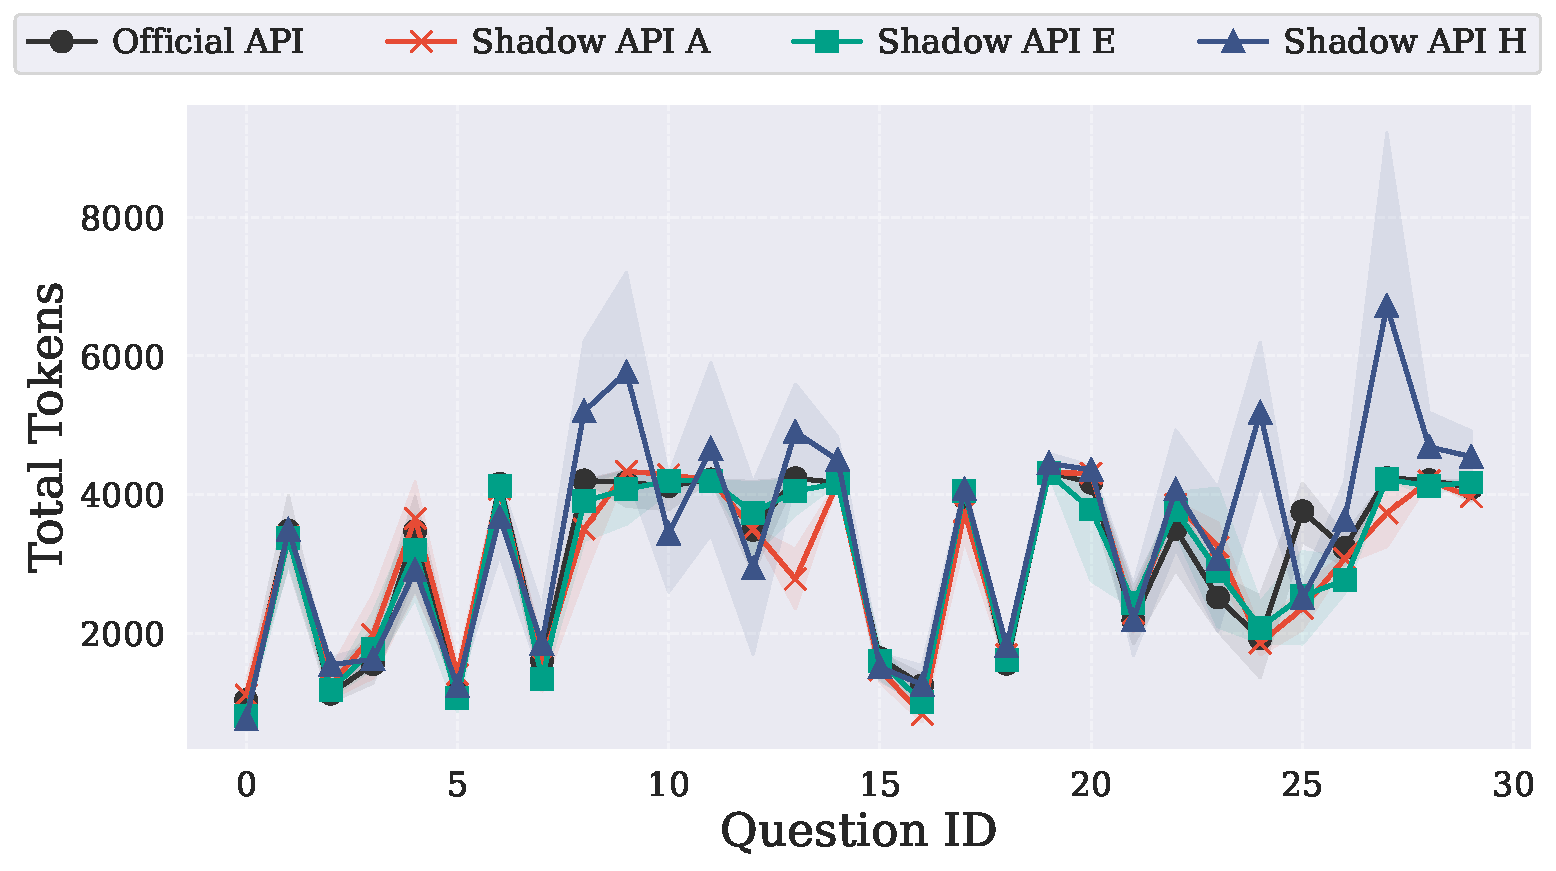
\includegraphics[width=\linewidth]{Figures/outputfig/AIME_DeepSeek-Chat_token.pdf}
        \caption{AIME: DeepSeek-Chat (Token)}
    \end{subfigure}

    \vspace{1em}

    % --- Row 8: DeepSeek-Reasoner ---
    \begin{subfigure}{0.48\linewidth}
        \centering
        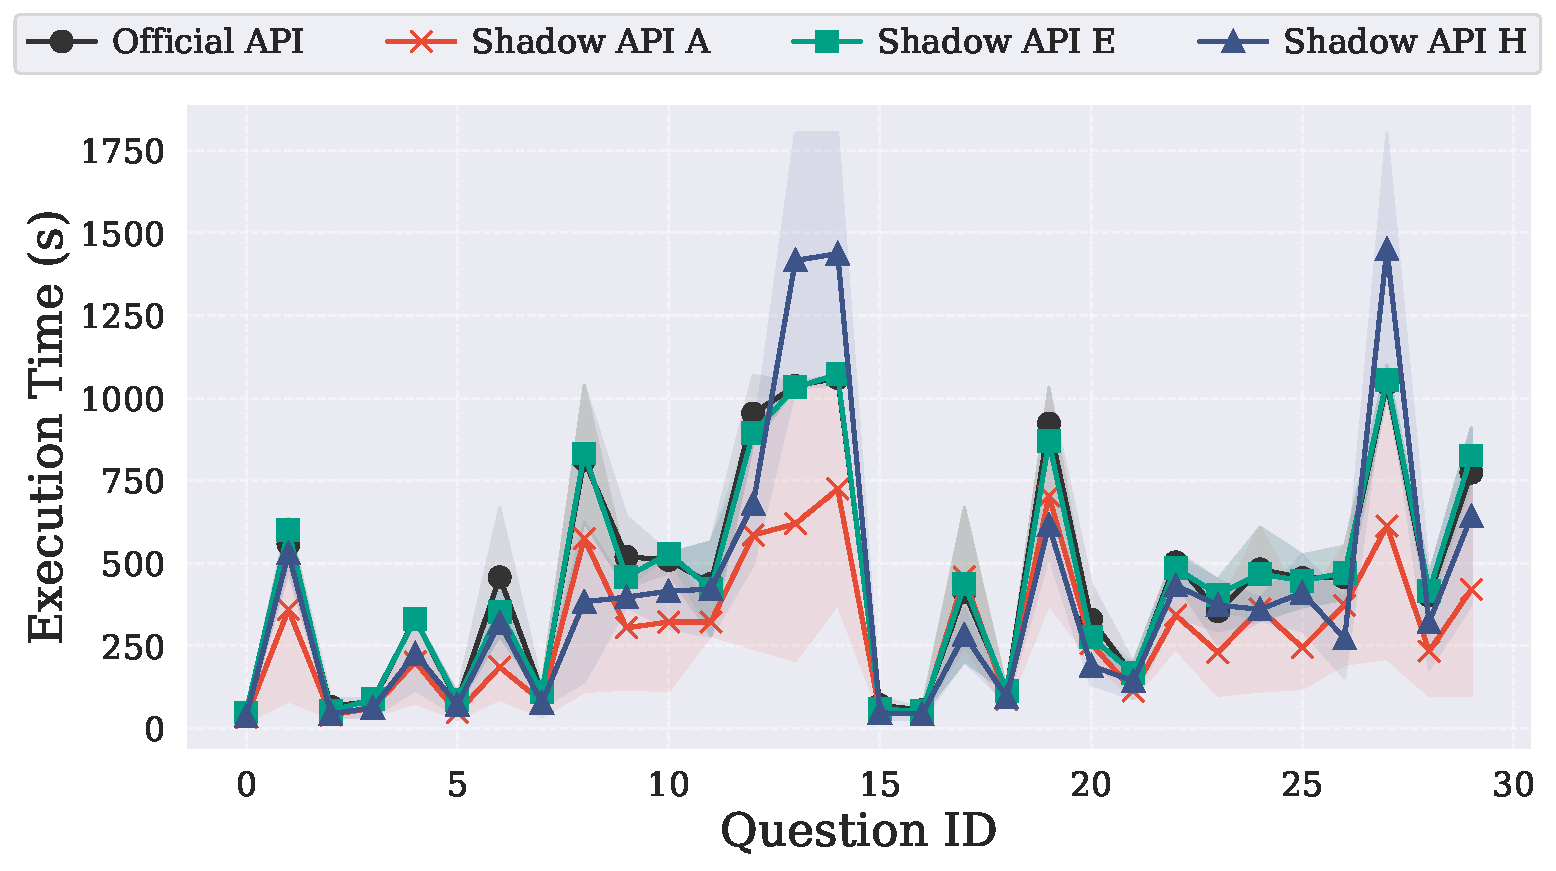
\includegraphics[width=\linewidth]{Figures/outputfig/AIME_DeepSeek-Reasoner_time.pdf}
        \caption{AIME: DeepSeek-Reasoner (Time)}
    \end{subfigure}
    \hfill
    \begin{subfigure}{0.48\linewidth}
        \centering
        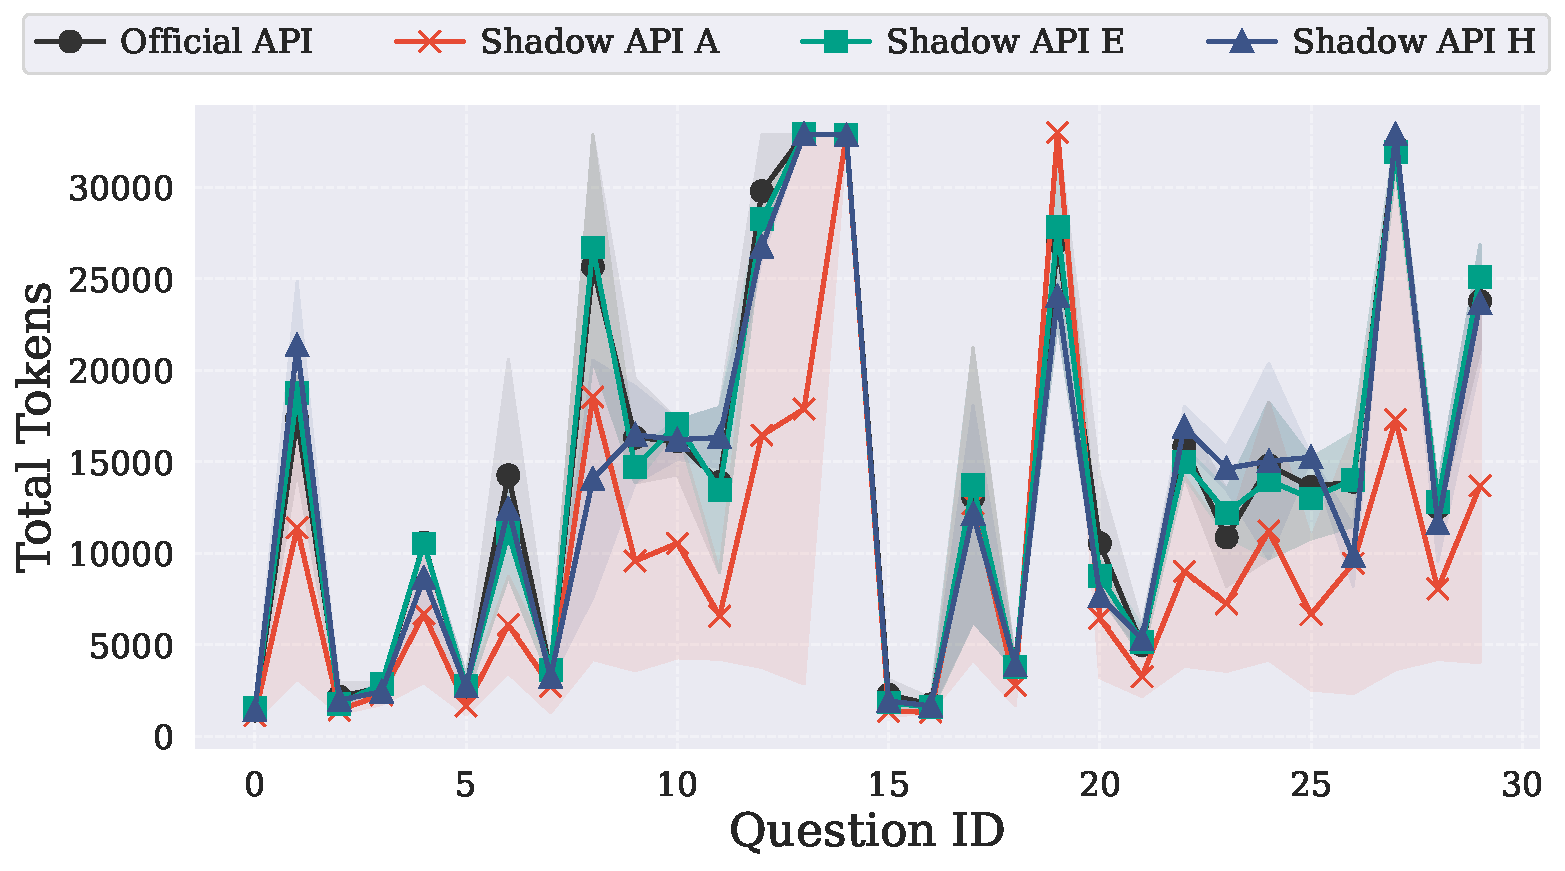
\includegraphics[width=\linewidth]{Figures/outputfig/AIME_DeepSeek-Reasoner_token.pdf}
        \caption{AIME: DeepSeek-Reasoner (Token)}
    \end{subfigure}

    \caption{Comparison of inference latency time and token counts on the AIME (Part 2).  Solid lines represent mean values, and shaded regions denote the range between the minimum and maximum values across three trials.}
    \label{fig:aime_results_part2}
\end{figure*}


\begin{figure*}[t]
    \centering
    \begin{subfigure}{0.48\linewidth}
        \centering
        \includegraphics[width=\linewidth]{Figures/outputfig/GPQA_GPT-4o-mini_time.pdf}
        \caption{GPQA: GPT-4o-mini (Time)}
    \end{subfigure}
    \hfill
    \begin{subfigure}{0.48\linewidth}
        \centering
        \includegraphics[width=\linewidth]{Figures/outputfig/GPQA_GPT-4o-mini_token.pdf}
        \caption{GPQA: GPT-4o-mini (Token)}
    \end{subfigure}

    \vspace{1em}

    % --- Row 2: GPT-5 ---
    \begin{subfigure}{0.48\linewidth}
        \centering
        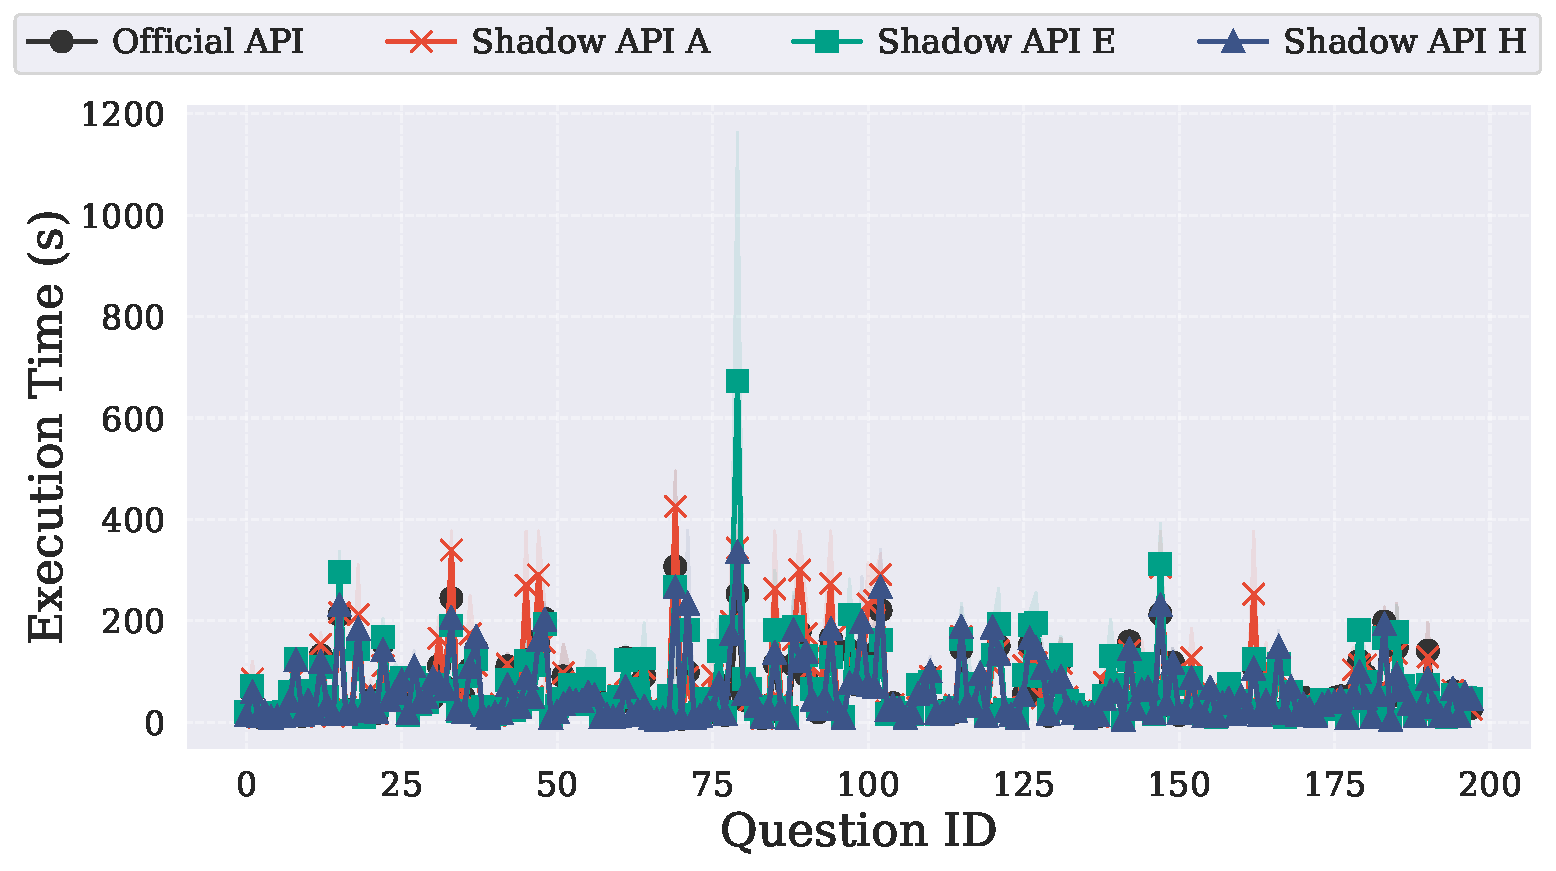
\includegraphics[width=\linewidth]{Figures/outputfig/GPQA_GPT-5_time.pdf}
        \caption{GPQA: GPT-5 (Time)}
    \end{subfigure}
    \hfill
    \begin{subfigure}{0.48\linewidth}
        \centering
        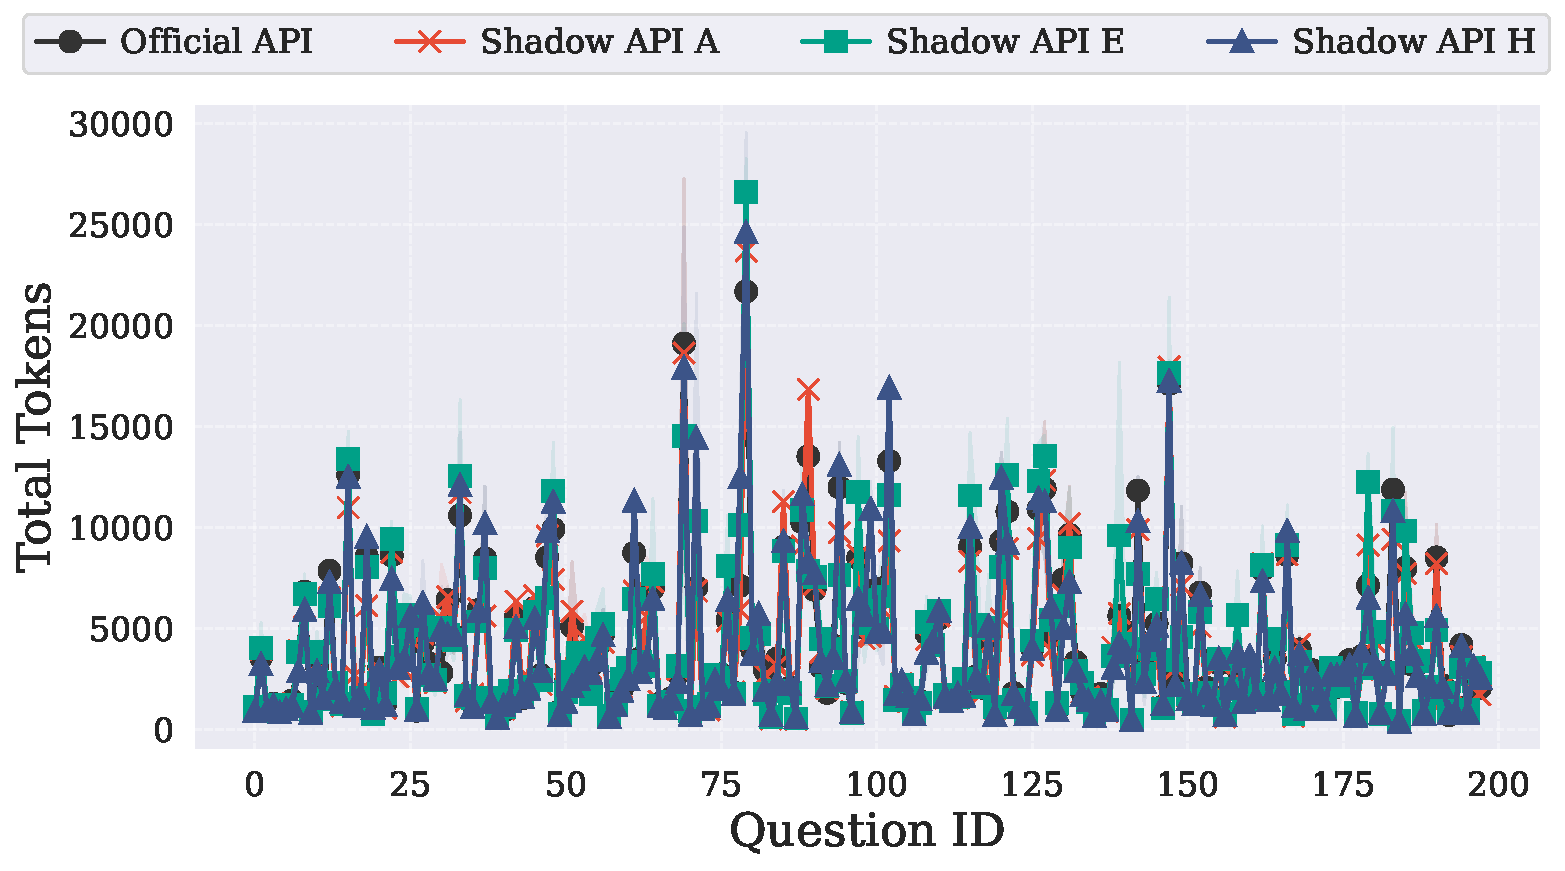
\includegraphics[width=\linewidth]{Figures/outputfig/GPQA_GPT-5_token.pdf}
        \caption{GPQA: GPT-5 (Token)}
    \end{subfigure}

    \vspace{1em}

    % --- Row 3: GPT-5-mini ---
    \begin{subfigure}{0.48\linewidth}
        \centering
        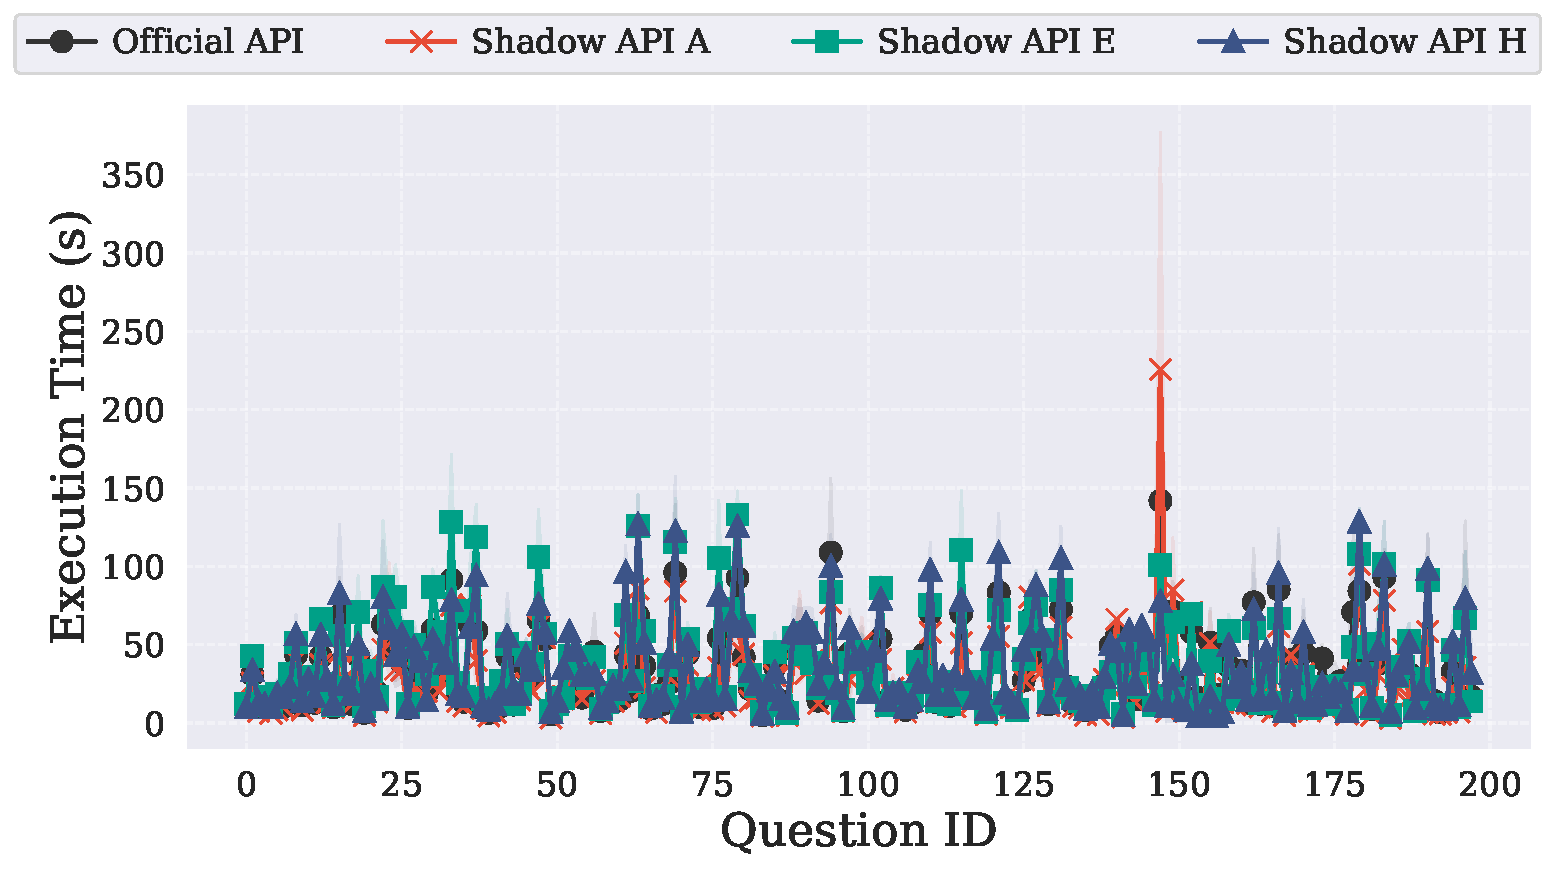
\includegraphics[width=\linewidth]{Figures/outputfig/GPQA_GPT-5-Mini_time.pdf}
        \caption{GPQA: GPT-5-mini (Time)}
    \end{subfigure}
    \hfill
    \begin{subfigure}{0.48\linewidth}
        \centering
        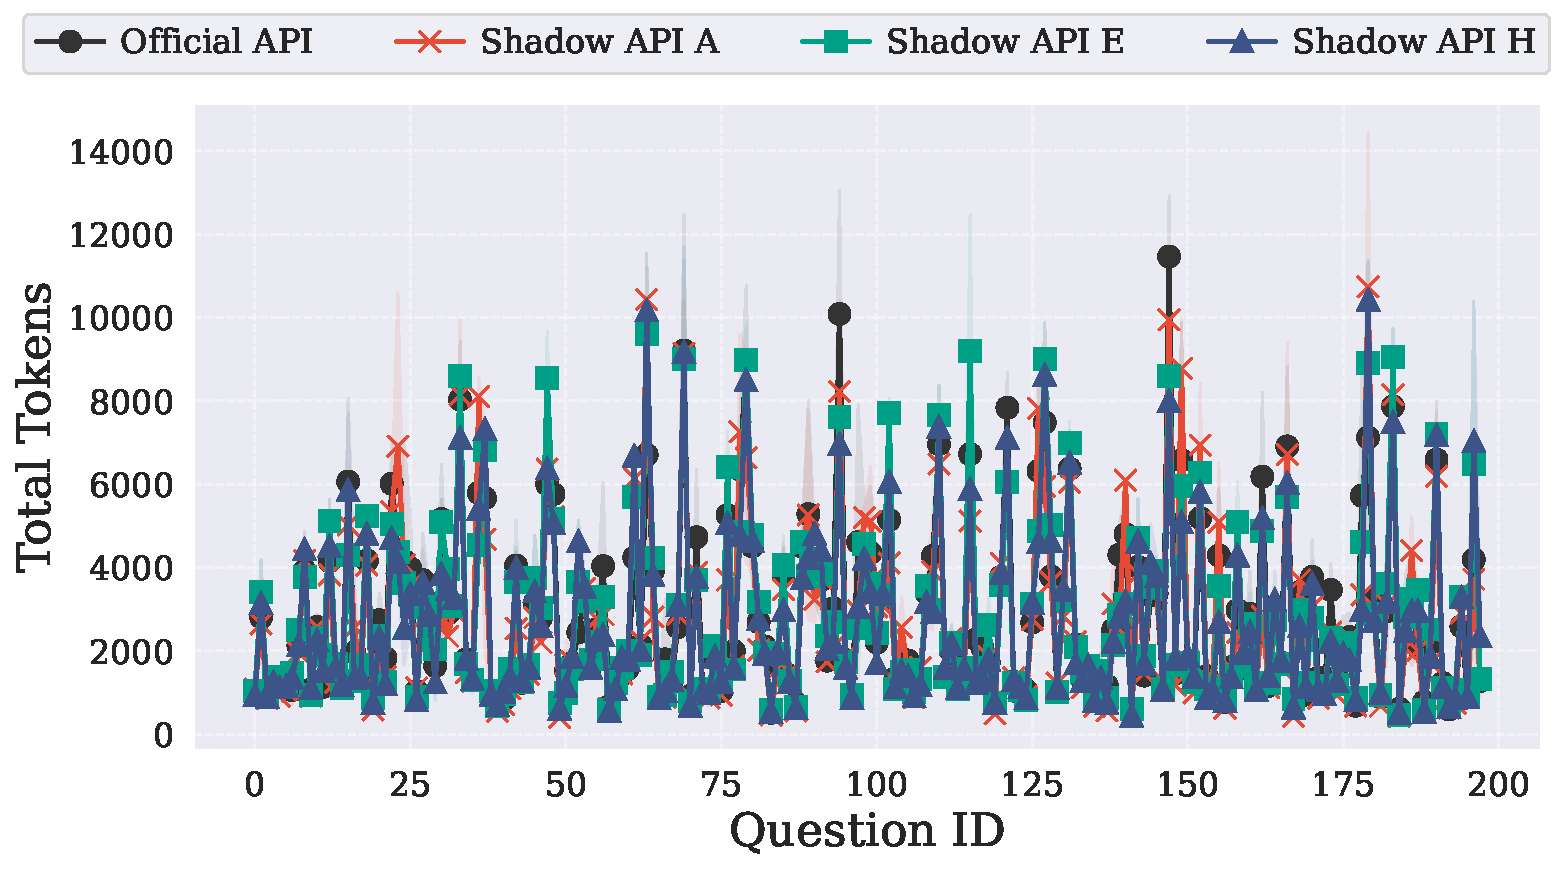
\includegraphics[width=\linewidth]{Figures/outputfig/GPQA_GPT-5-Mini_token.pdf}
        \caption{GPQA: GPT-5-mini (Token)}
    \end{subfigure}

    \vspace{1em}

    % --- Row 4: Gemini-2.0-flash ---
    \begin{subfigure}{0.48\linewidth}
        \centering
        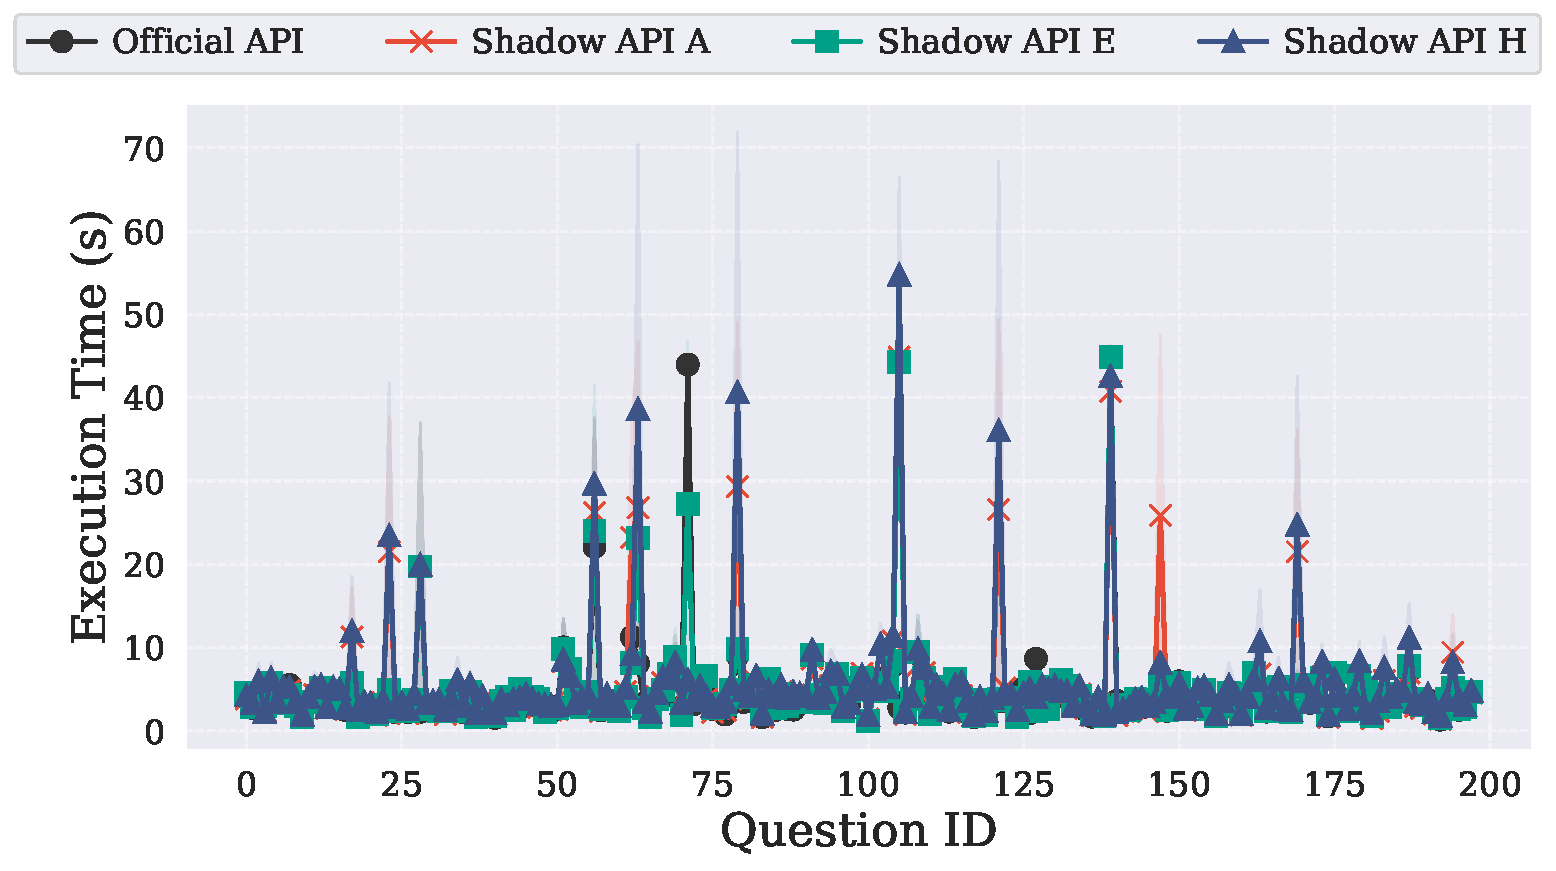
\includegraphics[width=\linewidth]{Figures/outputfig/GPQA_Gemini-20-Flash_time.pdf}
        \caption{GPQA: Gemini-2.0-flash (Time)}
    \end{subfigure}
    \hfill
    \begin{subfigure}{0.48\linewidth}
        \centering
        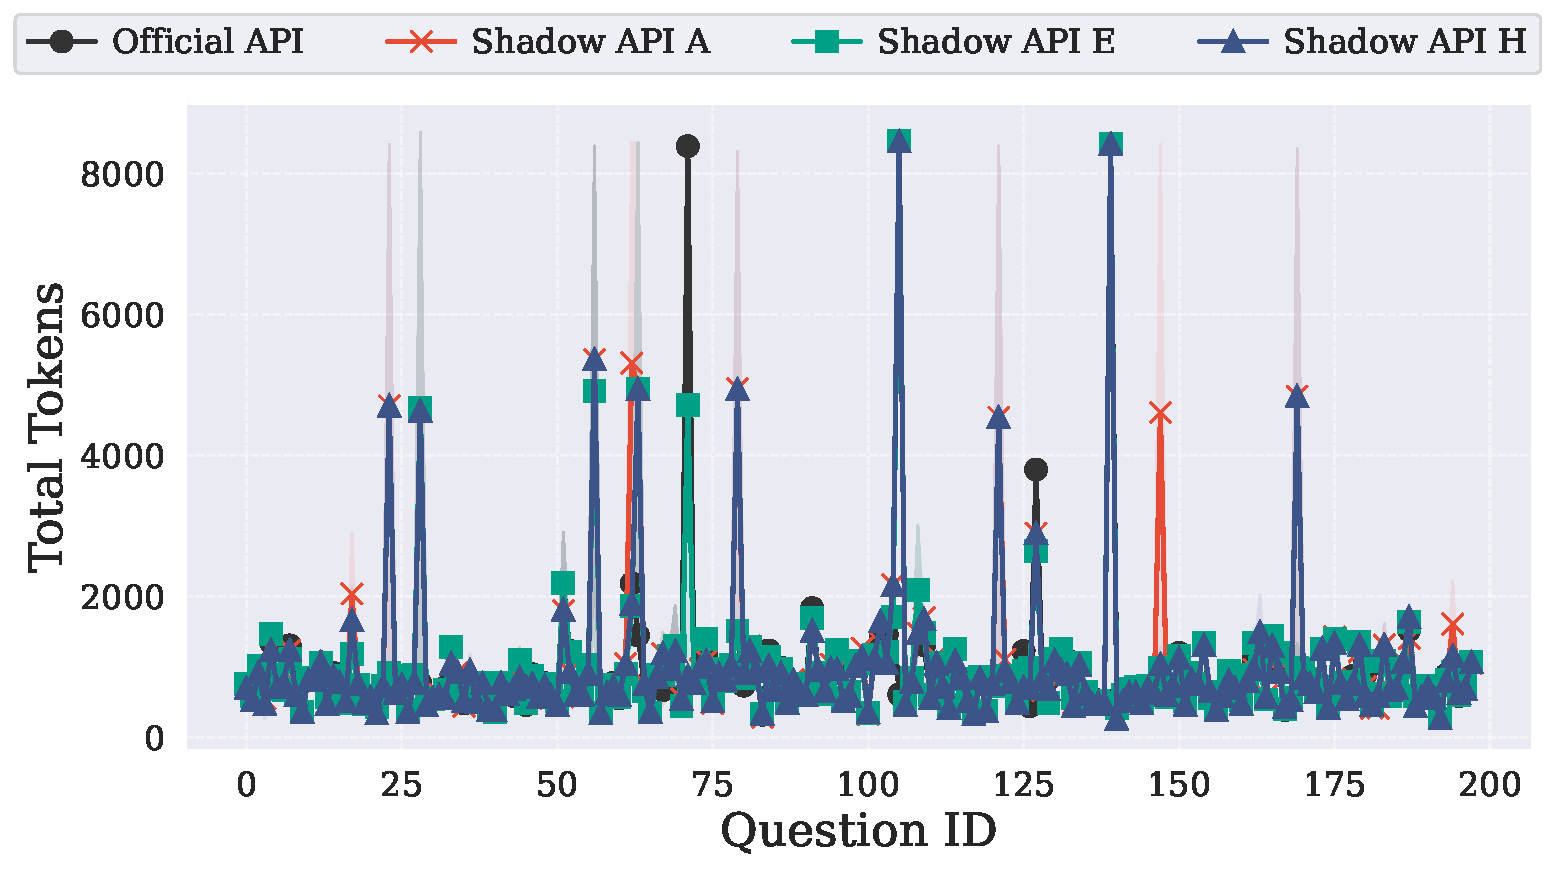
\includegraphics[width=\linewidth]{Figures/outputfig/GPQA_Gemini-20-Flash_token.pdf}
        \caption{GPQA: Gemini-2.0-flash (Token)}
    \end{subfigure}
    \caption{Comparison of inference latency time and token counts on the GPQA (Part 1).  Solid lines represent mean values, and shaded regions denote the range between the minimum and maximum values across three trials.}
    \label{figure:gpqa_part1}
\end{figure*}

\begin{figure*}[t]
    \centering

    % --- Row 5: Gemini-2.5-flash ---
    \begin{subfigure}{0.48\linewidth}
        \centering
        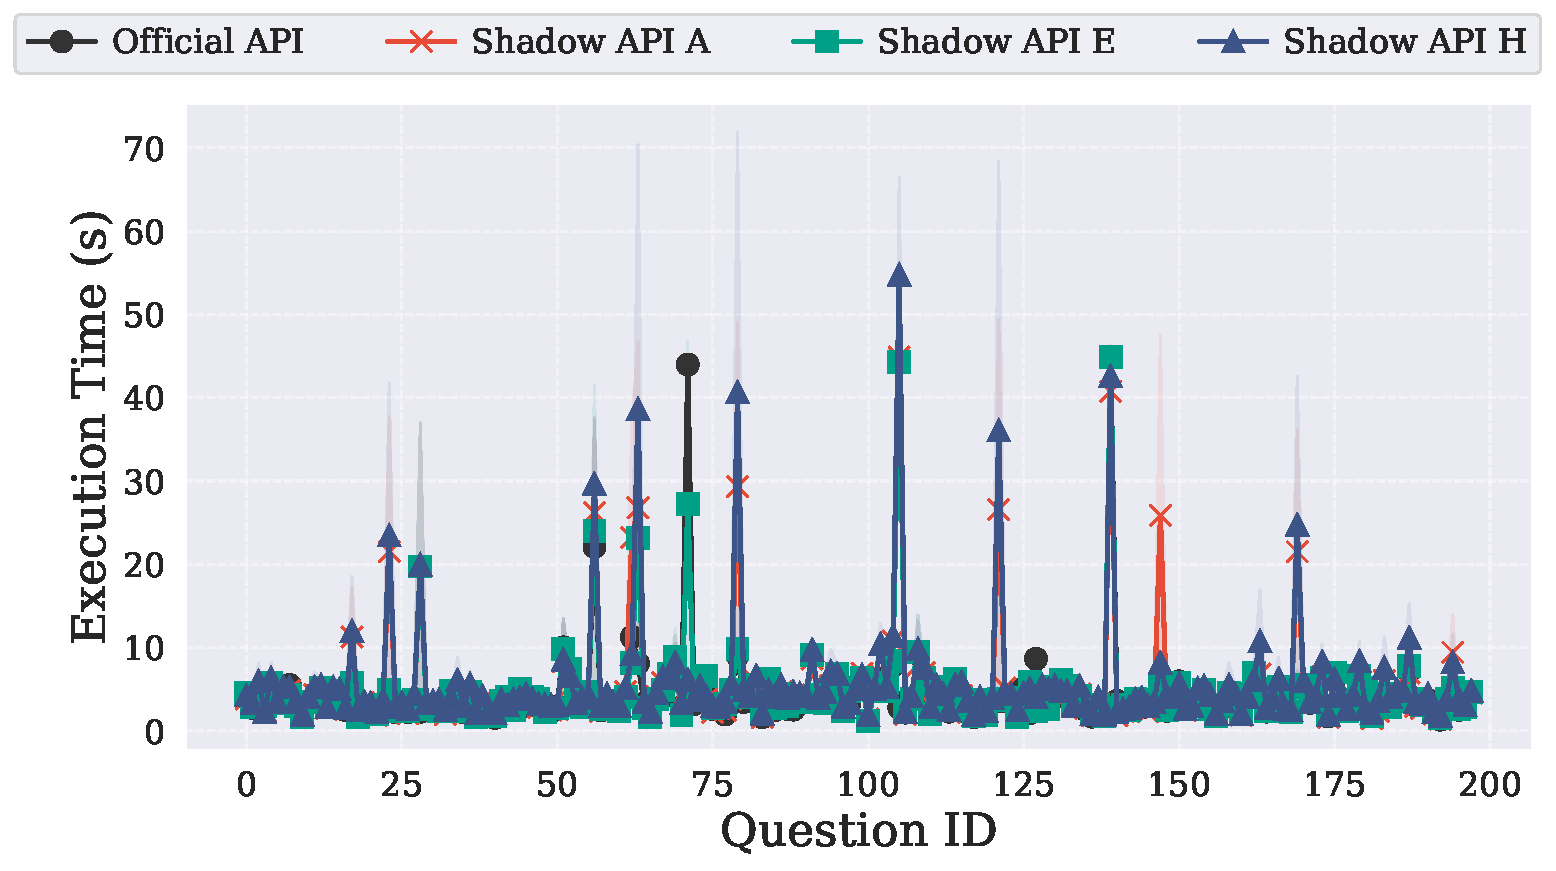
\includegraphics[width=\linewidth]{Figures/outputfig/GPQA_Gemini-25-Flash_time.pdf}
        \caption{GPQA: Gemini-2.5-flash (Time)}
    \end{subfigure}
    \hfill
    \begin{subfigure}{0.48\linewidth}
        \centering
        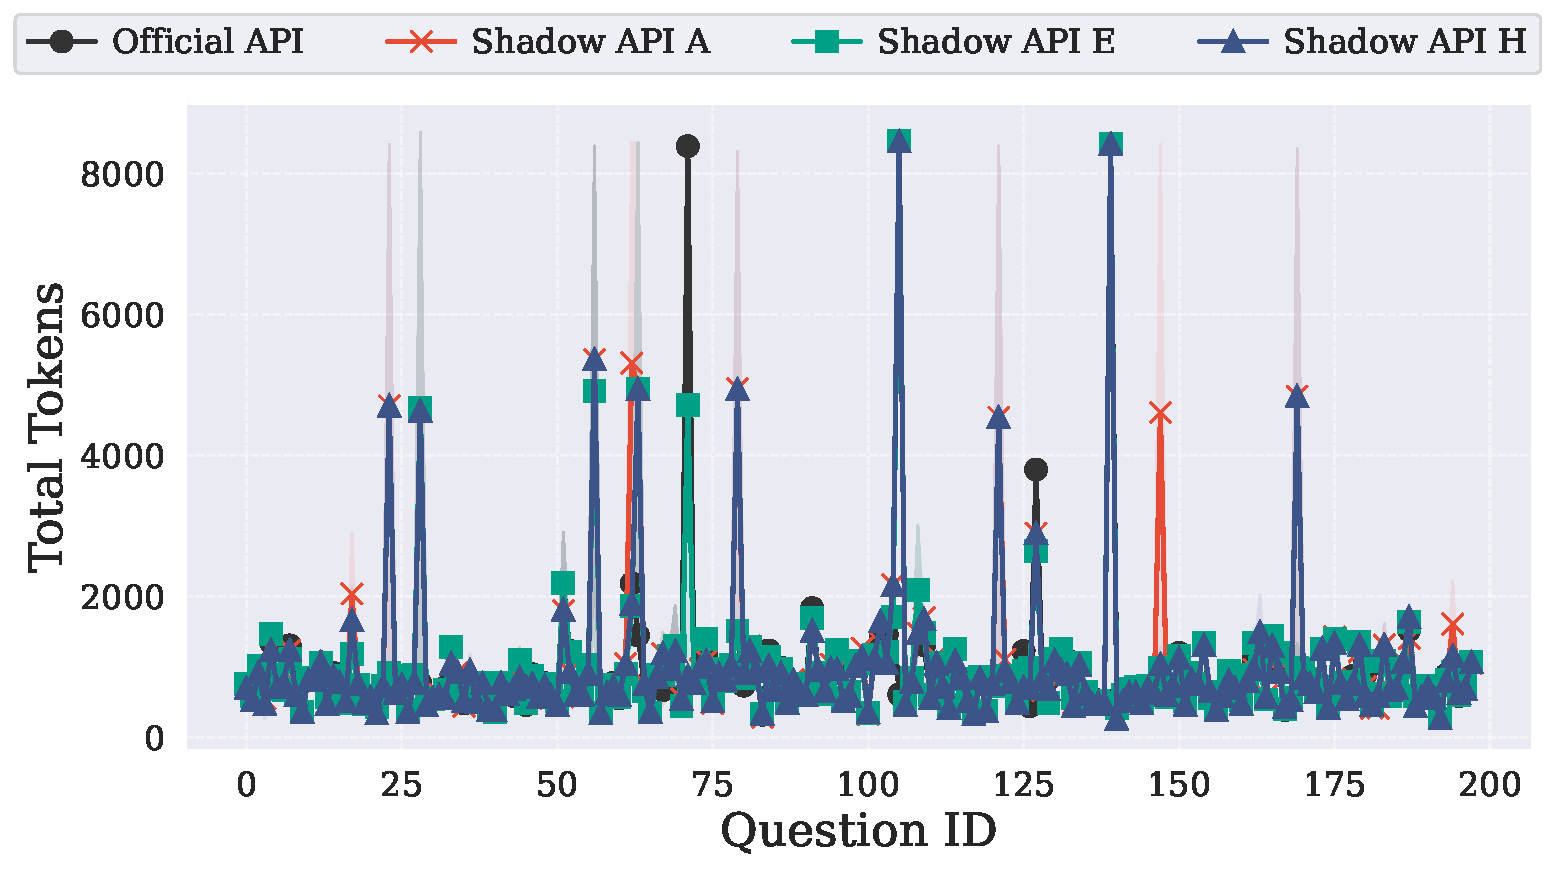
\includegraphics[width=\linewidth]{Figures/outputfig/GPQA_Gemini-25-Flash_token.pdf}
        \caption{GPQA: Gemini-2.5-flash (Token)}
    \end{subfigure}

    \vspace{1em}

    % --- Row 6: Gemini-2.5-pro ---
    \begin{subfigure}{0.48\linewidth}
        \centering
        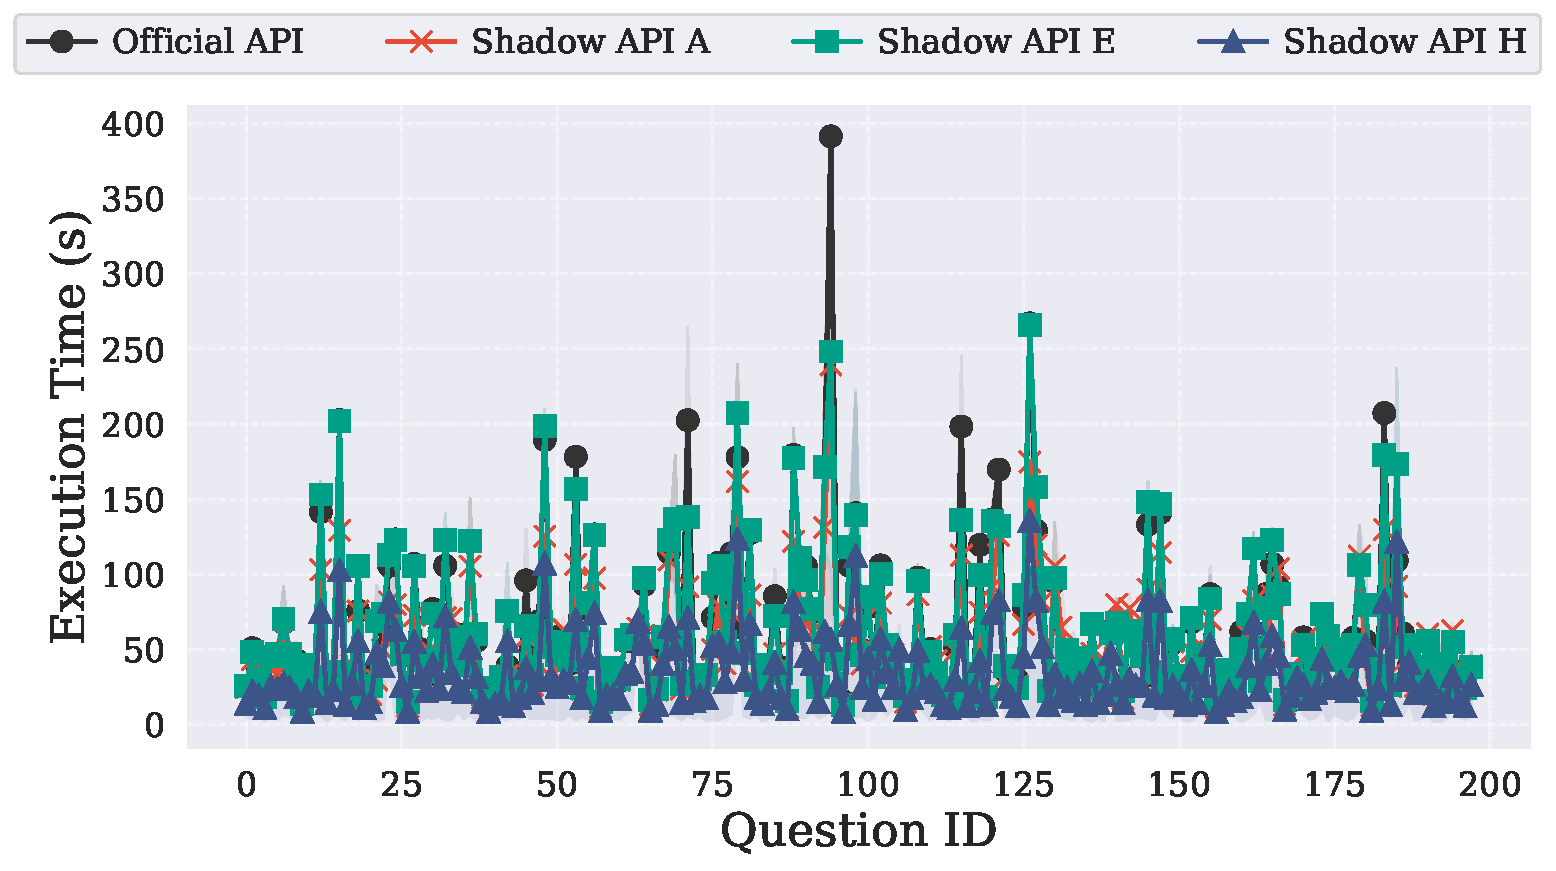
\includegraphics[width=\linewidth]{Figures/outputfig/GPQA_Gemini-25-Pro_time.pdf}
        \caption{GPQA: Gemini-2.5-pro (Time)}
    \end{subfigure}
    \hfill
    \begin{subfigure}{0.48\linewidth}
        \centering
        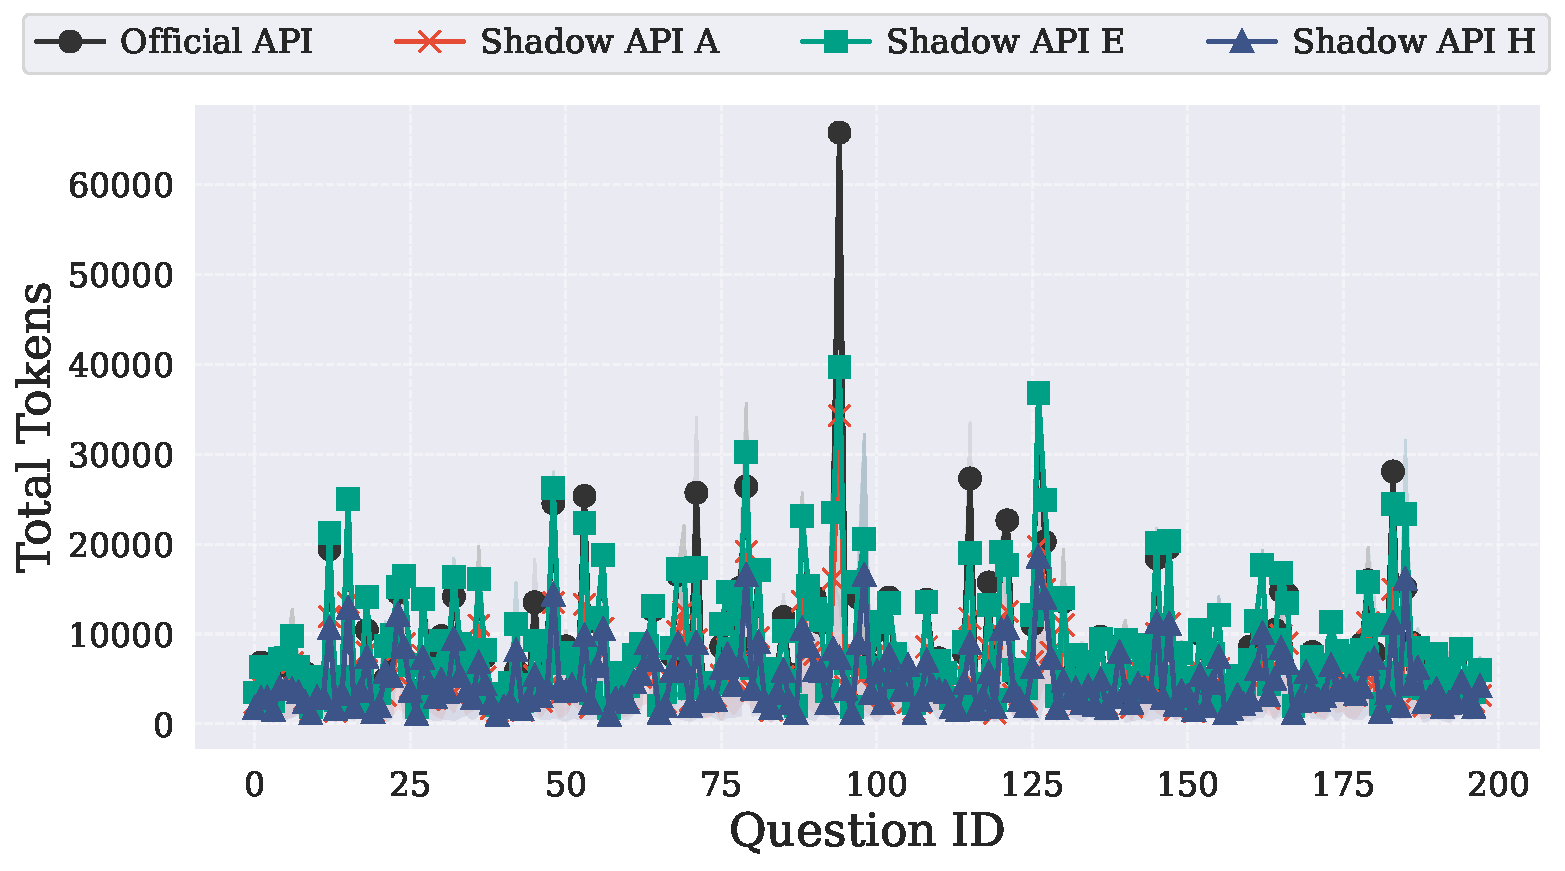
\includegraphics[width=\linewidth]{Figures/outputfig/GPQA_Gemini-25-Pro_token.pdf}
        \caption{GPQA: Gemini-2.5-pro (Token)}
    \end{subfigure}

    \vspace{1em}

    % --- Row 7: DeepSeek-Chat ---
    \begin{subfigure}{0.48\linewidth}
        \centering
        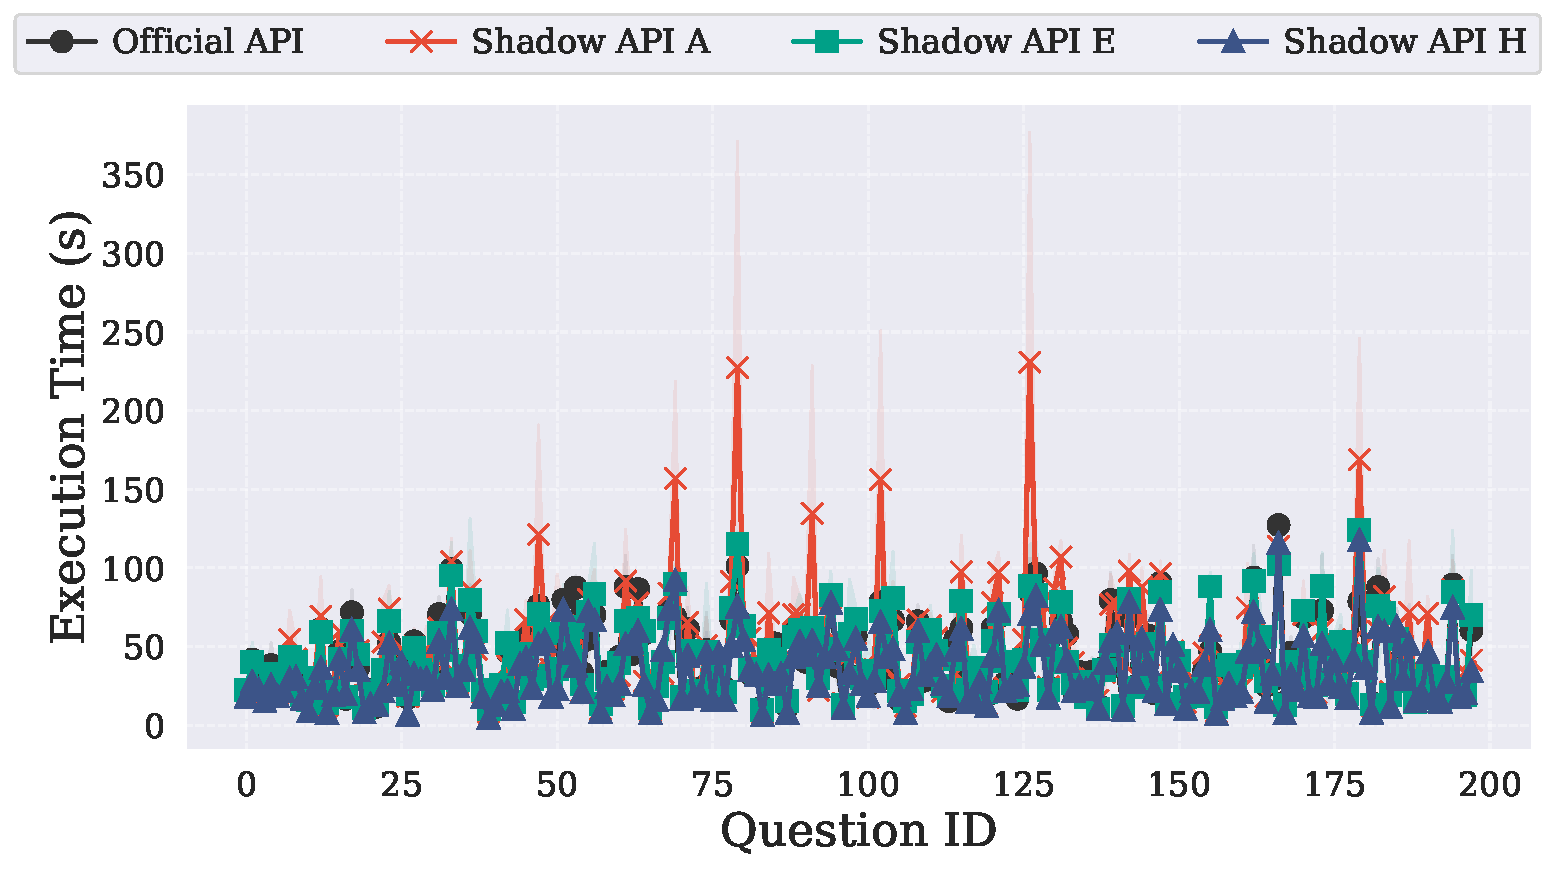
\includegraphics[width=\linewidth]{Figures/outputfig/GPQA_DeepSeek-Chat_time.pdf}
        \caption{GPQA: DeepSeek-Chat (Time)}
    \end{subfigure}
    \hfill
    \begin{subfigure}{0.48\linewidth}
        \centering
        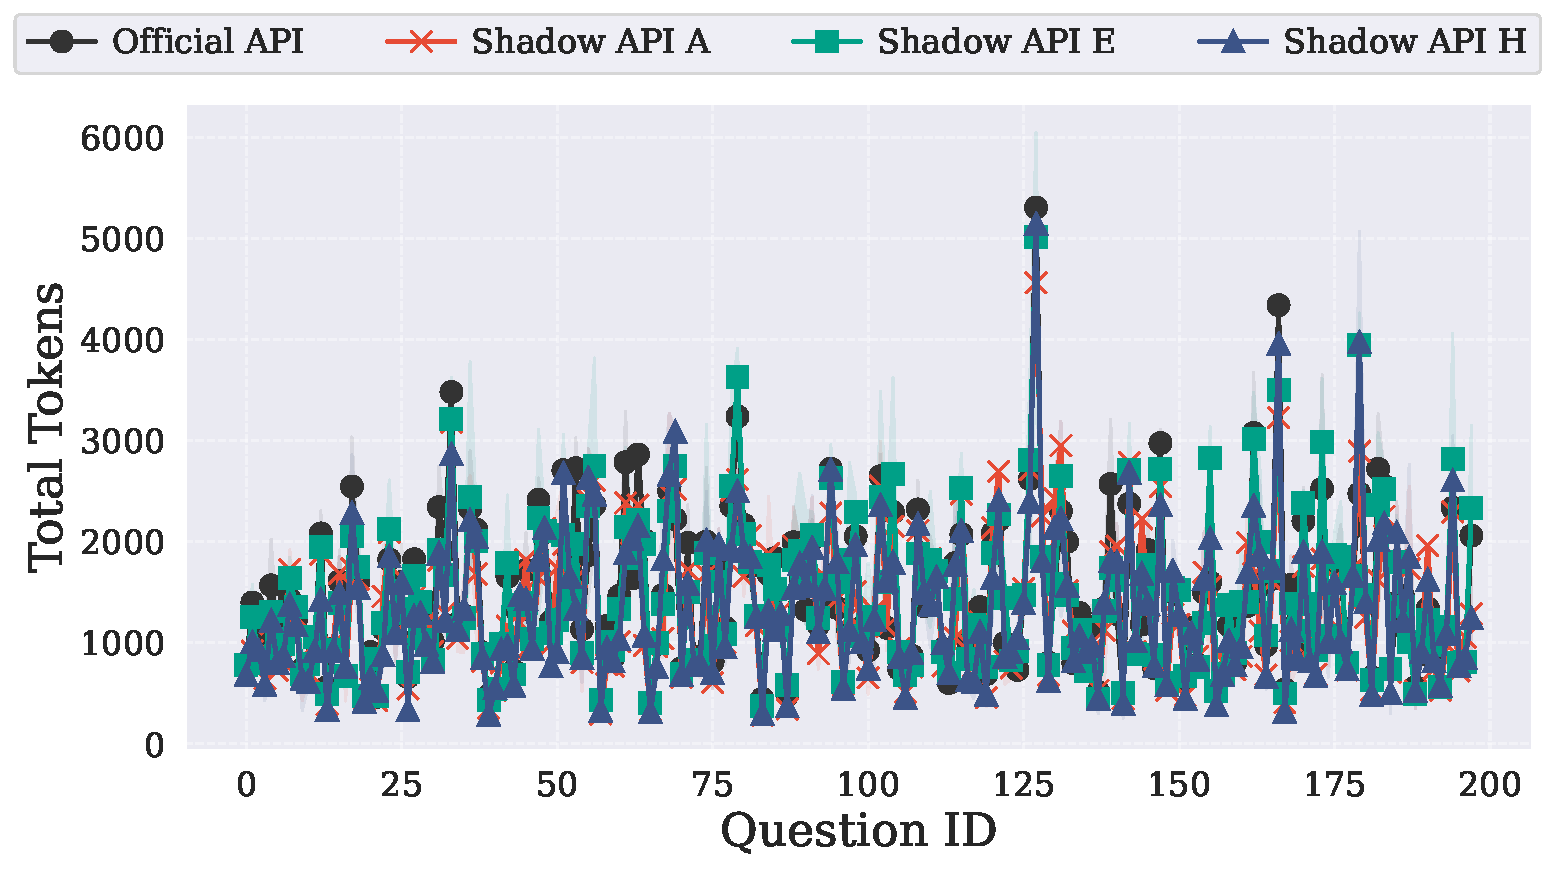
\includegraphics[width=\linewidth]{Figures/outputfig/GPQA_DeepSeek-Chat_token.pdf}
        \caption{GPQA: DeepSeek-Chat (Token)}
    \end{subfigure}

    \vspace{1em}

    % --- Row 8: DeepSeek-Reasoner ---
    \begin{subfigure}{0.48\linewidth}
        \centering
        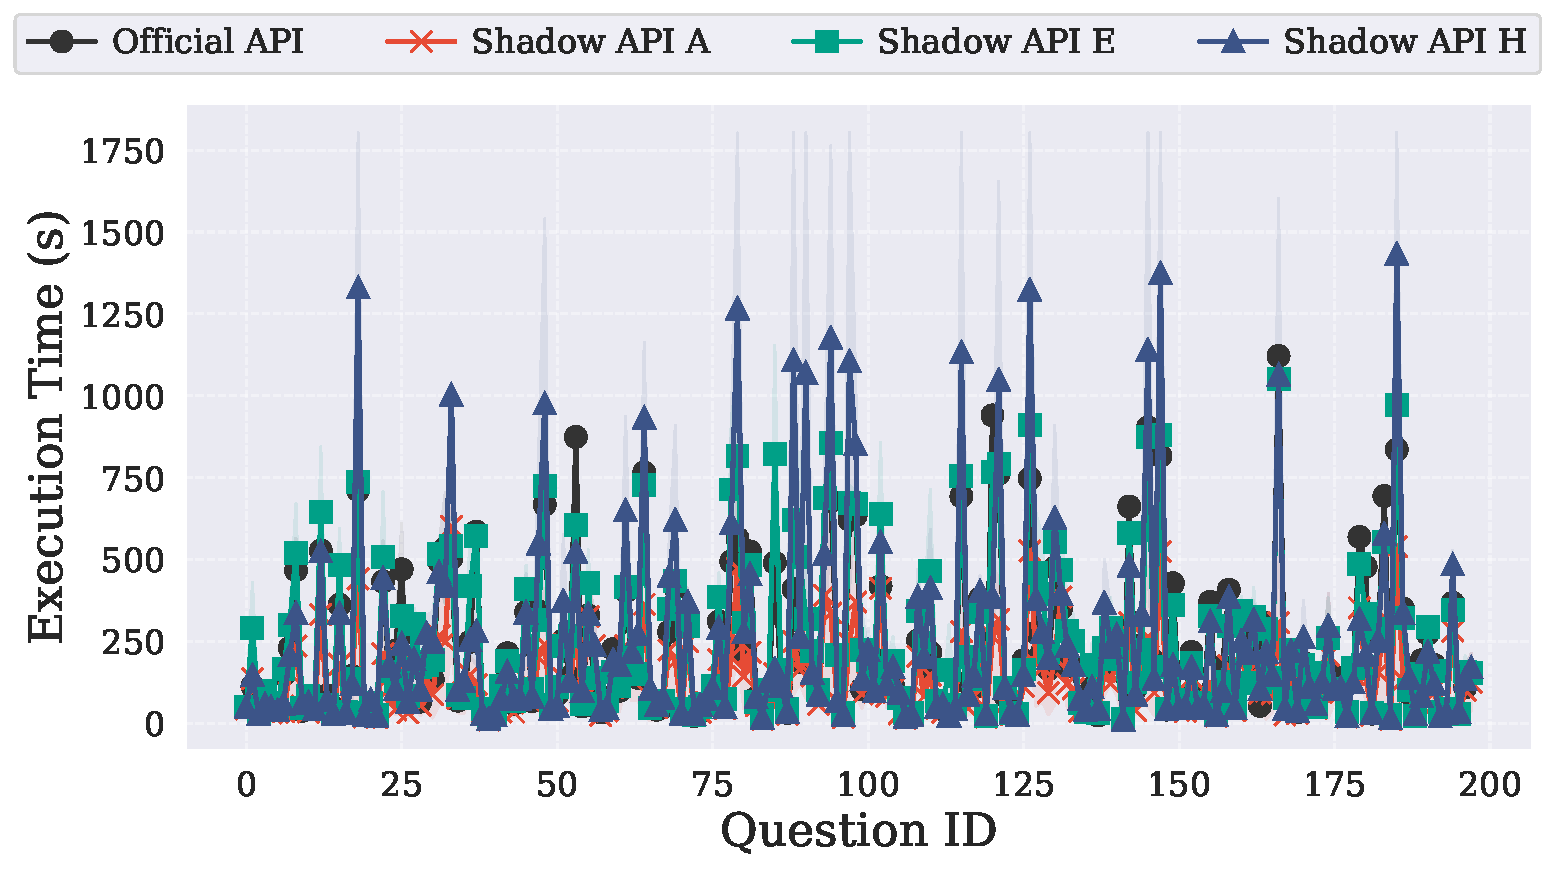
\includegraphics[width=\linewidth]{Figures/outputfig/GPQA_DeepSeek-Reasoner_time.pdf}
        \caption{GPQA: DeepSeek-Reasoner (Time)}
    \end{subfigure}
    \hfill
    \begin{subfigure}{0.48\linewidth}
        \centering
        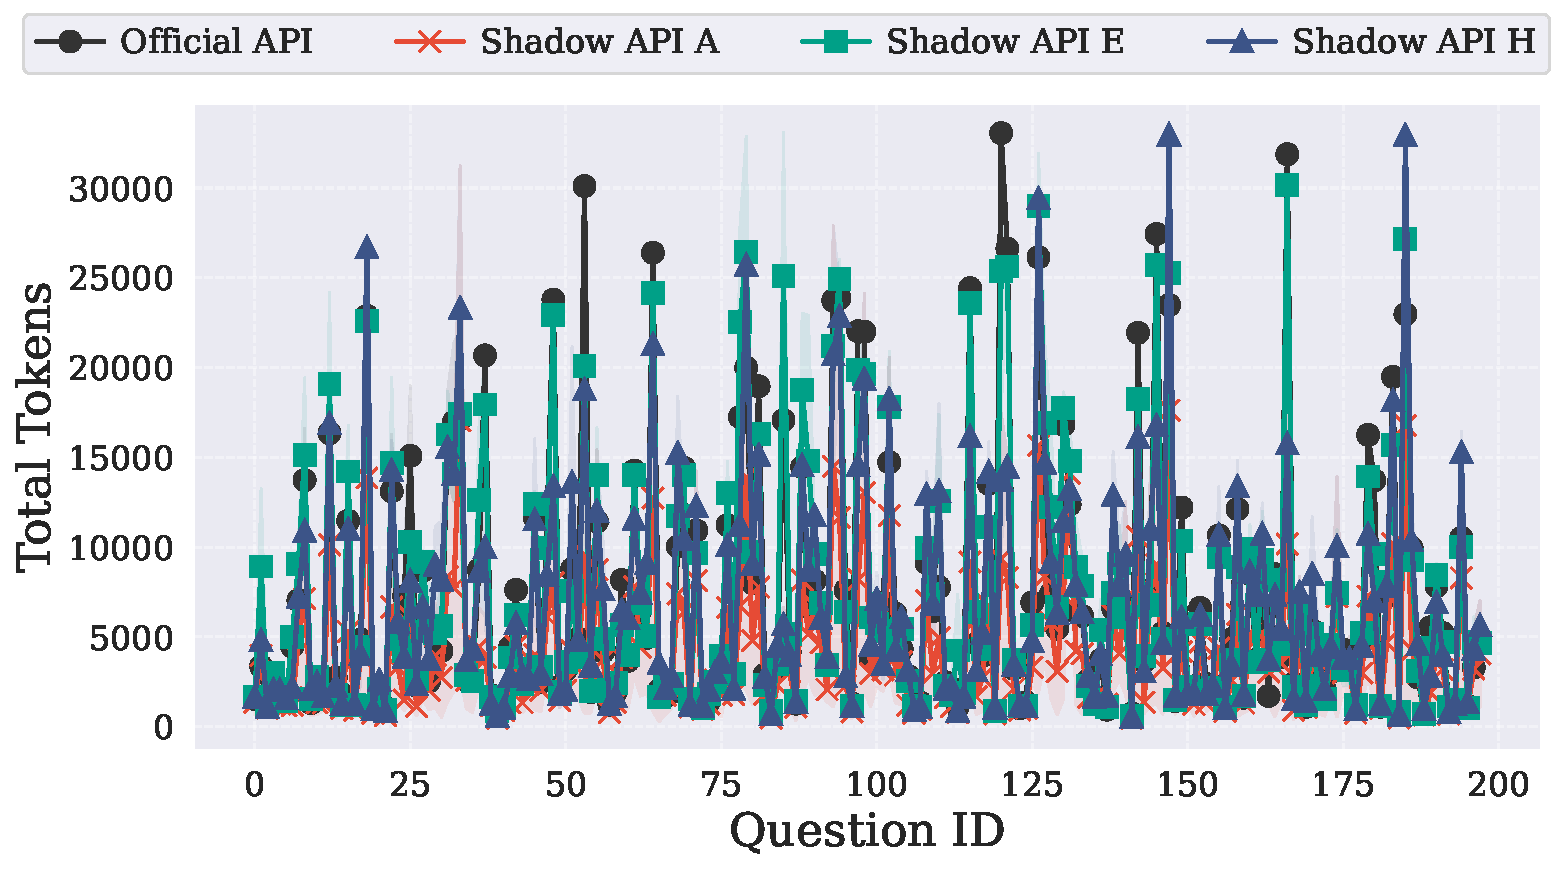
\includegraphics[width=\linewidth]{Figures/outputfig/GPQA_DeepSeek-Reasoner_token.pdf}
        \caption{GPQA: DeepSeek-Reasoner (Token)}
    \end{subfigure}

    \caption{Comparison of inference latency time and token counts on the GPQA (Part 2). Solid lines represent mean values, and shaded regions denote the range between the minimum and maximum values across three trials.}
    \label{fig:gpqa_results_part2}
\end{figure*}

%-------------------------------------------------------------------------------
\section{LLMs Used for Training LLMmap}
\label{appendix:llmmap_model}
%-------------------------------------------------------------------------------

\autoref{table: models} provides a comprehensive inventory of the LLMs utilized in this study, distinguishing between the original baseline models and newly integrated trained models.
All officially trained models are queried directly through the corresponding official APIs.

%-------------------------------------------------------------------------------
\begin{table*}[ht!]
\centering
\caption{Controlled validation scenarios. Each scenario contains $N{=}100$ samples.}
\label{tab:validation_scenarios}
\scalebox{0.9}{
\begin{tabular}{llll}
\toprule
\textbf{Type} & \textbf{Claimed Model} & \textbf{Ground Truth Backend} & \textbf{Simulated Behavior} \\
\midrule
Honest    & GPT-5                & GPT-5                  & ---                    \\
Honest    & Gemini-2.0-flash     & Gemini-2.0-flash       & ---                    \\
Honest    & DeepSeek-Reasoner    & DeepSeek-Reasoner      & ---                    \\
Deceptive & GPT-5                & GLM-4-9B               & Model substitution     \\
Deceptive & Gemini-2.0-flash     & Gemini-2.5-flash       & Version mismatch       \\
Deceptive & DeepSeek-Reasoner    & DeepSeek-Chat          & Capability downgrading \\
\bottomrule
\end{tabular}
}
\end{table*}
%-------------------------------------------------------------------------------

%-------------------------------------------------------------------------------
\begin{table}[ht!]
\centering
\caption{LLMmap accuracy on the controlled validation testbed.}
\label{tab:validation_llmmap}
\scalebox{0.9}{
\begin{tabular}{lccc}
\toprule
\textbf{Model Family} & \textbf{Acc} & \textbf{FPR} & \textbf{FNR} \\
\midrule
GPT family      & 96.00\% & 3.00\% & 5.00\% \\
Gemini family   & 96.00\% & 2.00\% & 6.00\% \\
DeepSeek family & 96.00\% & 4.00\% & 4.00\% \\
\midrule
\textbf{Overall} & \textbf{96.00\%} & \textbf{3.00\%} & \textbf{5.00\%} \\
\bottomrule
\end{tabular}
}
\end{table}
%-------------------------------------------------------------------------------

%-------------------------------------------------------------------------------
\begin{table}[ht!]
\centering
\caption{MET accuracy on the controlled validation testbed.}
\label{tab:validation_met}
\scalebox{0.9}{
\begin{tabular}{lccc}
\toprule
\textbf{Model Family} & \textbf{Acc} & \textbf{FPR} & \textbf{FNR} \\
\midrule
GPT family      & 88.50\% & 5.00\% & 18.00\% \\
Gemini family   & 87.00\% & 5.00\% & 21.00\% \\
DeepSeek family & 89.50\% & 4.00\% & 17.00\% \\
\midrule
\textbf{Overall} & \textbf{88.33\%} & \textbf{4.67\%} & \textbf{18.67\%} \\
\bottomrule
\end{tabular}
}
\end{table}
%-------------------------------------------------------------------------------

%-------------------------------------------------------------------------------
\begin{table}[ht!]
\centering
\caption{OLS regression predicting accuracy drop ($\Delta\text{acc}$) across 24 shadow API endpoints.}
\label{tab:regression}
\scalebox{0.9}{
\begin{tabular}{lrrrr}
\toprule
\textbf{Variable} & \textbf{$\beta$} & \textbf{$SE$} & \textbf{$t$} & \textbf{$p$} \\
\midrule
Cosine Distance   & $-0.385$ & $1.412$ & $-0.272$ & $0.789$ \\
Price Ratio       & $-1.447$ & $2.055$ & $-0.704$ & $0.490$ \\
Identity Mismatch & $0.224$  & $7.250$ & $0.031$  & $0.976$ \\
Reasoning Model   & $10.092$ & $7.537$ & $1.339$  & $0.197$ \\
\midrule
\multicolumn{5}{l}{$R^2 = 0.153$, $n = 24$} \\
\bottomrule
\end{tabular}
}
\end{table}
%-------------------------------------------------------------------------------

%-------------------------------------------------------------------------------
\begin{table*}[t]
\centering
\caption{List of LLMs used for training and testing LLMmap. The table is divided into the original baseline models and additionally trained models.}
\footnotesize

\scalebox{0.9}{
\begin{tabular}{llcc}
\toprule
\textbf{\#} & \textbf{Version} & \textbf{Provider} & \textbf{Number of Parameters} \\ 
\midrule
\multicolumn{4}{c}{\textit{\textbf{Part I: Original Trained Models}}} \\
\midrule
1 & ChatGPT-3.5 (gpt-3.5-turbo-0125) & OpenAI & / \\ \hline
2 & ChatGPT-4  (gpt-4-turbo-2024-04-09) & OpenAI & / \\ \hline
3 & ChatGPT-4o (gpt-4o-2024-05-13) & OpenAI & / \\ \hline
4 & Claude 3 Haiku (claude-3-haiku-20240307) & Anthropic & / \\ \hline
5 & Claude 3 Opus (claude-3-opus-20240229) & Anthropic & / \\ \hline
6 & Claude 3.5 Sonnet (claude-3-5-sonnet-20240620) & Anthropic & / \\ \hline
7 & google/gemma-7b-it & Google & 7B \\ \hline
8 & google/gemma-2b-it & Google & 2B \\ \hline
9 & google/gemma-1.1-2b-it & Google & 2B \\ \hline
10 & google/gemma-1.1-7b-it & Google & 7B \\ \hline
11 & google/gemma-2-9b-it & Google & 9B \\ \hline
12 & google/gemma-2-27b-it & Google & 27B \\ \hline
13 & CohereForAI/aya-23-8B & Cohere & 8B \\ \hline
14 & CohereForAI/aya-23-35B & Cohere  & 35B \\ \hline
15 & Deci/DeciLM-7B-instruct & Deci & 7B \\ \hline
16 & Qwen/Qwen2-1.5B-Instruct & Qwen & 1.5B \\ \hline
17 & Qwen/Qwen2-7B-Instruct & Qwen & 7B \\ \hline
18 & Qwen/Qwen2-72B-Instruct & Qwen & 72B \\ \hline
19 & gradientai/Llama-3-8B-Instruct-Gradient-1048k  & Gradient AI & 8B \\ \hline
20 & meta-llama/Llama-2-7b-chat-hf & Meta & 7B \\ \hline
21 & meta-llama/Meta-Llama-3-8B-Instruct & Meta & 8B \\ \hline
22 & meta-llama/Meta-Llama-3-70B-Instruct & Meta & 70B \\ \hline
23 & meta-llama/Meta-Llama-3.1-8B-Instruct & Meta & 8B \\ \hline
24 & meta-llama/Meta-Llama-3.1-70B-Instruct & Meta & 70B \\ \hline
25 & microsoft/Phi-3-medium-128k-instruct & Microsoft & 14B \\ \hline
26 & microsoft/Phi-3-medium-4k-instruct & Microsoft & 14B \\ \hline
27 & microsoft/Phi-3-mini-128k-instruct & Microsoft & 3.8B \\ \hline
28 & microsoft/Phi-3-mini-4k-instruct & Microsoft & 3.8B \\ \hline
29 & mistralai/Mistral-7B-Instruct-v0.1 & Mistral AI & 7B \\ \hline
30 & mistralai/Mistral-7B-Instruct-v0.2 & Mistral AI & 7B \\ \hline
31 & mistralai/Mistral-7B-Instruct-v0.3 & Mistral AI & 7B \\ \hline
32 & mistralai/Mixtral-8x7B-Instruct-v0.1  & Mistral AI & 8x7B \\ \hline
33 & nvidia/Llama3-ChatQA-1.5-8B & NVIDIA  & 8B \\ \hline
34 & openchat/openchat-3.6-8b-20240522 & OpenChat & 8B \\ \hline
35 & openchat/openchat\_3.5 & OpenChat & 7B \\ \hline
36 & togethercomputer/Llama-2-7B-32K-Instruct & Together AI & 7B \\ \hline
37 & upstage/SOLAR-10.7B-Instruct-v1.0 & Upstage AI & 10.7B \\ \hline
38 & NousResearch/Nous-Hermes-2-Mixtral-8x7B-DPO & Nous Research & 8x7B \\ \hline
39 & abacusai/Smaug-Llama-3-70B-Instruct  & Abacus AI & 70B \\ \hline
40 & microsoft/Phi-3.5-MoE-instruct & Microsoft & 16x3.8B \\ \hline
41 & internlm/internlm2\_5-7b-chat & InternLM & 7B \\ \hline
42 & HuggingFaceH4/zephyr-7b-beta & HuggingFace & 7B \\ 

\midrule
\multicolumn{4}{c}{\textit{\textbf{Part II: Additional Trained Models}}} \\
\midrule

43 & ChatGPT-4o (GPT-4o-mini-2024-07-18) & OpenAI & / \\\hline
44 & ChatGPT-5 (gpt-5-2025-08-07) & OpenAI & / \\\hline
45 & ChatGPT-5-mini (gpt-5-mini-2025-08-07) & OpenAI & / \\\hline
46 & google/gemini-2.0-flash & Google & / \\\hline
47 & google/gemini-2.5-flash & Google & / \\\hline
48 & google/gemini-2.5-pro & Google & / \\\hline
49 & MiniMaxAI/MiniMax-M2 & MiniMaxAI & 230B \\\hline
50 & DeepSeek/deepseek-chat & DeepSeek & / \\\hline
51 & DeepSeek/deepseek-reasoner & DeepSeek & / \\\hline
52 & DeepSeek/deepseek-V3.2-exp-chat & DeepSeek & / \\\hline
53 & DeepSeek/DeepSeek-V3-0324 & DeepSeek & / \\\hline
54 & Qwen/Qwen2.5-7B-Instruct & Qwen & 7B \\\hline
55 & Qwen/Qwen3-VL-32B-Instruct & Qwen & 32B \\\hline
56 & Qwen/Qwen3-8B & Qwen & 8B \\\hline
57 & DeepSeek/DeepSeek-R1-0528-Qwen3-8B & DeepSeek & 8B \\\hline
58 & ZhipuAI/glm-4-9b-chat & ZhipuAI & 9B \\\hline
59 & ZhipuAI/glm-Z1-9B-0414 & ZhipuAI & 9B \\\hline
60 & MoonshotAI/Kimi-K2-Instruct-0905 & MoonshotAI & 1000B \\

\bottomrule
\end{tabular}
}
\label{table: models}
\end{table*}
%-------------------------------------------------------------------------------

%-------------------------------------------------------------------------------
\section{Controlled Validation of Detection Methods}
\label{appendix:validation}
%-------------------------------------------------------------------------------

To assess the reliability of LLMmap and MET under known ground truth, we construct a local controlled testbed spanning three substitution scenarios across the GPT, Gemini, and DeepSeek families.
Each scenario consists of $N{=}100$ samples, and endpoints are configured as either \emph{honest} (the backend matches the claimed model) or \emph{deceptive} (the backend is silently substituted).
The full experimental setup is summarized in~\autoref{tab:validation_scenarios}.

\mypara{LLMmap Validation}
LLMmap follows its standard probing pipeline with its curated prompt set.
For each endpoint, we take the top-1 identified model as the prediction and compare it against the ground truth backend.
As shown in~\autoref{tab:validation_llmmap}, LLMmap achieves $96.0\%$ overall accuracy ($\text{FPR}{=}3.0\%$, $\text{FNR}{=}5.0\%$), with consistent performance across all three model families.

\mypara{MET Validation}
MET is evaluated separately using an independent set of 600 requests issued to the same controlled endpoints.
For each endpoint, MET tests the null hypothesis that the endpoint's output distribution matches that of the claimed model's official distribution.
A rejection ($\textit{Reject}{=}\text{True}$) is treated as a deception flag and compared against the ground truth label.
As shown in~\autoref{tab:validation_met}, MET achieves $88.3\%$ overall accuracy ($\text{FPR}{=}4.67\%$, $\text{FNR}{=}18.67\%$).

MET's elevated FNR reflects its operating regime: rather than identifying exact model identity, it detects distributional shift between outputs, making it a complementary rather than redundant check alongside LLMmap.

%-------------------------------------------------------------------------------
\section{Regression Analysis of Accuracy Drop Predictors}
\label{appendix:regression}
%-------------------------------------------------------------------------------

To investigate which provider-level characteristics are associated with accuracy degradation, we fit an OLS regression predicting accuracy drop ($\Delta\text{acc}$) as a function of four covariates measured across all 24 evaluated endpoints: cosine distance (from LLMmap fingerprinting), price ratio (shadow vs.\ official pricing), identity mismatch (binary flag from LLMmap), and reasoning model flag (binary indicator for reasoning-specialized models such as DeepSeek-Reasoner).

\mypara{Results}
The full regression results are reported in~\autoref{tab:regression}.
The overall model yields $R^2 = 0.153$ ($n = 24$), with no individual predictor reaching conventional significance thresholds.

\mypara{Anomaly}
The low overall $R^2$ is largely driven by a key structural anomaly: Gemini-2.5-flash exhibits a severe accuracy collapse (approximately $47\%$ drop) uniformly across all three shadow API providers, despite consistently passing LLMmap fingerprint verification.
This dissociation between fingerprint fidelity and task performance suggests that identity-consistent serving does not guarantee behavioral fidelity, and points to a distinct failure mode, possibly arising from misconfigured inference parameters, context window truncation, or silent prompt preprocessing, that cosine-distance-based fingerprinting is not designed to detect.

Excluding these three Gemini-2.5-flash endpoints from the regression yields a substantially improved fit ($R^2 = 0.298$, $n = 21$), and identity mismatch becomes marginally significant ($\beta = 7.718$, $p = 0.053$), consistent with the hypothesis that identity substitution is a meaningful driver of accuracy degradation when the Gemini-2.5-flash anomaly is not conflated with the general pattern.

\mypara{Price Ratio as a Quality Signal}
Price ratio shows no predictive power for accuracy drop in either the full ($p = 0.490$) or restricted ($p > 0.10$) specification.
This finding rules out the intuition that higher-priced shadow APIs deliver better output quality, and confirms that pricing cannot serve as a reliable proxy for service fidelity.
Users cannot protect themselves from substitution-induced quality loss by selecting more expensive providers.

\mypara{Complementarity of MET and Accuracy Drop}
MET rejection rates correlate only weakly with accuracy drop across endpoints (Spearman $\rho = 0.233$, $p = 0.273$).
This weak correlation is expected and informative: MET detects output distributional shift relative to the official model, whereas accuracy drop reflects downstream task performance degradation.
The two signals are therefore capturing complementary failure modes, a provider may pass MET yet still deliver substantially degraded task accuracy (as in the Gemini-2.5-flash case), or may be flagged by MET without a large measurable accuracy drop on a given benchmark.

%-------------------------------------------------------------------------------
\end{document}
%-------------------------------------------------------------------------------